\documentclass[a4paper]{article}
\usepackage{fullpage, caption, float, color, placeins, paralist, pdflscape, graphics, graphics, subcaption, listings}
%%\usepackage{graphics, color, listings, verbatim, ulem, graphicx, multicol, paralist, placeins, caption, subcaption, multirow, array, pdflscape}
%\usepackage{latexsym}
\usepackage{amssymb, amsmath, nccmath}
\usepackage[pdftex]{graphicx}

\renewcommand{\ttdefault}{pcr}

\lstdefinestyle{data}{
  basicstyle = {\ttfamily},
  frame = single,
  breaklines = true, 
  captionpos = b, 
  numbers = none
}

\lstdefinestyle{simpleC}{
  language = c,
  basicstyle = {\ttfamily},
  numbers = left,
  numberstyle = \tiny,
  stepnumber = 1,
  %% numbersep = 5pt,
  frame = simple,
  breaklines = true, 
  %% belowcaptionskip = 1\baselineskip,
  captionpos = b, 
  showtabs = false,
  showspaces = false,
  showstringspaces = false,
  %% keywordstyle =
  %% commentstyle =
  %% identifierstyle =
  %% stringstyle =
  escapechar = ~,
  mathescape = true
}

\lstset{ style = simpleC }

\newcommand{\subsystem}{$\Sigma1^{(n)}$}
\newcommand{\insubsystem}{\Sigma1^{(n)}}
\newcommand{\tile}{TILE\textit{Pro}64}
\newcommand{\Tcalc}{$T_{\textrm{calc}}$}
\newcommand{\inTcalc}{T_{\textrm{calc}}}
\newcommand{\Ts}{$T_{\textrm{S}}^{(\textrm{n})}$}
\newcommand{\inTs}{T_{\textrm{S}}^{(\textrm{n})}}
\newcommand{\Ta}{$T_{\textrm{A}}$}
\newcommand{\inTa}{T_{\textrm{A}}}

\begin{document}

%% \tableofcontents
%%\newpage


\section{Descrizione dell'applicazione}
\`E stata realizzata una applicazione sul calcolo del prodotto matrice per vettore. La computazione considerata \`e su stream, gli elementi dello stream sono le matrici su cui effettuare il calcolo, mentre il vettore rimane costante per tutta l'esecuzione dell'applicazione. 
L'implementazione scelta fa uso del paradigma Data Parallel, in particolare la forma \emph{Map}, in quanto ogni processo worker andr\`a ad eseguire un calcolo che \`e indipendente dall'attivit\`a degli altri processi. Si \`e scelto il partizionamento delle matrici per riga. 
Per realizzare le comunicazioni vengono usati i canali del supporto fornito, quindi si ha lo scambio dei puntatori alle strutture dati condivise. L'applicazione risulta seguire lo schema \emph{multicast}-\emph{compute}-\emph{gather} in quanto per ogni matrice dello stream si eseguono le seguenti tre fasi: 
\begin{compactenum}[\itshape a~\upshape)] 
\item la distribuzione del riferimento alla matrice corrente tra i processi worker, \`e compito di ogni worker effettuare il calcolo nella propria partizione della matrice, 
\item il calcolo dei risultati parziali in ciascun worker, 
\item la raccolta di tutti i risultati parziali dell'elemento.
\end{compactenum}
La comunicazione collettiva \emph{multicast} \`e implementata con una struttra ad albero binario mappato nell'insieme dei processi worker, le comunicazioni che costituiscono l'albero sono implementate per mezzo dei canali simmetrici offerti dal supporto; l'altra comunicazione collettiva, la \emph{gather}, viene implementata per mezzo del canale asimmetrico in ingresso fornito dal supporto. \\
L'applicazione \`e fittizia, nel senso che non esistono dispositivi che generino e collezionino lo stream, per questo motivo l'applicazione \`e costituita, oltre che dai processi che realizzano la \emph{map}, da altri due processi che, rispettivamente, generano e collezionano gli elementi dello stream. 
Tali due processi comunicano con il sottositema dei workers (\subsystem) per mezzo dei canali del supporto: il processo generatore \`e collegato tramite un canale simmetrico al worker radice dell'albero multicast, ogni processo worker \`e collegato al processo collettore per mezzo di un canale asimmetrico.

Riassumendo, ogni processo worker fa uso di 4 canali di comunicazione: 
\begin{asparaitem}
\item tre sono simmetrici e trasportano gli elementi dello stream, uno dei quali \`e in ingresso dal processo padre nell'albero della multicast, gli altri due sono in uscita verso i processi radice dei due sottalberi della multicast, 
\item il quarto canale \`e asimmetrico in ingresso ed \`e usato in scrittura, per la comunicazione del risultato parziale al processo collezionatore.
\end{asparaitem}
\`E quindi possibile l'uso del supporto alle comunicazioni che fa uso della UDN in quanto, per ogni processo, il numero di canali non supera il numero di code hardware.


\section{Analisi delle prestazioni}
Di seguito viene descritta una breve analisi delle prestazioni attese dal benchmark. Dato che la frequenza dello stream \`e arbitraria, la stima del tempo di servizio del \emph{map} permette di avere un primo dimensionamento del tempo di interarrivo, per diverse dimensioni dei dati, in modo tale da poter effettuare le prime misure dell'applicazione. Nella sezione successiva sono quindi proposte le misure del tempo di completamento dello stream e del tempo di servizio di \subsystem.

La macchina \tile\ non dispone di processori di comunicazione, ne segue che le latenze di comunicazione dei canali sono pagate completamente nel tempo di servizio dei processi worker del sottosistema \subsystem. Si caratterizza perci\`o il tempo di servizio \emph{ideale} ed \emph{effettivo} del sottosistema \emph{map} come segue:
%%\begin{flalign*}
\begin{fleqn}[0pt]
\[ T_{\Sigma1\_\textrm{id}}^{(n)} \; = \; T_S^{(n)} \; = \; T_{\textrm{multicast}} + \frac{T_{\textrm{cacl}}}{n} + T_{\textrm{gather}} \; = \; 2 \cdot T_{\textrm{sym\_send}} + \frac{T_{\textrm{cacl}}}{n} + T_{\textrm{asymin\_send}} \; = \; \Delta + \frac{T_{\textrm{cacl}}}{n} \]
\[ T_{\Sigma1}^{(n)} \; = \max(\{ T_A , \; T_S^{(n)} \}) \]
\end{fleqn}
\\
Dove \Tcalc\ \`e il tempo medio impiegato per il calcolo della computazione sequenziale, ovvero il calcolo di una moltiplicazione matrice per vettore, e $n$ \`e il grado di parallelismo dell'applicazione, inteso come il numero dei processi worker. Il rapporto tra \Tcalc\ e $n$ esprime il tempo di servizio \emph{ideale} di un processo worker scollegato dallo stream. Si \`e indicato con $\Delta$ la somma dei tempi spesi nelle comunicazioni da parte di un worker, tale latenza non \`e sovrapposta al tempo di calcolo nei processi worker. 

Se \`e noto il valore del \Tcalc\ e di $\Delta$ allora per un generico tempo di interarrivo si ricava il grado di parallelismo ottimo, ovvero il minor grado di parallelismo che massimizza l'efficienza fornendo un fattore di utilizzazione unitario del sottosistema \subsystem:
\begin{fleqn}[0pt]
\[ n_{\textrm{opt}} \; = \; \min(\{ n \in \mathbb{N} \; | \; T_S^{(n)} \le T_A \}) \; = \; \Bigg\lceil \frac{ T_{\textrm{calc}}}{T_A - \Delta} \Bigg\rceil  \]
%% \[ T_A \ge \Delta \quad \Rightarrow \quad (\exists \; n \in \mathbb{N} \; | \; T_S^{(ln)} \le T_A ) \]
\end{fleqn}
Dato che il tempo di interarrivo non \`e definito a priori ma \`e arbitrario, da tale formula \`e possibile ricavare il tempo di interarrivo uguale al tempo di servizio del \emph{map} con il massimo grado di parallelismo esplicitabile dall'architettura.

\begin{table}[!t]
  \centering
  \begin{tabular}{|l|r|r|}
    \hline
    \emph{Matrix Size} & $T_{\textrm{calc}}$ ($\mu s$) & $T_{\textrm{calc}}$ (\emph{$\tau$}) \\
    \hline
    %% f = 864.583 Mhz 
    %% t = 1/864.583 microsec = 1.156626 nanosec    
    56x56 & 85.997340 & 74351.900000 \\
    168x128 & 848.096504 & 733250.424000 \\
    280x280 & 2360.060404 & 2040469.784000 \\
    %% 56x56 & 92.933357 & 80348.667200  \\ %1361,8418169491525
    %% 168x168 & 837.657488 & 724225.020400 \\ %12275,000338983051
    %% 280x280 & 2344.539131 & 2027050.344400 \\ %34356,785498305085
    \hline
%% avg sdev max min 74361.094000 -nan 8589684.602688 83055 74324
%% avg sdev max min 733278.128000 -nan 8558625.543131 737057 733085
%% avg sdev max min 2040435.474000 -nan 8344230.227289 2051981 2039738
  \end{tabular}
  \caption{Tempi di calcolo della computazione sequenziale al variare della dimensione della matrice}
  \label{tab:Tcalc}
\end{table}

\begin{table}[!b]
  \begin{subtable}[b]{.5\textwidth}
    \begin{tabular}{|l|r|}
      \hline
      \emph{Canale} & \emph{Lcom ($\tau$)}\\
      \hline
      \verb+ch_sym_udn+ & 55.722760 \\
      \verb+ch_sym_sm_rdyack+ & 155.377520 \\
      \verb+ch_asymin_udn+ & 69.509710 \\
      \verb+ch_asymin_sm+ & 170.285120 \\
      \verb+ch_asymin_sm_all+ & 414.157690  \\
      \hline
    \end{tabular}
    %% \caption{Misurazioni effettuate con l'applicazione ``ping-pong'', $10^4$ scambi e i procEssi allocati a distanza di 14 hops nella mesh.}
  \end{subtable}
  \hspace{4ex}
  \begin{subtable}[b]{.5\textwidth}
    \begin{tabular}{|l|r|}
      \hline
      \emph{Canali usati} & $T_\Delta (\tau)$ \\
      \hline
      UDN only & 180.95523 \\
      SM only & 481.04016 \\
      SM only with all & 724.91273 \\
      \hline
    \end{tabular}
    %% \caption{Valori del Delta che costituisce il tempo di servizio ideale del sottosistema dei workers}
  \end{subtable}
  \caption{Misure delle latenze dei canali di comunicazione rilevate con l'applicazione ``ping-pong'', nella quale i due processi sono eseguiti in due tile con distanza massima nella mesh}
  \label{tab:ch_and_delta}
\end{table}

Si pone quindi il problema di stimare il tempo di calcolo e il valore di $\Delta$. 
\begin{asparaitem}
\item Il $T_{\textrm{calc}}$ viene stimato misurando il tempo medio impiegato per eseguire una moltiplicazione matrice per vettore in un singolo tile della macchina. I risultati di tale misura per dimensioni diverse della matrice sono mostrate in Tabella \ref{tab:Tcalc}.
\item Il valore di $\Delta$ pu\`o essere fornito in prima approssimazione dalle misure delle latenze di comunicazione effettuate con l'applicazione ``ping-pong'' per le due implementazioni dei canali. I risultati di tale misura sono riassunti nella Tabella \ref{tab:ch_and_delta}.
\end{asparaitem}
Si osserva che le misure di tali parametri sono approssimazioni ottimistiche, \`e infatti prevedibile che durante l'esecuzione dell'applicazione \emph{map} sia il tempo di calcolo dei worker che le latenze di comunicazione siano superiori ai valori stimati per mezzo delle applicazioni di misurazione, le quali usano un numero minimale di processi. Per la misura del \Tcalc\ viene eseguito un unico processo, per la misura delle latenze di comunicazione vengono eseguiti due processi che si scambiano messaggi usando il supporto fornito, in entrambi i casi le misure sono prese con un numero di conflitti minimo sia nelle reti di interconnessione sia alle memorie cache e ai controllori della memoria principale. Durante l'esecuzione della \emph{map} i processi in gioco possono essere molti fino al massimo numero di processori utilizzabili nella macchina, ne segue un aumento dei conflitti alle reti e alle memorie rispetto a quelli che si verificano nei programmi di misurazione e ci\`o introduce overheads sia nel tempo di calcolo effettivo dei workers che nelle latenze di comunicazione.

Si calcola il tempo di servizio ideale con il grado di parallelismo massimo, $N = 59$, $\inTs = \frac{\inTcalc}{n} + \Delta$.

\begin{verbatim}
74352/59 + 181 = 1441  -> 4000
74352/59 + 481 = 1741  -> 7000
74352/59 + 725 = 1985

733250/59 + 181  = 12428 + 181 = 12609  -> 20000
                   12428 + 481 = 12909  -> 20000

2040470/59 + 181 = 34584 + 181 = 34765  -> 50000
\end{verbatim}

%% n = Tcalc / (Ta - D)
%% Ts = Tcalc/n + D
%% Tcalc/n + D = Ta

%% \begin{table}[!h]
%%   \begin{tabular}{|l|r|r|}
%%     \hline
%%     %% $T_A$ & $n_{\textrm{opt}_{\textrm{UDN}}}$ & $n_{\textrm{opt}_{\textrm{SM}}}$\\
%%     $T_A$ & $n_{\textrm{opt\_UDN}}$ & $n_{\textrm{opt\_SM}}$\\
%%     \hline
%%     181 & inifinito & non esiste\\
%%     362 & 444 & non esiste \\
%%     725 & 148 & 329 \\
%%     1450 & 63 & 82 \\
%%     2000 & 44 & 52 \\
%%     \hline
%%   \end{tabular}
%%   \caption{Valori di grado di parallelismo ottimo per la matrice di dimensione 56x56}
%%   \label{tab:nopt}
%% \end{table}




\newpage 
\FloatBarrier

%% \section{Misure sul benchmark}

%% \FloatBarrier
%% \subsection{Map Complete Time}

%% \begin{lstlisting}[morekeywords={complTime_start, complTime_stop}]
%% void * generator_task(void *args) 
%% {
%%   ...
%%   pthread_barrier_wait(...);
%%   atomic_compiler_barrier();
%%   complTime_start = get_clock_cycle();
%%   atomic_compiler_barrier();
%%   for (i=0; i<m; i++) {
%%     a = get_clock_cycle();
%%     sym_send(ch_out, A_set[i]);
%%     while (get_clock_cycle() - a < Ta) 
%%       ;
%%   }
%%   ...
%% }
%% void * worker_task(void *args) 
%% {
%%   if (x == y)
%%   ...
%%   pthread_barrier_wait(...);
%%   for (i=0; i<m; i++) {
%%     A = (int *)sym_receive(ch_in);
%%     if (ch_left != NULL) sym_send(ch_left, A);
%%     if (ch_right != NULL) sym_send(ch_right, A);
%%     for (j=0; j<g; j++) {
%%       C[j*rank] = 0;
%%       for (k=0; k<M; k++) 
%%         C[j*rank] = *(A+j*M+k) * B[k] + C[j*rank];
%%     }
%%     asymin_send(ch_out, C);
%%   }
%%   ...
%% }
%% void * collector_task(void *args) 
%% {
%%   ...
%%   pthread_barrier_wait(...);
%%   for (i=0; i<m; i++) {
%%     (void)asymin_receive(ch_in);
%%   }
%%   atomic_compiler_barrier();
%%   complTime_stop = get_clock_cycle();
%%   fprintf(outputfile, ``%d %f\n'', n, complTime_stop-complTime_start);
%%   ...
%% }
%% \end{lstlisting}

\begin{figure}[p]
  \caption{Grafici di scalabilit\`a del tempo di completamento dello stream al variare del tempo di interarrivo}
  \begin{subfigure}[b]{.5\columnwidth}
    \centering
    \renewcommand\thesubfigure{\alph{subfigure}}
    %% se vuoi spostare questa caption in fondo devi modificare anche i contatori!
    \caption{Implementazione con solo UDN}
    \begin{subfigure}[b]{\textwidth}
      \centering
      \addtocounter{subfigure}{-1}
      \renewcommand\thesubfigure{\alph{subfigure}1}
      \resizebox{\columnwidth}{!}{% GNUPLOT: LaTeX picture with Postscript
\begingroup
  \makeatletter
  \providecommand\color[2][]{%
    \GenericError{(gnuplot) \space\space\space\@spaces}{%
      Package color not loaded in conjunction with
      terminal option `colourtext'%
    }{See the gnuplot documentation for explanation.%
    }{Either use 'blacktext' in gnuplot or load the package
      color.sty in LaTeX.}%
    \renewcommand\color[2][]{}%
  }%
  \providecommand\includegraphics[2][]{%
    \GenericError{(gnuplot) \space\space\space\@spaces}{%
      Package graphicx or graphics not loaded%
    }{See the gnuplot documentation for explanation.%
    }{The gnuplot epslatex terminal needs graphicx.sty or graphics.sty.}%
    \renewcommand\includegraphics[2][]{}%
  }%
  \providecommand\rotatebox[2]{#2}%
  \@ifundefined{ifGPcolor}{%
    \newif\ifGPcolor
    \GPcolortrue
  }{}%
  \@ifundefined{ifGPblacktext}{%
    \newif\ifGPblacktext
    \GPblacktexttrue
  }{}%
  % define a \g@addto@macro without @ in the name:
  \let\gplgaddtomacro\g@addto@macro
  % define empty templates for all commands taking text:
  \gdef\gplbacktext{}%
  \gdef\gplfronttext{}%
  \makeatother
  \ifGPblacktext
    % no textcolor at all
    \def\colorrgb#1{}%
    \def\colorgray#1{}%
  \else
    % gray or color?
    \ifGPcolor
      \def\colorrgb#1{\color[rgb]{#1}}%
      \def\colorgray#1{\color[gray]{#1}}%
      \expandafter\def\csname LTw\endcsname{\color{white}}%
      \expandafter\def\csname LTb\endcsname{\color{black}}%
      \expandafter\def\csname LTa\endcsname{\color{black}}%
      \expandafter\def\csname LT0\endcsname{\color[rgb]{1,0,0}}%
      \expandafter\def\csname LT1\endcsname{\color[rgb]{0,1,0}}%
      \expandafter\def\csname LT2\endcsname{\color[rgb]{0,0,1}}%
      \expandafter\def\csname LT3\endcsname{\color[rgb]{1,0,1}}%
      \expandafter\def\csname LT4\endcsname{\color[rgb]{0,1,1}}%
      \expandafter\def\csname LT5\endcsname{\color[rgb]{1,1,0}}%
      \expandafter\def\csname LT6\endcsname{\color[rgb]{0,0,0}}%
      \expandafter\def\csname LT7\endcsname{\color[rgb]{1,0.3,0}}%
      \expandafter\def\csname LT8\endcsname{\color[rgb]{0.5,0.5,0.5}}%
    \else
      % gray
      \def\colorrgb#1{\color{black}}%
      \def\colorgray#1{\color[gray]{#1}}%
      \expandafter\def\csname LTw\endcsname{\color{white}}%
      \expandafter\def\csname LTb\endcsname{\color{black}}%
      \expandafter\def\csname LTa\endcsname{\color{black}}%
      \expandafter\def\csname LT0\endcsname{\color{black}}%
      \expandafter\def\csname LT1\endcsname{\color{black}}%
      \expandafter\def\csname LT2\endcsname{\color{black}}%
      \expandafter\def\csname LT3\endcsname{\color{black}}%
      \expandafter\def\csname LT4\endcsname{\color{black}}%
      \expandafter\def\csname LT5\endcsname{\color{black}}%
      \expandafter\def\csname LT6\endcsname{\color{black}}%
      \expandafter\def\csname LT7\endcsname{\color{black}}%
      \expandafter\def\csname LT8\endcsname{\color{black}}%
    \fi
  \fi
  \setlength{\unitlength}{0.0500bp}%
  \begin{picture}(7200.00,5040.00)%
    \gplgaddtomacro\gplbacktext{%
      \csname LTb\endcsname%
      \put(814,1325){\makebox(0,0)[r]{\strut{} 10}}%
      \put(814,2015){\makebox(0,0)[r]{\strut{} 20}}%
      \put(814,2705){\makebox(0,0)[r]{\strut{} 30}}%
      \put(814,3395){\makebox(0,0)[r]{\strut{} 40}}%
      \put(814,4085){\makebox(0,0)[r]{\strut{} 50}}%
      \put(814,4775){\makebox(0,0)[r]{\strut{} 60}}%
      \put(1839,484){\makebox(0,0){\strut{} 10}}%
      \put(2832,484){\makebox(0,0){\strut{} 20}}%
      \put(3825,484){\makebox(0,0){\strut{} 30}}%
      \put(4818,484){\makebox(0,0){\strut{} 40}}%
      \put(5810,484){\makebox(0,0){\strut{} 50}}%
      \put(6803,484){\makebox(0,0){\strut{} 60}}%
      \put(176,2739){\rotatebox{-270}{\makebox(0,0){\strut{}scalability}}}%
      \put(3874,154){\makebox(0,0){\strut{}$n$ parallel degree}}%
    }%
    \gplgaddtomacro\gplfronttext{%
      \csname LTb\endcsname%
      \put(3322,4602){\makebox(0,0)[r]{\strut{}ideal scalability}}%
      \csname LTb\endcsname%
      \put(3322,4382){\makebox(0,0)[r]{\strut{}$T_A$ 20000 $\tau$}}%
      \csname LTb\endcsname%
      \put(3322,4162){\makebox(0,0)[r]{\strut{}$T_A$ 10000 $\tau$}}%
      \csname LTb\endcsname%
      \put(3322,3942){\makebox(0,0)[r]{\strut{}$T_A$ 7000 $\tau$}}%
      \csname LTb\endcsname%
      \put(3322,3722){\makebox(0,0)[r]{\strut{}$T_A$ 4000 $\tau$}}%
    }%
    \gplbacktext
    \put(0,0){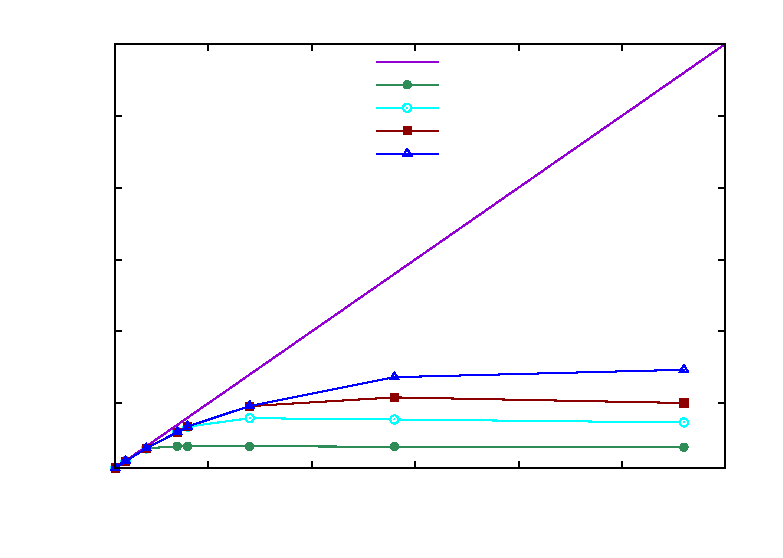
\includegraphics{plot-Tc-s_nogatherInt_00_500_selected_56}}%
    \gplfronttext
  \end{picture}%
\endgroup
}
      \caption{Scalabilita dell implementazione UDN con M=56 al variare del tempo di interarrivo}
      \label{fig:scalability_UDN_size56}
    \end{subfigure}
    ~
    \begin{subfigure}[b]{\textwidth}
      \centering
      \addtocounter{subfigure}{-1}
      \renewcommand\thesubfigure{\alph{subfigure}2}
      \resizebox{\columnwidth}{!}{% GNUPLOT: LaTeX picture with Postscript
\begingroup
  \makeatletter
  \providecommand\color[2][]{%
    \GenericError{(gnuplot) \space\space\space\@spaces}{%
      Package color not loaded in conjunction with
      terminal option `colourtext'%
    }{See the gnuplot documentation for explanation.%
    }{Either use 'blacktext' in gnuplot or load the package
      color.sty in LaTeX.}%
    \renewcommand\color[2][]{}%
  }%
  \providecommand\includegraphics[2][]{%
    \GenericError{(gnuplot) \space\space\space\@spaces}{%
      Package graphicx or graphics not loaded%
    }{See the gnuplot documentation for explanation.%
    }{The gnuplot epslatex terminal needs graphicx.sty or graphics.sty.}%
    \renewcommand\includegraphics[2][]{}%
  }%
  \providecommand\rotatebox[2]{#2}%
  \@ifundefined{ifGPcolor}{%
    \newif\ifGPcolor
    \GPcolortrue
  }{}%
  \@ifundefined{ifGPblacktext}{%
    \newif\ifGPblacktext
    \GPblacktexttrue
  }{}%
  % define a \g@addto@macro without @ in the name:
  \let\gplgaddtomacro\g@addto@macro
  % define empty templates for all commands taking text:
  \gdef\gplbacktext{}%
  \gdef\gplfronttext{}%
  \makeatother
  \ifGPblacktext
    % no textcolor at all
    \def\colorrgb#1{}%
    \def\colorgray#1{}%
  \else
    % gray or color?
    \ifGPcolor
      \def\colorrgb#1{\color[rgb]{#1}}%
      \def\colorgray#1{\color[gray]{#1}}%
      \expandafter\def\csname LTw\endcsname{\color{white}}%
      \expandafter\def\csname LTb\endcsname{\color{black}}%
      \expandafter\def\csname LTa\endcsname{\color{black}}%
      \expandafter\def\csname LT0\endcsname{\color[rgb]{1,0,0}}%
      \expandafter\def\csname LT1\endcsname{\color[rgb]{0,1,0}}%
      \expandafter\def\csname LT2\endcsname{\color[rgb]{0,0,1}}%
      \expandafter\def\csname LT3\endcsname{\color[rgb]{1,0,1}}%
      \expandafter\def\csname LT4\endcsname{\color[rgb]{0,1,1}}%
      \expandafter\def\csname LT5\endcsname{\color[rgb]{1,1,0}}%
      \expandafter\def\csname LT6\endcsname{\color[rgb]{0,0,0}}%
      \expandafter\def\csname LT7\endcsname{\color[rgb]{1,0.3,0}}%
      \expandafter\def\csname LT8\endcsname{\color[rgb]{0.5,0.5,0.5}}%
    \else
      % gray
      \def\colorrgb#1{\color{black}}%
      \def\colorgray#1{\color[gray]{#1}}%
      \expandafter\def\csname LTw\endcsname{\color{white}}%
      \expandafter\def\csname LTb\endcsname{\color{black}}%
      \expandafter\def\csname LTa\endcsname{\color{black}}%
      \expandafter\def\csname LT0\endcsname{\color{black}}%
      \expandafter\def\csname LT1\endcsname{\color{black}}%
      \expandafter\def\csname LT2\endcsname{\color{black}}%
      \expandafter\def\csname LT3\endcsname{\color{black}}%
      \expandafter\def\csname LT4\endcsname{\color{black}}%
      \expandafter\def\csname LT5\endcsname{\color{black}}%
      \expandafter\def\csname LT6\endcsname{\color{black}}%
      \expandafter\def\csname LT7\endcsname{\color{black}}%
      \expandafter\def\csname LT8\endcsname{\color{black}}%
    \fi
  \fi
  \setlength{\unitlength}{0.0500bp}%
  \begin{picture}(7200.00,5040.00)%
    \gplgaddtomacro\gplbacktext{%
      \csname LTb\endcsname%
      \put(814,1325){\makebox(0,0)[r]{\strut{} 10}}%
      \put(814,2015){\makebox(0,0)[r]{\strut{} 20}}%
      \put(814,2705){\makebox(0,0)[r]{\strut{} 30}}%
      \put(814,3395){\makebox(0,0)[r]{\strut{} 40}}%
      \put(814,4085){\makebox(0,0)[r]{\strut{} 50}}%
      \put(814,4775){\makebox(0,0)[r]{\strut{} 60}}%
      \put(1839,484){\makebox(0,0){\strut{} 10}}%
      \put(2832,484){\makebox(0,0){\strut{} 20}}%
      \put(3825,484){\makebox(0,0){\strut{} 30}}%
      \put(4818,484){\makebox(0,0){\strut{} 40}}%
      \put(5810,484){\makebox(0,0){\strut{} 50}}%
      \put(6803,484){\makebox(0,0){\strut{} 60}}%
      \put(176,2739){\rotatebox{-270}{\makebox(0,0){\strut{}scalability}}}%
      \put(3874,154){\makebox(0,0){\strut{}$n$ parallel degree}}%
    }%
    \gplgaddtomacro\gplfronttext{%
      \csname LTb\endcsname%
      \put(3322,4602){\makebox(0,0)[r]{\strut{}ideal scalability}}%
      \csname LTb\endcsname%
      \put(3322,4382){\makebox(0,0)[r]{\strut{}$T_A$ 150000 $\tau$}}%
      \csname LTb\endcsname%
      \put(3322,4162){\makebox(0,0)[r]{\strut{}$T_A$ 80000 $\tau$}}%
      \csname LTb\endcsname%
      \put(3322,3942){\makebox(0,0)[r]{\strut{}$T_A$ 50000 $\tau$}}%
      \csname LTb\endcsname%
      \put(3322,3722){\makebox(0,0)[r]{\strut{}$T_A$ 35000 $\tau$}}%
      \csname LTb\endcsname%
      \put(3322,3502){\makebox(0,0)[r]{\strut{}$T_A$ 20000 $\tau$}}%
    }%
    \gplbacktext
    \put(0,0){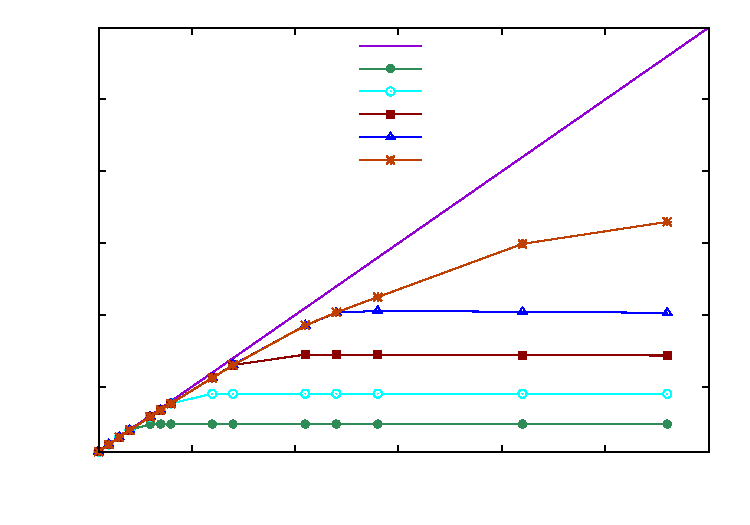
\includegraphics{plot-Tc-s_nogatherInt_00_500_selected_168}}%
    \gplfronttext
  \end{picture}%
\endgroup
}
      \caption{Scalabilita dell implementazione UDN con M=168 al variare del tempo di interarrivo}
      \label{fig:scalability_UDN_size168}
    \end{subfigure}
    ~
    \begin{subfigure}[b]{\textwidth}
      \centering
      \addtocounter{subfigure}{-1}
      \renewcommand\thesubfigure{\alph{subfigure}3}
      \resizebox{\columnwidth}{!}{% GNUPLOT: LaTeX picture with Postscript
\begingroup
  \makeatletter
  \providecommand\color[2][]{%
    \GenericError{(gnuplot) \space\space\space\@spaces}{%
      Package color not loaded in conjunction with
      terminal option `colourtext'%
    }{See the gnuplot documentation for explanation.%
    }{Either use 'blacktext' in gnuplot or load the package
      color.sty in LaTeX.}%
    \renewcommand\color[2][]{}%
  }%
  \providecommand\includegraphics[2][]{%
    \GenericError{(gnuplot) \space\space\space\@spaces}{%
      Package graphicx or graphics not loaded%
    }{See the gnuplot documentation for explanation.%
    }{The gnuplot epslatex terminal needs graphicx.sty or graphics.sty.}%
    \renewcommand\includegraphics[2][]{}%
  }%
  \providecommand\rotatebox[2]{#2}%
  \@ifundefined{ifGPcolor}{%
    \newif\ifGPcolor
    \GPcolortrue
  }{}%
  \@ifundefined{ifGPblacktext}{%
    \newif\ifGPblacktext
    \GPblacktexttrue
  }{}%
  % define a \g@addto@macro without @ in the name:
  \let\gplgaddtomacro\g@addto@macro
  % define empty templates for all commands taking text:
  \gdef\gplbacktext{}%
  \gdef\gplfronttext{}%
  \makeatother
  \ifGPblacktext
    % no textcolor at all
    \def\colorrgb#1{}%
    \def\colorgray#1{}%
  \else
    % gray or color?
    \ifGPcolor
      \def\colorrgb#1{\color[rgb]{#1}}%
      \def\colorgray#1{\color[gray]{#1}}%
      \expandafter\def\csname LTw\endcsname{\color{white}}%
      \expandafter\def\csname LTb\endcsname{\color{black}}%
      \expandafter\def\csname LTa\endcsname{\color{black}}%
      \expandafter\def\csname LT0\endcsname{\color[rgb]{1,0,0}}%
      \expandafter\def\csname LT1\endcsname{\color[rgb]{0,1,0}}%
      \expandafter\def\csname LT2\endcsname{\color[rgb]{0,0,1}}%
      \expandafter\def\csname LT3\endcsname{\color[rgb]{1,0,1}}%
      \expandafter\def\csname LT4\endcsname{\color[rgb]{0,1,1}}%
      \expandafter\def\csname LT5\endcsname{\color[rgb]{1,1,0}}%
      \expandafter\def\csname LT6\endcsname{\color[rgb]{0,0,0}}%
      \expandafter\def\csname LT7\endcsname{\color[rgb]{1,0.3,0}}%
      \expandafter\def\csname LT8\endcsname{\color[rgb]{0.5,0.5,0.5}}%
    \else
      % gray
      \def\colorrgb#1{\color{black}}%
      \def\colorgray#1{\color[gray]{#1}}%
      \expandafter\def\csname LTw\endcsname{\color{white}}%
      \expandafter\def\csname LTb\endcsname{\color{black}}%
      \expandafter\def\csname LTa\endcsname{\color{black}}%
      \expandafter\def\csname LT0\endcsname{\color{black}}%
      \expandafter\def\csname LT1\endcsname{\color{black}}%
      \expandafter\def\csname LT2\endcsname{\color{black}}%
      \expandafter\def\csname LT3\endcsname{\color{black}}%
      \expandafter\def\csname LT4\endcsname{\color{black}}%
      \expandafter\def\csname LT5\endcsname{\color{black}}%
      \expandafter\def\csname LT6\endcsname{\color{black}}%
      \expandafter\def\csname LT7\endcsname{\color{black}}%
      \expandafter\def\csname LT8\endcsname{\color{black}}%
    \fi
  \fi
  \setlength{\unitlength}{0.0500bp}%
  \begin{picture}(7200.00,5040.00)%
    \gplgaddtomacro\gplbacktext{%
      \csname LTb\endcsname%
      \put(814,1325){\makebox(0,0)[r]{\strut{} 10}}%
      \put(814,2015){\makebox(0,0)[r]{\strut{} 20}}%
      \put(814,2705){\makebox(0,0)[r]{\strut{} 30}}%
      \put(814,3395){\makebox(0,0)[r]{\strut{} 40}}%
      \put(814,4085){\makebox(0,0)[r]{\strut{} 50}}%
      \put(814,4775){\makebox(0,0)[r]{\strut{} 60}}%
      \put(1839,484){\makebox(0,0){\strut{} 10}}%
      \put(2832,484){\makebox(0,0){\strut{} 20}}%
      \put(3825,484){\makebox(0,0){\strut{} 30}}%
      \put(4818,484){\makebox(0,0){\strut{} 40}}%
      \put(5810,484){\makebox(0,0){\strut{} 50}}%
      \put(6803,484){\makebox(0,0){\strut{} 60}}%
      \put(176,2739){\rotatebox{-270}{\makebox(0,0){\strut{}scalability}}}%
      \put(3874,154){\makebox(0,0){\strut{}$n$ parallel degree}}%
    }%
    \gplgaddtomacro\gplfronttext{%
      \csname LTb\endcsname%
      \put(3322,4602){\makebox(0,0)[r]{\strut{}ideal scalability}}%
      \csname LTb\endcsname%
      \put(3322,4382){\makebox(0,0)[r]{\strut{}$T_A$ 250000 $\tau$}}%
      \csname LTb\endcsname%
      \put(3322,4162){\makebox(0,0)[r]{\strut{}$T_A$ 150000 $\tau$}}%
      \csname LTb\endcsname%
      \put(3322,3942){\makebox(0,0)[r]{\strut{}$T_A$ 100000 $\tau$}}%
      \csname LTb\endcsname%
      \put(3322,3722){\makebox(0,0)[r]{\strut{}$T_A$ 80000 $\tau$}}%
      \csname LTb\endcsname%
      \put(3322,3502){\makebox(0,0)[r]{\strut{}$T_A$ 50000 $\tau$}}%
    }%
    \gplbacktext
    \put(0,0){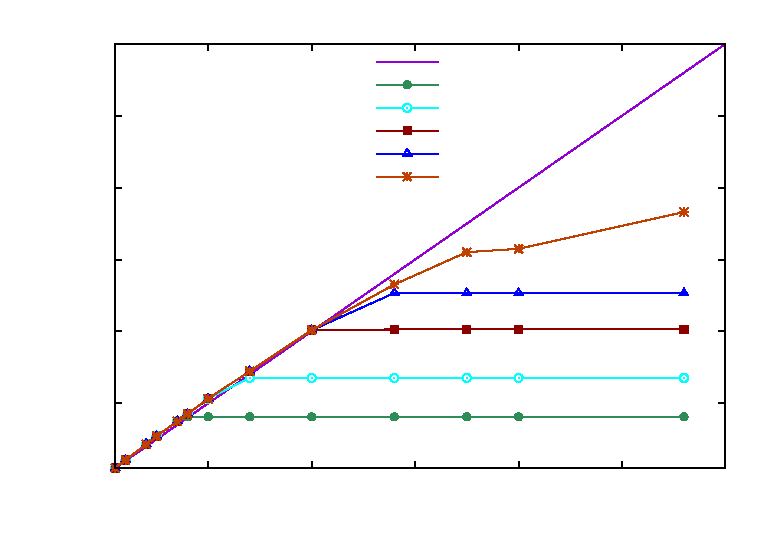
\includegraphics{plot-Tc-s_nogatherInt_00_500_selected_280}}%
    \gplfronttext
  \end{picture}%
\endgroup
}
      \caption{Scalabilita dell implementazione UDN con M=280 al variare del tempo di interarrivo}
      \label{fig:scalability_UDN_size280}
    \end{subfigure}
    \label{fig:allScalbility_UDN}
  \end{subfigure}
  \hspace{2ex}
  \begin{subfigure}[b]{.5\columnwidth}
    \centering
    \renewcommand\thesubfigure{\alph{subfigure}}
    \caption{Implementazione con solo SM}
    \begin{subfigure}[b]{\textwidth}
      \centering
      \addtocounter{subfigure}{-1}
      \renewcommand\thesubfigure{\alph{subfigure}1}
      \resizebox{\columnwidth}{!}{% GNUPLOT: LaTeX picture with Postscript
\begingroup
  \makeatletter
  \providecommand\color[2][]{%
    \GenericError{(gnuplot) \space\space\space\@spaces}{%
      Package color not loaded in conjunction with
      terminal option `colourtext'%
    }{See the gnuplot documentation for explanation.%
    }{Either use 'blacktext' in gnuplot or load the package
      color.sty in LaTeX.}%
    \renewcommand\color[2][]{}%
  }%
  \providecommand\includegraphics[2][]{%
    \GenericError{(gnuplot) \space\space\space\@spaces}{%
      Package graphicx or graphics not loaded%
    }{See the gnuplot documentation for explanation.%
    }{The gnuplot epslatex terminal needs graphicx.sty or graphics.sty.}%
    \renewcommand\includegraphics[2][]{}%
  }%
  \providecommand\rotatebox[2]{#2}%
  \@ifundefined{ifGPcolor}{%
    \newif\ifGPcolor
    \GPcolortrue
  }{}%
  \@ifundefined{ifGPblacktext}{%
    \newif\ifGPblacktext
    \GPblacktexttrue
  }{}%
  % define a \g@addto@macro without @ in the name:
  \let\gplgaddtomacro\g@addto@macro
  % define empty templates for all commands taking text:
  \gdef\gplbacktext{}%
  \gdef\gplfronttext{}%
  \makeatother
  \ifGPblacktext
    % no textcolor at all
    \def\colorrgb#1{}%
    \def\colorgray#1{}%
  \else
    % gray or color?
    \ifGPcolor
      \def\colorrgb#1{\color[rgb]{#1}}%
      \def\colorgray#1{\color[gray]{#1}}%
      \expandafter\def\csname LTw\endcsname{\color{white}}%
      \expandafter\def\csname LTb\endcsname{\color{black}}%
      \expandafter\def\csname LTa\endcsname{\color{black}}%
      \expandafter\def\csname LT0\endcsname{\color[rgb]{1,0,0}}%
      \expandafter\def\csname LT1\endcsname{\color[rgb]{0,1,0}}%
      \expandafter\def\csname LT2\endcsname{\color[rgb]{0,0,1}}%
      \expandafter\def\csname LT3\endcsname{\color[rgb]{1,0,1}}%
      \expandafter\def\csname LT4\endcsname{\color[rgb]{0,1,1}}%
      \expandafter\def\csname LT5\endcsname{\color[rgb]{1,1,0}}%
      \expandafter\def\csname LT6\endcsname{\color[rgb]{0,0,0}}%
      \expandafter\def\csname LT7\endcsname{\color[rgb]{1,0.3,0}}%
      \expandafter\def\csname LT8\endcsname{\color[rgb]{0.5,0.5,0.5}}%
    \else
      % gray
      \def\colorrgb#1{\color{black}}%
      \def\colorgray#1{\color[gray]{#1}}%
      \expandafter\def\csname LTw\endcsname{\color{white}}%
      \expandafter\def\csname LTb\endcsname{\color{black}}%
      \expandafter\def\csname LTa\endcsname{\color{black}}%
      \expandafter\def\csname LT0\endcsname{\color{black}}%
      \expandafter\def\csname LT1\endcsname{\color{black}}%
      \expandafter\def\csname LT2\endcsname{\color{black}}%
      \expandafter\def\csname LT3\endcsname{\color{black}}%
      \expandafter\def\csname LT4\endcsname{\color{black}}%
      \expandafter\def\csname LT5\endcsname{\color{black}}%
      \expandafter\def\csname LT6\endcsname{\color{black}}%
      \expandafter\def\csname LT7\endcsname{\color{black}}%
      \expandafter\def\csname LT8\endcsname{\color{black}}%
    \fi
  \fi
  \setlength{\unitlength}{0.0500bp}%
  \begin{picture}(7200.00,5040.00)%
    \gplgaddtomacro\gplbacktext{%
      \csname LTb\endcsname%
      \put(814,1325){\makebox(0,0)[r]{\strut{} 10}}%
      \put(814,2015){\makebox(0,0)[r]{\strut{} 20}}%
      \put(814,2705){\makebox(0,0)[r]{\strut{} 30}}%
      \put(814,3395){\makebox(0,0)[r]{\strut{} 40}}%
      \put(814,4085){\makebox(0,0)[r]{\strut{} 50}}%
      \put(814,4775){\makebox(0,0)[r]{\strut{} 60}}%
      \put(1839,484){\makebox(0,0){\strut{} 10}}%
      \put(2832,484){\makebox(0,0){\strut{} 20}}%
      \put(3825,484){\makebox(0,0){\strut{} 30}}%
      \put(4818,484){\makebox(0,0){\strut{} 40}}%
      \put(5810,484){\makebox(0,0){\strut{} 50}}%
      \put(6803,484){\makebox(0,0){\strut{} 60}}%
      \put(176,2739){\rotatebox{-270}{\makebox(0,0){\strut{}scalability}}}%
      \put(3874,154){\makebox(0,0){\strut{}$n$ parallel degree}}%
    }%
    \gplgaddtomacro\gplfronttext{%
      \csname LTb\endcsname%
      \put(3322,4602){\makebox(0,0)[r]{\strut{}ideal scalability}}%
      \csname LTb\endcsname%
      \put(3322,4382){\makebox(0,0)[r]{\strut{}$T_A$ 20000 $\tau$}}%
      \csname LTb\endcsname%
      \put(3322,4162){\makebox(0,0)[r]{\strut{}$T_A$ 10000 $\tau$}}%
      \csname LTb\endcsname%
      \put(3322,3942){\makebox(0,0)[r]{\strut{}$T_A$ 7000 $\tau$}}%
      \csname LTb\endcsname%
      \put(3322,3722){\makebox(0,0)[r]{\strut{}$T_A$ 4000 $\tau$}}%
    }%
    \gplbacktext
    \put(0,0){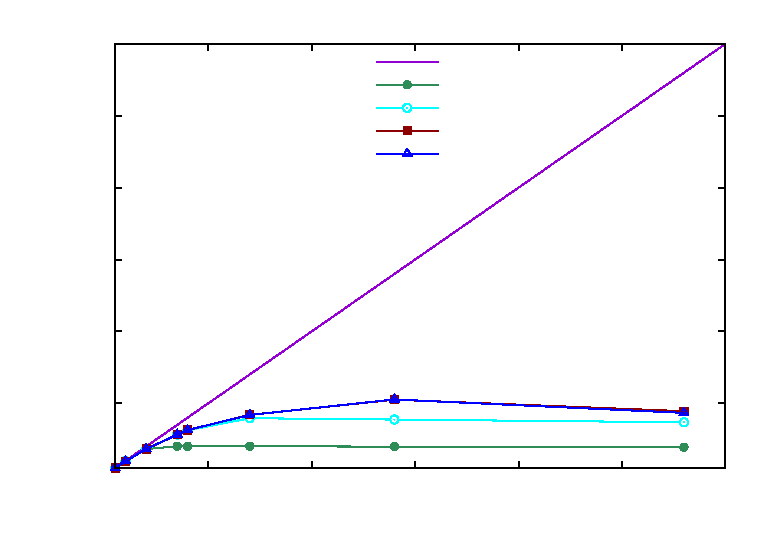
\includegraphics{plot-Tc-s_nogatherInt_11_500_selected_56}}%
    \gplfronttext
  \end{picture}%
\endgroup
}
      \caption{Scalabilita dell implementazione SM con M=56 al variare del tempo di interarrivo}
      \label{fig:scalability_SM_size56}
    \end{subfigure}
    ~
    \begin{subfigure}[b]{\textwidth}
      \centering
      \addtocounter{subfigure}{-1}
      \renewcommand\thesubfigure{\alph{subfigure}2}
      \resizebox{\columnwidth}{!}{% GNUPLOT: LaTeX picture with Postscript
\begingroup
  \makeatletter
  \providecommand\color[2][]{%
    \GenericError{(gnuplot) \space\space\space\@spaces}{%
      Package color not loaded in conjunction with
      terminal option `colourtext'%
    }{See the gnuplot documentation for explanation.%
    }{Either use 'blacktext' in gnuplot or load the package
      color.sty in LaTeX.}%
    \renewcommand\color[2][]{}%
  }%
  \providecommand\includegraphics[2][]{%
    \GenericError{(gnuplot) \space\space\space\@spaces}{%
      Package graphicx or graphics not loaded%
    }{See the gnuplot documentation for explanation.%
    }{The gnuplot epslatex terminal needs graphicx.sty or graphics.sty.}%
    \renewcommand\includegraphics[2][]{}%
  }%
  \providecommand\rotatebox[2]{#2}%
  \@ifundefined{ifGPcolor}{%
    \newif\ifGPcolor
    \GPcolortrue
  }{}%
  \@ifundefined{ifGPblacktext}{%
    \newif\ifGPblacktext
    \GPblacktexttrue
  }{}%
  % define a \g@addto@macro without @ in the name:
  \let\gplgaddtomacro\g@addto@macro
  % define empty templates for all commands taking text:
  \gdef\gplbacktext{}%
  \gdef\gplfronttext{}%
  \makeatother
  \ifGPblacktext
    % no textcolor at all
    \def\colorrgb#1{}%
    \def\colorgray#1{}%
  \else
    % gray or color?
    \ifGPcolor
      \def\colorrgb#1{\color[rgb]{#1}}%
      \def\colorgray#1{\color[gray]{#1}}%
      \expandafter\def\csname LTw\endcsname{\color{white}}%
      \expandafter\def\csname LTb\endcsname{\color{black}}%
      \expandafter\def\csname LTa\endcsname{\color{black}}%
      \expandafter\def\csname LT0\endcsname{\color[rgb]{1,0,0}}%
      \expandafter\def\csname LT1\endcsname{\color[rgb]{0,1,0}}%
      \expandafter\def\csname LT2\endcsname{\color[rgb]{0,0,1}}%
      \expandafter\def\csname LT3\endcsname{\color[rgb]{1,0,1}}%
      \expandafter\def\csname LT4\endcsname{\color[rgb]{0,1,1}}%
      \expandafter\def\csname LT5\endcsname{\color[rgb]{1,1,0}}%
      \expandafter\def\csname LT6\endcsname{\color[rgb]{0,0,0}}%
      \expandafter\def\csname LT7\endcsname{\color[rgb]{1,0.3,0}}%
      \expandafter\def\csname LT8\endcsname{\color[rgb]{0.5,0.5,0.5}}%
    \else
      % gray
      \def\colorrgb#1{\color{black}}%
      \def\colorgray#1{\color[gray]{#1}}%
      \expandafter\def\csname LTw\endcsname{\color{white}}%
      \expandafter\def\csname LTb\endcsname{\color{black}}%
      \expandafter\def\csname LTa\endcsname{\color{black}}%
      \expandafter\def\csname LT0\endcsname{\color{black}}%
      \expandafter\def\csname LT1\endcsname{\color{black}}%
      \expandafter\def\csname LT2\endcsname{\color{black}}%
      \expandafter\def\csname LT3\endcsname{\color{black}}%
      \expandafter\def\csname LT4\endcsname{\color{black}}%
      \expandafter\def\csname LT5\endcsname{\color{black}}%
      \expandafter\def\csname LT6\endcsname{\color{black}}%
      \expandafter\def\csname LT7\endcsname{\color{black}}%
      \expandafter\def\csname LT8\endcsname{\color{black}}%
    \fi
  \fi
  \setlength{\unitlength}{0.0500bp}%
  \begin{picture}(7200.00,5040.00)%
    \gplgaddtomacro\gplbacktext{%
      \csname LTb\endcsname%
      \put(814,1325){\makebox(0,0)[r]{\strut{} 10}}%
      \put(814,2015){\makebox(0,0)[r]{\strut{} 20}}%
      \put(814,2705){\makebox(0,0)[r]{\strut{} 30}}%
      \put(814,3395){\makebox(0,0)[r]{\strut{} 40}}%
      \put(814,4085){\makebox(0,0)[r]{\strut{} 50}}%
      \put(814,4775){\makebox(0,0)[r]{\strut{} 60}}%
      \put(1839,484){\makebox(0,0){\strut{} 10}}%
      \put(2832,484){\makebox(0,0){\strut{} 20}}%
      \put(3825,484){\makebox(0,0){\strut{} 30}}%
      \put(4818,484){\makebox(0,0){\strut{} 40}}%
      \put(5810,484){\makebox(0,0){\strut{} 50}}%
      \put(6803,484){\makebox(0,0){\strut{} 60}}%
      \put(176,2739){\rotatebox{-270}{\makebox(0,0){\strut{}scalability}}}%
      \put(3874,154){\makebox(0,0){\strut{}$n$ parallel degree}}%
    }%
    \gplgaddtomacro\gplfronttext{%
      \csname LTb\endcsname%
      \put(3322,4602){\makebox(0,0)[r]{\strut{}ideal scalability}}%
      \csname LTb\endcsname%
      \put(3322,4382){\makebox(0,0)[r]{\strut{}$T_A$ 150000 $\tau$}}%
      \csname LTb\endcsname%
      \put(3322,4162){\makebox(0,0)[r]{\strut{}$T_A$ 80000 $\tau$}}%
      \csname LTb\endcsname%
      \put(3322,3942){\makebox(0,0)[r]{\strut{}$T_A$ 50000 $\tau$}}%
      \csname LTb\endcsname%
      \put(3322,3722){\makebox(0,0)[r]{\strut{}$T_A$ 35000 $\tau$}}%
      \csname LTb\endcsname%
      \put(3322,3502){\makebox(0,0)[r]{\strut{}$T_A$ 20000 $\tau$}}%
    }%
    \gplbacktext
    \put(0,0){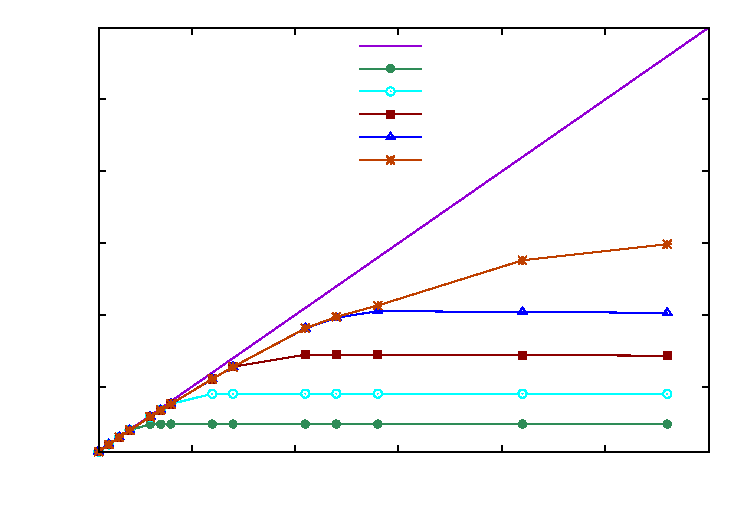
\includegraphics{plot-Tc-s_nogatherInt_11_500_selected_168}}%
    \gplfronttext
  \end{picture}%
\endgroup
}
      \caption{Scalabilita dell implementazione SM con M=168 al variare del tempo di interarrivo}
      \label{fig:scalability_SM_size168}
    \end{subfigure}
    ~
    \begin{subfigure}[b]{\textwidth}
      \centering
      \addtocounter{subfigure}{-1}
      \renewcommand\thesubfigure{\alph{subfigure}3}
      \resizebox{\columnwidth}{!}{% GNUPLOT: LaTeX picture with Postscript
\begingroup
  \makeatletter
  \providecommand\color[2][]{%
    \GenericError{(gnuplot) \space\space\space\@spaces}{%
      Package color not loaded in conjunction with
      terminal option `colourtext'%
    }{See the gnuplot documentation for explanation.%
    }{Either use 'blacktext' in gnuplot or load the package
      color.sty in LaTeX.}%
    \renewcommand\color[2][]{}%
  }%
  \providecommand\includegraphics[2][]{%
    \GenericError{(gnuplot) \space\space\space\@spaces}{%
      Package graphicx or graphics not loaded%
    }{See the gnuplot documentation for explanation.%
    }{The gnuplot epslatex terminal needs graphicx.sty or graphics.sty.}%
    \renewcommand\includegraphics[2][]{}%
  }%
  \providecommand\rotatebox[2]{#2}%
  \@ifundefined{ifGPcolor}{%
    \newif\ifGPcolor
    \GPcolortrue
  }{}%
  \@ifundefined{ifGPblacktext}{%
    \newif\ifGPblacktext
    \GPblacktexttrue
  }{}%
  % define a \g@addto@macro without @ in the name:
  \let\gplgaddtomacro\g@addto@macro
  % define empty templates for all commands taking text:
  \gdef\gplbacktext{}%
  \gdef\gplfronttext{}%
  \makeatother
  \ifGPblacktext
    % no textcolor at all
    \def\colorrgb#1{}%
    \def\colorgray#1{}%
  \else
    % gray or color?
    \ifGPcolor
      \def\colorrgb#1{\color[rgb]{#1}}%
      \def\colorgray#1{\color[gray]{#1}}%
      \expandafter\def\csname LTw\endcsname{\color{white}}%
      \expandafter\def\csname LTb\endcsname{\color{black}}%
      \expandafter\def\csname LTa\endcsname{\color{black}}%
      \expandafter\def\csname LT0\endcsname{\color[rgb]{1,0,0}}%
      \expandafter\def\csname LT1\endcsname{\color[rgb]{0,1,0}}%
      \expandafter\def\csname LT2\endcsname{\color[rgb]{0,0,1}}%
      \expandafter\def\csname LT3\endcsname{\color[rgb]{1,0,1}}%
      \expandafter\def\csname LT4\endcsname{\color[rgb]{0,1,1}}%
      \expandafter\def\csname LT5\endcsname{\color[rgb]{1,1,0}}%
      \expandafter\def\csname LT6\endcsname{\color[rgb]{0,0,0}}%
      \expandafter\def\csname LT7\endcsname{\color[rgb]{1,0.3,0}}%
      \expandafter\def\csname LT8\endcsname{\color[rgb]{0.5,0.5,0.5}}%
    \else
      % gray
      \def\colorrgb#1{\color{black}}%
      \def\colorgray#1{\color[gray]{#1}}%
      \expandafter\def\csname LTw\endcsname{\color{white}}%
      \expandafter\def\csname LTb\endcsname{\color{black}}%
      \expandafter\def\csname LTa\endcsname{\color{black}}%
      \expandafter\def\csname LT0\endcsname{\color{black}}%
      \expandafter\def\csname LT1\endcsname{\color{black}}%
      \expandafter\def\csname LT2\endcsname{\color{black}}%
      \expandafter\def\csname LT3\endcsname{\color{black}}%
      \expandafter\def\csname LT4\endcsname{\color{black}}%
      \expandafter\def\csname LT5\endcsname{\color{black}}%
      \expandafter\def\csname LT6\endcsname{\color{black}}%
      \expandafter\def\csname LT7\endcsname{\color{black}}%
      \expandafter\def\csname LT8\endcsname{\color{black}}%
    \fi
  \fi
  \setlength{\unitlength}{0.0500bp}%
  \begin{picture}(7200.00,5040.00)%
    \gplgaddtomacro\gplbacktext{%
      \csname LTb\endcsname%
      \put(814,1325){\makebox(0,0)[r]{\strut{} 10}}%
      \put(814,2015){\makebox(0,0)[r]{\strut{} 20}}%
      \put(814,2705){\makebox(0,0)[r]{\strut{} 30}}%
      \put(814,3395){\makebox(0,0)[r]{\strut{} 40}}%
      \put(814,4085){\makebox(0,0)[r]{\strut{} 50}}%
      \put(814,4775){\makebox(0,0)[r]{\strut{} 60}}%
      \put(1839,484){\makebox(0,0){\strut{} 10}}%
      \put(2832,484){\makebox(0,0){\strut{} 20}}%
      \put(3825,484){\makebox(0,0){\strut{} 30}}%
      \put(4818,484){\makebox(0,0){\strut{} 40}}%
      \put(5810,484){\makebox(0,0){\strut{} 50}}%
      \put(6803,484){\makebox(0,0){\strut{} 60}}%
      \put(176,2739){\rotatebox{-270}{\makebox(0,0){\strut{}scalability}}}%
      \put(3874,154){\makebox(0,0){\strut{}$n$ parallel degree}}%
    }%
    \gplgaddtomacro\gplfronttext{%
      \csname LTb\endcsname%
      \put(3322,4602){\makebox(0,0)[r]{\strut{}ideal scalability}}%
      \csname LTb\endcsname%
      \put(3322,4382){\makebox(0,0)[r]{\strut{}$T_A$ 250000 $\tau$}}%
      \csname LTb\endcsname%
      \put(3322,4162){\makebox(0,0)[r]{\strut{}$T_A$ 150000 $\tau$}}%
      \csname LTb\endcsname%
      \put(3322,3942){\makebox(0,0)[r]{\strut{}$T_A$ 100000 $\tau$}}%
      \csname LTb\endcsname%
      \put(3322,3722){\makebox(0,0)[r]{\strut{}$T_A$ 80000 $\tau$}}%
      \csname LTb\endcsname%
      \put(3322,3502){\makebox(0,0)[r]{\strut{}$T_A$ 50000 $\tau$}}%
    }%
    \gplbacktext
    \put(0,0){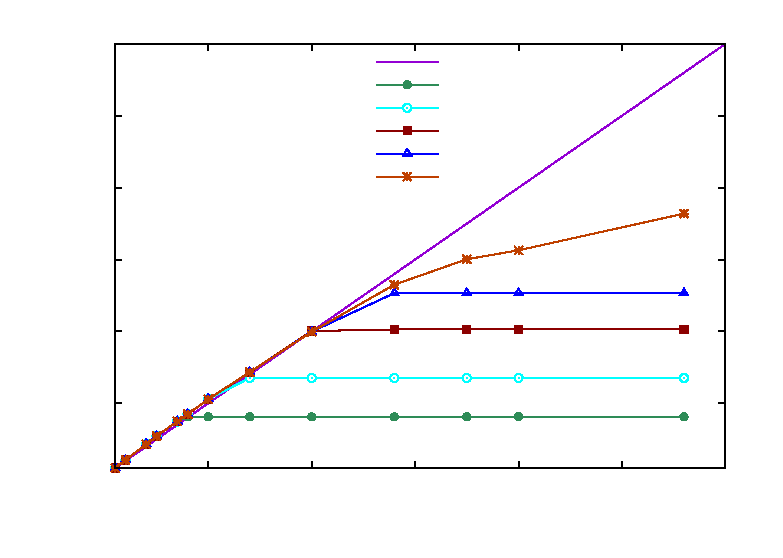
\includegraphics{plot-Tc-s_nogatherInt_11_500_selected_280}}%
    \gplfronttext
  \end{picture}%
\endgroup
}
      \caption{Scalabilita dell implementazione SM con M=280 al variare del tempo di interarrivo}
      \label{fig:scalability_SM_size280}
    \end{subfigure}
    \label{fig:allscalability_SM}
  \end{subfigure}
\end{figure}


%%%%%%%%%%%%%%%%%%%%%%%%%%%%%%%%%%%%%%%%%%%%%%%%%%%%%%%%%%%%%%%%%%%%%%%%%%%%%%%%


\FloatBarrier

\begin{figure}[p]
  \caption{Grafici del tempo di completamento al variare del tempo di interarrivo}
  \begin{subfigure}[b]{.5\columnwidth}
    \centering
    \renewcommand\thesubfigure{\alph{subfigure}}
    %% se vuoi spostare questa caption in fondo devi modificare anche i contatori!
    \caption{Implementazione con solo UDN}
    \begin{subfigure}[b]{\textwidth}
      \centering
      \addtocounter{subfigure}{-1}
      \renewcommand\thesubfigure{\alph{subfigure}1}
      \resizebox{\columnwidth}{!}{% GNUPLOT: LaTeX picture with Postscript
\begingroup
  \makeatletter
  \providecommand\color[2][]{%
    \GenericError{(gnuplot) \space\space\space\@spaces}{%
      Package color not loaded in conjunction with
      terminal option `colourtext'%
    }{See the gnuplot documentation for explanation.%
    }{Either use 'blacktext' in gnuplot or load the package
      color.sty in LaTeX.}%
    \renewcommand\color[2][]{}%
  }%
  \providecommand\includegraphics[2][]{%
    \GenericError{(gnuplot) \space\space\space\@spaces}{%
      Package graphicx or graphics not loaded%
    }{See the gnuplot documentation for explanation.%
    }{The gnuplot epslatex terminal needs graphicx.sty or graphics.sty.}%
    \renewcommand\includegraphics[2][]{}%
  }%
  \providecommand\rotatebox[2]{#2}%
  \@ifundefined{ifGPcolor}{%
    \newif\ifGPcolor
    \GPcolortrue
  }{}%
  \@ifundefined{ifGPblacktext}{%
    \newif\ifGPblacktext
    \GPblacktexttrue
  }{}%
  % define a \g@addto@macro without @ in the name:
  \let\gplgaddtomacro\g@addto@macro
  % define empty templates for all commands taking text:
  \gdef\gplbacktext{}%
  \gdef\gplfronttext{}%
  \makeatother
  \ifGPblacktext
    % no textcolor at all
    \def\colorrgb#1{}%
    \def\colorgray#1{}%
  \else
    % gray or color?
    \ifGPcolor
      \def\colorrgb#1{\color[rgb]{#1}}%
      \def\colorgray#1{\color[gray]{#1}}%
      \expandafter\def\csname LTw\endcsname{\color{white}}%
      \expandafter\def\csname LTb\endcsname{\color{black}}%
      \expandafter\def\csname LTa\endcsname{\color{black}}%
      \expandafter\def\csname LT0\endcsname{\color[rgb]{1,0,0}}%
      \expandafter\def\csname LT1\endcsname{\color[rgb]{0,1,0}}%
      \expandafter\def\csname LT2\endcsname{\color[rgb]{0,0,1}}%
      \expandafter\def\csname LT3\endcsname{\color[rgb]{1,0,1}}%
      \expandafter\def\csname LT4\endcsname{\color[rgb]{0,1,1}}%
      \expandafter\def\csname LT5\endcsname{\color[rgb]{1,1,0}}%
      \expandafter\def\csname LT6\endcsname{\color[rgb]{0,0,0}}%
      \expandafter\def\csname LT7\endcsname{\color[rgb]{1,0.3,0}}%
      \expandafter\def\csname LT8\endcsname{\color[rgb]{0.5,0.5,0.5}}%
    \else
      % gray
      \def\colorrgb#1{\color{black}}%
      \def\colorgray#1{\color[gray]{#1}}%
      \expandafter\def\csname LTw\endcsname{\color{white}}%
      \expandafter\def\csname LTb\endcsname{\color{black}}%
      \expandafter\def\csname LTa\endcsname{\color{black}}%
      \expandafter\def\csname LT0\endcsname{\color{black}}%
      \expandafter\def\csname LT1\endcsname{\color{black}}%
      \expandafter\def\csname LT2\endcsname{\color{black}}%
      \expandafter\def\csname LT3\endcsname{\color{black}}%
      \expandafter\def\csname LT4\endcsname{\color{black}}%
      \expandafter\def\csname LT5\endcsname{\color{black}}%
      \expandafter\def\csname LT6\endcsname{\color{black}}%
      \expandafter\def\csname LT7\endcsname{\color{black}}%
      \expandafter\def\csname LT8\endcsname{\color{black}}%
    \fi
  \fi
  \setlength{\unitlength}{0.0500bp}%
  \begin{picture}(7200.00,5040.00)%
    \gplgaddtomacro\gplbacktext{%
      \csname LTb\endcsname%
      \put(946,704){\makebox(0,0)[r]{\strut{} 1}}%
      \put(946,2740){\makebox(0,0)[r]{\strut{} 10}}%
      \put(946,4775){\makebox(0,0)[r]{\strut{} 100}}%
      \put(1951,484){\makebox(0,0){\strut{} 10}}%
      \put(2922,484){\makebox(0,0){\strut{} 20}}%
      \put(3892,484){\makebox(0,0){\strut{} 30}}%
      \put(4862,484){\makebox(0,0){\strut{} 40}}%
      \put(5833,484){\makebox(0,0){\strut{} 50}}%
      \put(6803,484){\makebox(0,0){\strut{} 60}}%
      \put(176,2739){\rotatebox{-270}{\makebox(0,0){\strut{}$T_{\textrm{C}}$ complete time (ms)}}}%
      \put(3940,154){\makebox(0,0){\strut{}parallel degree}}%
    }%
    \gplgaddtomacro\gplfronttext{%
      \csname LTb\endcsname%
      \put(3190,4602){\makebox(0,0)[r]{\strut{}$T_A$ 23.133 $\mu\mathrm{sec}$}}%
      \csname LTb\endcsname%
      \put(3190,4382){\makebox(0,0)[r]{\strut{}$T_A$ 11.566 $\mu\mathrm{sec}$}}%
      \csname LTb\endcsname%
      \put(3190,4162){\makebox(0,0)[r]{\strut{}$T_A$ 8.096 $\mu\mathrm{sec}$}}%
      \csname LTb\endcsname%
      \put(3190,3942){\makebox(0,0)[r]{\strut{}$T_A$ 4.627 $\mu\mathrm{sec}$}}%
    }%
    \gplbacktext
    \put(0,0){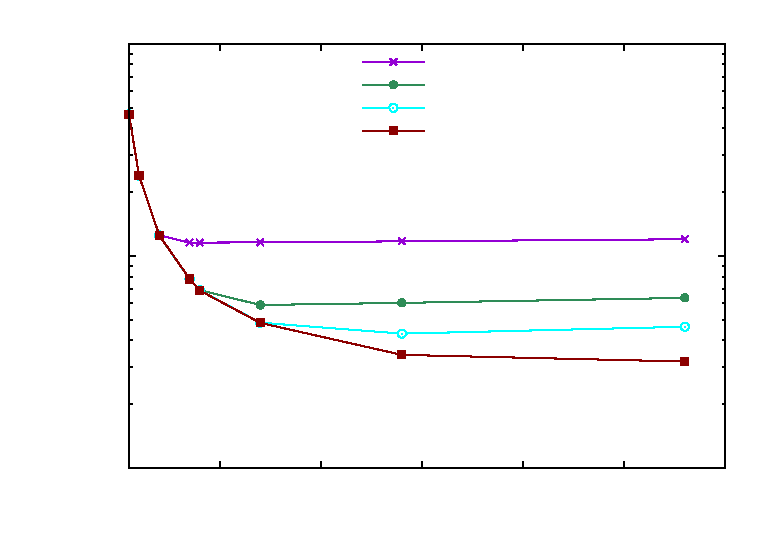
\includegraphics{plot-Tc_nogatherInt_00_500_selected_56}}%
    \gplfronttext
  \end{picture}%
\endgroup
}
      \caption{Tempo di completamento dell implementazione UDN con M=56 al variare del tempo di interarrivo}
      \label{fig:scalability_UDN_size56}
    \end{subfigure}
    ~
    \begin{subfigure}[b]{\textwidth}
      \centering
      \addtocounter{subfigure}{-1}
      \renewcommand\thesubfigure{\alph{subfigure}2}
      \resizebox{\columnwidth}{!}{% GNUPLOT: LaTeX picture with Postscript
\begingroup
  \makeatletter
  \providecommand\color[2][]{%
    \GenericError{(gnuplot) \space\space\space\@spaces}{%
      Package color not loaded in conjunction with
      terminal option `colourtext'%
    }{See the gnuplot documentation for explanation.%
    }{Either use 'blacktext' in gnuplot or load the package
      color.sty in LaTeX.}%
    \renewcommand\color[2][]{}%
  }%
  \providecommand\includegraphics[2][]{%
    \GenericError{(gnuplot) \space\space\space\@spaces}{%
      Package graphicx or graphics not loaded%
    }{See the gnuplot documentation for explanation.%
    }{The gnuplot epslatex terminal needs graphicx.sty or graphics.sty.}%
    \renewcommand\includegraphics[2][]{}%
  }%
  \providecommand\rotatebox[2]{#2}%
  \@ifundefined{ifGPcolor}{%
    \newif\ifGPcolor
    \GPcolortrue
  }{}%
  \@ifundefined{ifGPblacktext}{%
    \newif\ifGPblacktext
    \GPblacktexttrue
  }{}%
  % define a \g@addto@macro without @ in the name:
  \let\gplgaddtomacro\g@addto@macro
  % define empty templates for all commands taking text:
  \gdef\gplbacktext{}%
  \gdef\gplfronttext{}%
  \makeatother
  \ifGPblacktext
    % no textcolor at all
    \def\colorrgb#1{}%
    \def\colorgray#1{}%
  \else
    % gray or color?
    \ifGPcolor
      \def\colorrgb#1{\color[rgb]{#1}}%
      \def\colorgray#1{\color[gray]{#1}}%
      \expandafter\def\csname LTw\endcsname{\color{white}}%
      \expandafter\def\csname LTb\endcsname{\color{black}}%
      \expandafter\def\csname LTa\endcsname{\color{black}}%
      \expandafter\def\csname LT0\endcsname{\color[rgb]{1,0,0}}%
      \expandafter\def\csname LT1\endcsname{\color[rgb]{0,1,0}}%
      \expandafter\def\csname LT2\endcsname{\color[rgb]{0,0,1}}%
      \expandafter\def\csname LT3\endcsname{\color[rgb]{1,0,1}}%
      \expandafter\def\csname LT4\endcsname{\color[rgb]{0,1,1}}%
      \expandafter\def\csname LT5\endcsname{\color[rgb]{1,1,0}}%
      \expandafter\def\csname LT6\endcsname{\color[rgb]{0,0,0}}%
      \expandafter\def\csname LT7\endcsname{\color[rgb]{1,0.3,0}}%
      \expandafter\def\csname LT8\endcsname{\color[rgb]{0.5,0.5,0.5}}%
    \else
      % gray
      \def\colorrgb#1{\color{black}}%
      \def\colorgray#1{\color[gray]{#1}}%
      \expandafter\def\csname LTw\endcsname{\color{white}}%
      \expandafter\def\csname LTb\endcsname{\color{black}}%
      \expandafter\def\csname LTa\endcsname{\color{black}}%
      \expandafter\def\csname LT0\endcsname{\color{black}}%
      \expandafter\def\csname LT1\endcsname{\color{black}}%
      \expandafter\def\csname LT2\endcsname{\color{black}}%
      \expandafter\def\csname LT3\endcsname{\color{black}}%
      \expandafter\def\csname LT4\endcsname{\color{black}}%
      \expandafter\def\csname LT5\endcsname{\color{black}}%
      \expandafter\def\csname LT6\endcsname{\color{black}}%
      \expandafter\def\csname LT7\endcsname{\color{black}}%
      \expandafter\def\csname LT8\endcsname{\color{black}}%
    \fi
  \fi
  \setlength{\unitlength}{0.0500bp}%
  \begin{picture}(7200.00,5040.00)%
    \gplgaddtomacro\gplbacktext{%
      \csname LTb\endcsname%
      \put(1078,704){\makebox(0,0)[r]{\strut{} 10}}%
      \put(1078,2740){\makebox(0,0)[r]{\strut{} 100}}%
      \put(1078,4775){\makebox(0,0)[r]{\strut{} 1000}}%
      \put(2063,484){\makebox(0,0){\strut{} 10}}%
      \put(3011,484){\makebox(0,0){\strut{} 20}}%
      \put(3959,484){\makebox(0,0){\strut{} 30}}%
      \put(4907,484){\makebox(0,0){\strut{} 40}}%
      \put(5855,484){\makebox(0,0){\strut{} 50}}%
      \put(6803,484){\makebox(0,0){\strut{} 60}}%
      \put(176,2739){\rotatebox{-270}{\makebox(0,0){\strut{}$T_{\textrm{C}}$ complete time (ms)}}}%
      \put(4006,154){\makebox(0,0){\strut{}parallel degree}}%
    }%
    \gplgaddtomacro\gplfronttext{%
      \csname LTb\endcsname%
      \put(3454,4602){\makebox(0,0)[r]{\strut{}$T_A$ 173.494 $\mu\mathrm{sec}$}}%
      \csname LTb\endcsname%
      \put(3454,4382){\makebox(0,0)[r]{\strut{}$T_A$ 92.530 $\mu\mathrm{sec}$}}%
      \csname LTb\endcsname%
      \put(3454,4162){\makebox(0,0)[r]{\strut{}$T_A$ 57.831 $\mu\mathrm{sec}$}}%
      \csname LTb\endcsname%
      \put(3454,3942){\makebox(0,0)[r]{\strut{}$T_A$ 40.482 $\mu\mathrm{sec}$}}%
      \csname LTb\endcsname%
      \put(3454,3722){\makebox(0,0)[r]{\strut{}$T_A$ 23.133 $\mu\mathrm{sec}$}}%
    }%
    \gplbacktext
    \put(0,0){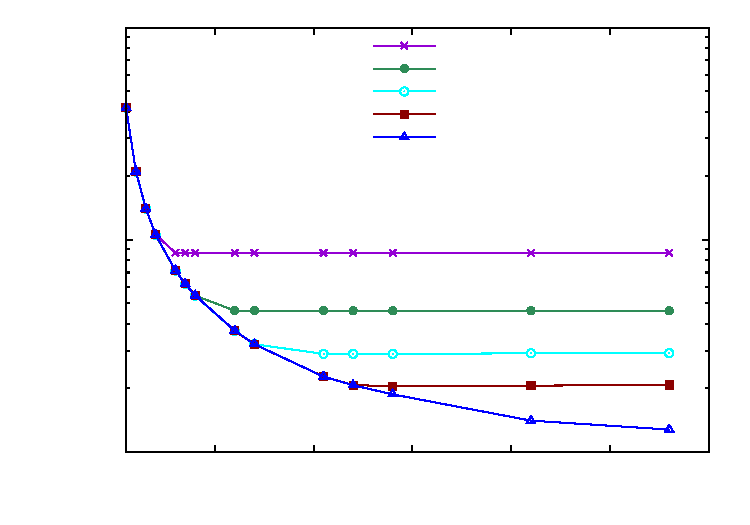
\includegraphics{plot-Tc_nogatherInt_00_500_selected_168}}%
    \gplfronttext
  \end{picture}%
\endgroup
}
      \caption{Tempo di completamento dell implementazione UDN con M=168 al variare del tempo di interarrivo}
      \label{fig:scalability_UDN_size168}
    \end{subfigure}
    ~
    \begin{subfigure}[b]{\textwidth}
      \centering
      \addtocounter{subfigure}{-1}
      \renewcommand\thesubfigure{\alph{subfigure}3}
      \resizebox{\columnwidth}{!}{% GNUPLOT: LaTeX picture with Postscript
\begingroup
  \makeatletter
  \providecommand\color[2][]{%
    \GenericError{(gnuplot) \space\space\space\@spaces}{%
      Package color not loaded in conjunction with
      terminal option `colourtext'%
    }{See the gnuplot documentation for explanation.%
    }{Either use 'blacktext' in gnuplot or load the package
      color.sty in LaTeX.}%
    \renewcommand\color[2][]{}%
  }%
  \providecommand\includegraphics[2][]{%
    \GenericError{(gnuplot) \space\space\space\@spaces}{%
      Package graphicx or graphics not loaded%
    }{See the gnuplot documentation for explanation.%
    }{The gnuplot epslatex terminal needs graphicx.sty or graphics.sty.}%
    \renewcommand\includegraphics[2][]{}%
  }%
  \providecommand\rotatebox[2]{#2}%
  \@ifundefined{ifGPcolor}{%
    \newif\ifGPcolor
    \GPcolortrue
  }{}%
  \@ifundefined{ifGPblacktext}{%
    \newif\ifGPblacktext
    \GPblacktexttrue
  }{}%
  % define a \g@addto@macro without @ in the name:
  \let\gplgaddtomacro\g@addto@macro
  % define empty templates for all commands taking text:
  \gdef\gplbacktext{}%
  \gdef\gplfronttext{}%
  \makeatother
  \ifGPblacktext
    % no textcolor at all
    \def\colorrgb#1{}%
    \def\colorgray#1{}%
  \else
    % gray or color?
    \ifGPcolor
      \def\colorrgb#1{\color[rgb]{#1}}%
      \def\colorgray#1{\color[gray]{#1}}%
      \expandafter\def\csname LTw\endcsname{\color{white}}%
      \expandafter\def\csname LTb\endcsname{\color{black}}%
      \expandafter\def\csname LTa\endcsname{\color{black}}%
      \expandafter\def\csname LT0\endcsname{\color[rgb]{1,0,0}}%
      \expandafter\def\csname LT1\endcsname{\color[rgb]{0,1,0}}%
      \expandafter\def\csname LT2\endcsname{\color[rgb]{0,0,1}}%
      \expandafter\def\csname LT3\endcsname{\color[rgb]{1,0,1}}%
      \expandafter\def\csname LT4\endcsname{\color[rgb]{0,1,1}}%
      \expandafter\def\csname LT5\endcsname{\color[rgb]{1,1,0}}%
      \expandafter\def\csname LT6\endcsname{\color[rgb]{0,0,0}}%
      \expandafter\def\csname LT7\endcsname{\color[rgb]{1,0.3,0}}%
      \expandafter\def\csname LT8\endcsname{\color[rgb]{0.5,0.5,0.5}}%
    \else
      % gray
      \def\colorrgb#1{\color{black}}%
      \def\colorgray#1{\color[gray]{#1}}%
      \expandafter\def\csname LTw\endcsname{\color{white}}%
      \expandafter\def\csname LTb\endcsname{\color{black}}%
      \expandafter\def\csname LTa\endcsname{\color{black}}%
      \expandafter\def\csname LT0\endcsname{\color{black}}%
      \expandafter\def\csname LT1\endcsname{\color{black}}%
      \expandafter\def\csname LT2\endcsname{\color{black}}%
      \expandafter\def\csname LT3\endcsname{\color{black}}%
      \expandafter\def\csname LT4\endcsname{\color{black}}%
      \expandafter\def\csname LT5\endcsname{\color{black}}%
      \expandafter\def\csname LT6\endcsname{\color{black}}%
      \expandafter\def\csname LT7\endcsname{\color{black}}%
      \expandafter\def\csname LT8\endcsname{\color{black}}%
    \fi
  \fi
  \setlength{\unitlength}{0.0500bp}%
  \begin{picture}(7200.00,5040.00)%
    \gplgaddtomacro\gplbacktext{%
      \csname LTb\endcsname%
      \put(1210,704){\makebox(0,0)[r]{\strut{} 10}}%
      \put(1210,2061){\makebox(0,0)[r]{\strut{} 100}}%
      \put(1210,3418){\makebox(0,0)[r]{\strut{} 1000}}%
      \put(1210,4775){\makebox(0,0)[r]{\strut{} 10000}}%
      \put(2175,484){\makebox(0,0){\strut{} 10}}%
      \put(3101,484){\makebox(0,0){\strut{} 20}}%
      \put(4026,484){\makebox(0,0){\strut{} 30}}%
      \put(4952,484){\makebox(0,0){\strut{} 40}}%
      \put(5877,484){\makebox(0,0){\strut{} 50}}%
      \put(6803,484){\makebox(0,0){\strut{} 60}}%
      \put(176,2739){\rotatebox{-270}{\makebox(0,0){\strut{}$T_{\textrm{C}}$ complete time (ms)}}}%
      \put(4072,154){\makebox(0,0){\strut{}parallel degree}}%
    }%
    \gplgaddtomacro\gplfronttext{%
      \csname LTb\endcsname%
      \put(3586,4602){\makebox(0,0)[r]{\strut{}$T_A$ 289.156 $\mu\mathrm{sec}$}}%
      \csname LTb\endcsname%
      \put(3586,4382){\makebox(0,0)[r]{\strut{}$T_A$ 173.494 $\mu\mathrm{sec}$}}%
      \csname LTb\endcsname%
      \put(3586,4162){\makebox(0,0)[r]{\strut{}$T_A$ 115.663 $\mu\mathrm{sec}$}}%
      \csname LTb\endcsname%
      \put(3586,3942){\makebox(0,0)[r]{\strut{}$T_A$ 92.530 $\mu\mathrm{sec}$}}%
      \csname LTb\endcsname%
      \put(3586,3722){\makebox(0,0)[r]{\strut{}$T_A$ 57.831 $\mu\mathrm{sec}$}}%
    }%
    \gplbacktext
    \put(0,0){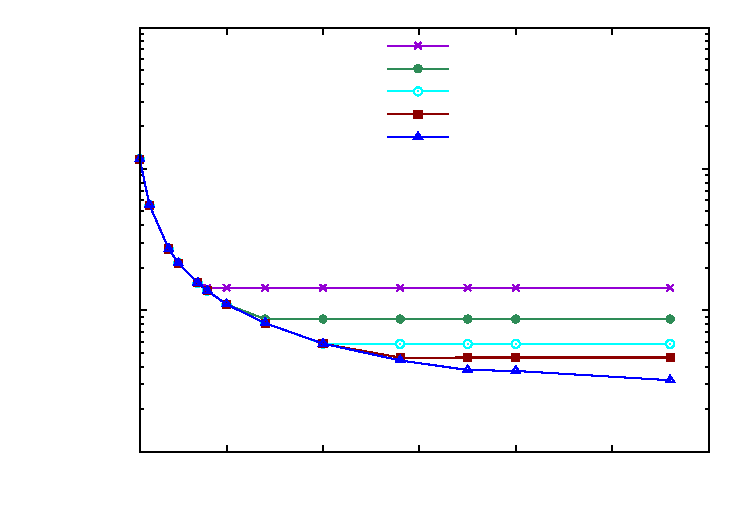
\includegraphics{plot-Tc_nogatherInt_00_500_selected_280}}%
    \gplfronttext
  \end{picture}%
\endgroup
}
      \caption{Tempo di completamento dell implementazione UDN con M=280 al variare del tempo di interarrivo}
      \label{fig:scalability_UDN_size280}
    \end{subfigure}
    \label{fig:allScalbility_UDN}
  \end{subfigure}
  \hspace{2ex}
  \begin{subfigure}[b]{.5\columnwidth}
    \centering
    \renewcommand\thesubfigure{\alph{subfigure}}
    \caption{Implementazione con solo SM}
    \begin{subfigure}[b]{\textwidth}
      \centering
      \addtocounter{subfigure}{-1}
      \renewcommand\thesubfigure{\alph{subfigure}1}
      \resizebox{\columnwidth}{!}{% GNUPLOT: LaTeX picture with Postscript
\begingroup
  \makeatletter
  \providecommand\color[2][]{%
    \GenericError{(gnuplot) \space\space\space\@spaces}{%
      Package color not loaded in conjunction with
      terminal option `colourtext'%
    }{See the gnuplot documentation for explanation.%
    }{Either use 'blacktext' in gnuplot or load the package
      color.sty in LaTeX.}%
    \renewcommand\color[2][]{}%
  }%
  \providecommand\includegraphics[2][]{%
    \GenericError{(gnuplot) \space\space\space\@spaces}{%
      Package graphicx or graphics not loaded%
    }{See the gnuplot documentation for explanation.%
    }{The gnuplot epslatex terminal needs graphicx.sty or graphics.sty.}%
    \renewcommand\includegraphics[2][]{}%
  }%
  \providecommand\rotatebox[2]{#2}%
  \@ifundefined{ifGPcolor}{%
    \newif\ifGPcolor
    \GPcolortrue
  }{}%
  \@ifundefined{ifGPblacktext}{%
    \newif\ifGPblacktext
    \GPblacktexttrue
  }{}%
  % define a \g@addto@macro without @ in the name:
  \let\gplgaddtomacro\g@addto@macro
  % define empty templates for all commands taking text:
  \gdef\gplbacktext{}%
  \gdef\gplfronttext{}%
  \makeatother
  \ifGPblacktext
    % no textcolor at all
    \def\colorrgb#1{}%
    \def\colorgray#1{}%
  \else
    % gray or color?
    \ifGPcolor
      \def\colorrgb#1{\color[rgb]{#1}}%
      \def\colorgray#1{\color[gray]{#1}}%
      \expandafter\def\csname LTw\endcsname{\color{white}}%
      \expandafter\def\csname LTb\endcsname{\color{black}}%
      \expandafter\def\csname LTa\endcsname{\color{black}}%
      \expandafter\def\csname LT0\endcsname{\color[rgb]{1,0,0}}%
      \expandafter\def\csname LT1\endcsname{\color[rgb]{0,1,0}}%
      \expandafter\def\csname LT2\endcsname{\color[rgb]{0,0,1}}%
      \expandafter\def\csname LT3\endcsname{\color[rgb]{1,0,1}}%
      \expandafter\def\csname LT4\endcsname{\color[rgb]{0,1,1}}%
      \expandafter\def\csname LT5\endcsname{\color[rgb]{1,1,0}}%
      \expandafter\def\csname LT6\endcsname{\color[rgb]{0,0,0}}%
      \expandafter\def\csname LT7\endcsname{\color[rgb]{1,0.3,0}}%
      \expandafter\def\csname LT8\endcsname{\color[rgb]{0.5,0.5,0.5}}%
    \else
      % gray
      \def\colorrgb#1{\color{black}}%
      \def\colorgray#1{\color[gray]{#1}}%
      \expandafter\def\csname LTw\endcsname{\color{white}}%
      \expandafter\def\csname LTb\endcsname{\color{black}}%
      \expandafter\def\csname LTa\endcsname{\color{black}}%
      \expandafter\def\csname LT0\endcsname{\color{black}}%
      \expandafter\def\csname LT1\endcsname{\color{black}}%
      \expandafter\def\csname LT2\endcsname{\color{black}}%
      \expandafter\def\csname LT3\endcsname{\color{black}}%
      \expandafter\def\csname LT4\endcsname{\color{black}}%
      \expandafter\def\csname LT5\endcsname{\color{black}}%
      \expandafter\def\csname LT6\endcsname{\color{black}}%
      \expandafter\def\csname LT7\endcsname{\color{black}}%
      \expandafter\def\csname LT8\endcsname{\color{black}}%
    \fi
  \fi
  \setlength{\unitlength}{0.0500bp}%
  \begin{picture}(7200.00,5040.00)%
    \gplgaddtomacro\gplbacktext{%
      \csname LTb\endcsname%
      \put(946,704){\makebox(0,0)[r]{\strut{} 1}}%
      \put(946,2740){\makebox(0,0)[r]{\strut{} 10}}%
      \put(946,4775){\makebox(0,0)[r]{\strut{} 100}}%
      \put(1951,484){\makebox(0,0){\strut{} 10}}%
      \put(2922,484){\makebox(0,0){\strut{} 20}}%
      \put(3892,484){\makebox(0,0){\strut{} 30}}%
      \put(4862,484){\makebox(0,0){\strut{} 40}}%
      \put(5833,484){\makebox(0,0){\strut{} 50}}%
      \put(6803,484){\makebox(0,0){\strut{} 60}}%
      \put(176,2739){\rotatebox{-270}{\makebox(0,0){\strut{}$T_{\textrm{C}}$ complete time (ms)}}}%
      \put(3940,154){\makebox(0,0){\strut{}parallel degree}}%
    }%
    \gplgaddtomacro\gplfronttext{%
      \csname LTb\endcsname%
      \put(3190,4602){\makebox(0,0)[r]{\strut{}$T_A$ 23.133 $\mu\mathrm{sec}$}}%
      \csname LTb\endcsname%
      \put(3190,4382){\makebox(0,0)[r]{\strut{}$T_A$ 11.566 $\mu\mathrm{sec}$}}%
      \csname LTb\endcsname%
      \put(3190,4162){\makebox(0,0)[r]{\strut{}$T_A$ 8.096 $\mu\mathrm{sec}$}}%
      \csname LTb\endcsname%
      \put(3190,3942){\makebox(0,0)[r]{\strut{}$T_A$ 4.627 $\mu\mathrm{sec}$}}%
    }%
    \gplbacktext
    \put(0,0){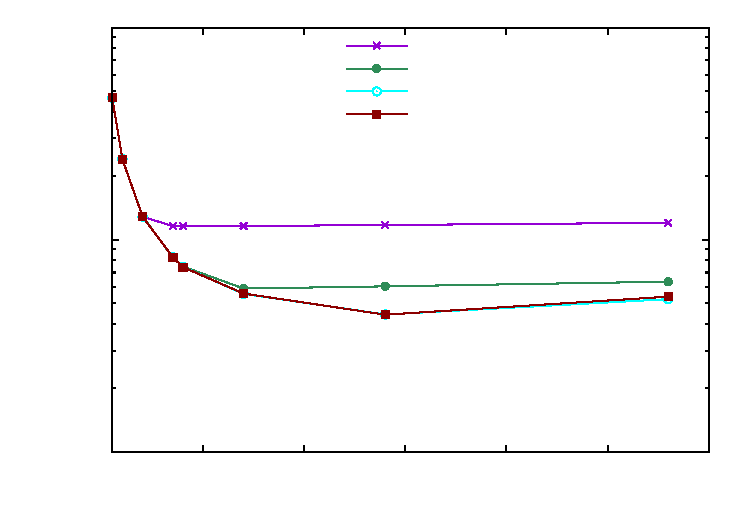
\includegraphics{plot-Tc_nogatherInt_11_500_selected_56}}%
    \gplfronttext
  \end{picture}%
\endgroup
}
      \caption{Tempo di completamento dell implementazione SM con M=56 al variare del tempo di interarrivo}
      \label{fig:scalability_SM_size56}
    \end{subfigure}
    ~
    \begin{subfigure}[b]{\textwidth}
      \centering
      \addtocounter{subfigure}{-1}
      \renewcommand\thesubfigure{\alph{subfigure}2}
      \resizebox{\columnwidth}{!}{% GNUPLOT: LaTeX picture with Postscript
\begingroup
  \makeatletter
  \providecommand\color[2][]{%
    \GenericError{(gnuplot) \space\space\space\@spaces}{%
      Package color not loaded in conjunction with
      terminal option `colourtext'%
    }{See the gnuplot documentation for explanation.%
    }{Either use 'blacktext' in gnuplot or load the package
      color.sty in LaTeX.}%
    \renewcommand\color[2][]{}%
  }%
  \providecommand\includegraphics[2][]{%
    \GenericError{(gnuplot) \space\space\space\@spaces}{%
      Package graphicx or graphics not loaded%
    }{See the gnuplot documentation for explanation.%
    }{The gnuplot epslatex terminal needs graphicx.sty or graphics.sty.}%
    \renewcommand\includegraphics[2][]{}%
  }%
  \providecommand\rotatebox[2]{#2}%
  \@ifundefined{ifGPcolor}{%
    \newif\ifGPcolor
    \GPcolortrue
  }{}%
  \@ifundefined{ifGPblacktext}{%
    \newif\ifGPblacktext
    \GPblacktexttrue
  }{}%
  % define a \g@addto@macro without @ in the name:
  \let\gplgaddtomacro\g@addto@macro
  % define empty templates for all commands taking text:
  \gdef\gplbacktext{}%
  \gdef\gplfronttext{}%
  \makeatother
  \ifGPblacktext
    % no textcolor at all
    \def\colorrgb#1{}%
    \def\colorgray#1{}%
  \else
    % gray or color?
    \ifGPcolor
      \def\colorrgb#1{\color[rgb]{#1}}%
      \def\colorgray#1{\color[gray]{#1}}%
      \expandafter\def\csname LTw\endcsname{\color{white}}%
      \expandafter\def\csname LTb\endcsname{\color{black}}%
      \expandafter\def\csname LTa\endcsname{\color{black}}%
      \expandafter\def\csname LT0\endcsname{\color[rgb]{1,0,0}}%
      \expandafter\def\csname LT1\endcsname{\color[rgb]{0,1,0}}%
      \expandafter\def\csname LT2\endcsname{\color[rgb]{0,0,1}}%
      \expandafter\def\csname LT3\endcsname{\color[rgb]{1,0,1}}%
      \expandafter\def\csname LT4\endcsname{\color[rgb]{0,1,1}}%
      \expandafter\def\csname LT5\endcsname{\color[rgb]{1,1,0}}%
      \expandafter\def\csname LT6\endcsname{\color[rgb]{0,0,0}}%
      \expandafter\def\csname LT7\endcsname{\color[rgb]{1,0.3,0}}%
      \expandafter\def\csname LT8\endcsname{\color[rgb]{0.5,0.5,0.5}}%
    \else
      % gray
      \def\colorrgb#1{\color{black}}%
      \def\colorgray#1{\color[gray]{#1}}%
      \expandafter\def\csname LTw\endcsname{\color{white}}%
      \expandafter\def\csname LTb\endcsname{\color{black}}%
      \expandafter\def\csname LTa\endcsname{\color{black}}%
      \expandafter\def\csname LT0\endcsname{\color{black}}%
      \expandafter\def\csname LT1\endcsname{\color{black}}%
      \expandafter\def\csname LT2\endcsname{\color{black}}%
      \expandafter\def\csname LT3\endcsname{\color{black}}%
      \expandafter\def\csname LT4\endcsname{\color{black}}%
      \expandafter\def\csname LT5\endcsname{\color{black}}%
      \expandafter\def\csname LT6\endcsname{\color{black}}%
      \expandafter\def\csname LT7\endcsname{\color{black}}%
      \expandafter\def\csname LT8\endcsname{\color{black}}%
    \fi
  \fi
  \setlength{\unitlength}{0.0500bp}%
  \begin{picture}(7200.00,5040.00)%
    \gplgaddtomacro\gplbacktext{%
      \csname LTb\endcsname%
      \put(1078,704){\makebox(0,0)[r]{\strut{} 10}}%
      \put(1078,2740){\makebox(0,0)[r]{\strut{} 100}}%
      \put(1078,4775){\makebox(0,0)[r]{\strut{} 1000}}%
      \put(2063,484){\makebox(0,0){\strut{} 10}}%
      \put(3011,484){\makebox(0,0){\strut{} 20}}%
      \put(3959,484){\makebox(0,0){\strut{} 30}}%
      \put(4907,484){\makebox(0,0){\strut{} 40}}%
      \put(5855,484){\makebox(0,0){\strut{} 50}}%
      \put(6803,484){\makebox(0,0){\strut{} 60}}%
      \put(176,2739){\rotatebox{-270}{\makebox(0,0){\strut{}$T_{\textrm{C}}$ complete time (ms)}}}%
      \put(4006,154){\makebox(0,0){\strut{}parallel degree}}%
    }%
    \gplgaddtomacro\gplfronttext{%
      \csname LTb\endcsname%
      \put(3454,4602){\makebox(0,0)[r]{\strut{}$T_A$ 173.494 $\mu\mathrm{sec}$}}%
      \csname LTb\endcsname%
      \put(3454,4382){\makebox(0,0)[r]{\strut{}$T_A$ 92.530 $\mu\mathrm{sec}$}}%
      \csname LTb\endcsname%
      \put(3454,4162){\makebox(0,0)[r]{\strut{}$T_A$ 57.831 $\mu\mathrm{sec}$}}%
      \csname LTb\endcsname%
      \put(3454,3942){\makebox(0,0)[r]{\strut{}$T_A$ 40.482 $\mu\mathrm{sec}$}}%
      \csname LTb\endcsname%
      \put(3454,3722){\makebox(0,0)[r]{\strut{}$T_A$ 23.133 $\mu\mathrm{sec}$}}%
    }%
    \gplbacktext
    \put(0,0){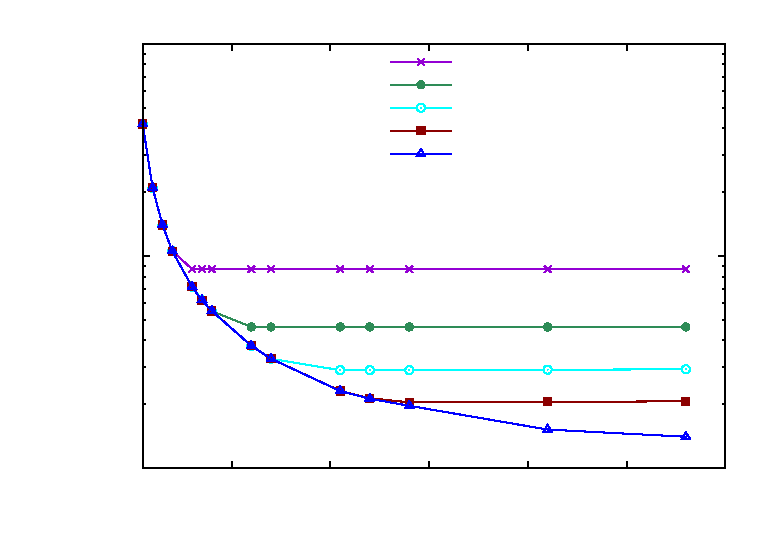
\includegraphics{plot-Tc_nogatherInt_11_500_selected_168}}%
    \gplfronttext
  \end{picture}%
\endgroup
}
      \caption{Tempo di completamento dell implementazione SM con M=168 al variare del tempo di interarrivo}
      \label{fig:scalability_SM_size168}
    \end{subfigure}
    ~
    \begin{subfigure}[b]{\textwidth}
      \centering
      \addtocounter{subfigure}{-1}
      \renewcommand\thesubfigure{\alph{subfigure}3}
      \resizebox{\columnwidth}{!}{% GNUPLOT: LaTeX picture with Postscript
\begingroup
  \makeatletter
  \providecommand\color[2][]{%
    \GenericError{(gnuplot) \space\space\space\@spaces}{%
      Package color not loaded in conjunction with
      terminal option `colourtext'%
    }{See the gnuplot documentation for explanation.%
    }{Either use 'blacktext' in gnuplot or load the package
      color.sty in LaTeX.}%
    \renewcommand\color[2][]{}%
  }%
  \providecommand\includegraphics[2][]{%
    \GenericError{(gnuplot) \space\space\space\@spaces}{%
      Package graphicx or graphics not loaded%
    }{See the gnuplot documentation for explanation.%
    }{The gnuplot epslatex terminal needs graphicx.sty or graphics.sty.}%
    \renewcommand\includegraphics[2][]{}%
  }%
  \providecommand\rotatebox[2]{#2}%
  \@ifundefined{ifGPcolor}{%
    \newif\ifGPcolor
    \GPcolortrue
  }{}%
  \@ifundefined{ifGPblacktext}{%
    \newif\ifGPblacktext
    \GPblacktexttrue
  }{}%
  % define a \g@addto@macro without @ in the name:
  \let\gplgaddtomacro\g@addto@macro
  % define empty templates for all commands taking text:
  \gdef\gplbacktext{}%
  \gdef\gplfronttext{}%
  \makeatother
  \ifGPblacktext
    % no textcolor at all
    \def\colorrgb#1{}%
    \def\colorgray#1{}%
  \else
    % gray or color?
    \ifGPcolor
      \def\colorrgb#1{\color[rgb]{#1}}%
      \def\colorgray#1{\color[gray]{#1}}%
      \expandafter\def\csname LTw\endcsname{\color{white}}%
      \expandafter\def\csname LTb\endcsname{\color{black}}%
      \expandafter\def\csname LTa\endcsname{\color{black}}%
      \expandafter\def\csname LT0\endcsname{\color[rgb]{1,0,0}}%
      \expandafter\def\csname LT1\endcsname{\color[rgb]{0,1,0}}%
      \expandafter\def\csname LT2\endcsname{\color[rgb]{0,0,1}}%
      \expandafter\def\csname LT3\endcsname{\color[rgb]{1,0,1}}%
      \expandafter\def\csname LT4\endcsname{\color[rgb]{0,1,1}}%
      \expandafter\def\csname LT5\endcsname{\color[rgb]{1,1,0}}%
      \expandafter\def\csname LT6\endcsname{\color[rgb]{0,0,0}}%
      \expandafter\def\csname LT7\endcsname{\color[rgb]{1,0.3,0}}%
      \expandafter\def\csname LT8\endcsname{\color[rgb]{0.5,0.5,0.5}}%
    \else
      % gray
      \def\colorrgb#1{\color{black}}%
      \def\colorgray#1{\color[gray]{#1}}%
      \expandafter\def\csname LTw\endcsname{\color{white}}%
      \expandafter\def\csname LTb\endcsname{\color{black}}%
      \expandafter\def\csname LTa\endcsname{\color{black}}%
      \expandafter\def\csname LT0\endcsname{\color{black}}%
      \expandafter\def\csname LT1\endcsname{\color{black}}%
      \expandafter\def\csname LT2\endcsname{\color{black}}%
      \expandafter\def\csname LT3\endcsname{\color{black}}%
      \expandafter\def\csname LT4\endcsname{\color{black}}%
      \expandafter\def\csname LT5\endcsname{\color{black}}%
      \expandafter\def\csname LT6\endcsname{\color{black}}%
      \expandafter\def\csname LT7\endcsname{\color{black}}%
      \expandafter\def\csname LT8\endcsname{\color{black}}%
    \fi
  \fi
  \setlength{\unitlength}{0.0500bp}%
  \begin{picture}(7200.00,5040.00)%
    \gplgaddtomacro\gplbacktext{%
      \csname LTb\endcsname%
      \put(1210,704){\makebox(0,0)[r]{\strut{} 10}}%
      \put(1210,2061){\makebox(0,0)[r]{\strut{} 100}}%
      \put(1210,3418){\makebox(0,0)[r]{\strut{} 1000}}%
      \put(1210,4775){\makebox(0,0)[r]{\strut{} 10000}}%
      \put(2175,484){\makebox(0,0){\strut{} 10}}%
      \put(3101,484){\makebox(0,0){\strut{} 20}}%
      \put(4026,484){\makebox(0,0){\strut{} 30}}%
      \put(4952,484){\makebox(0,0){\strut{} 40}}%
      \put(5877,484){\makebox(0,0){\strut{} 50}}%
      \put(6803,484){\makebox(0,0){\strut{} 60}}%
      \put(176,2739){\rotatebox{-270}{\makebox(0,0){\strut{}$T_{\textrm{C}}$ complete time (ms)}}}%
      \put(4072,154){\makebox(0,0){\strut{}parallel degree}}%
    }%
    \gplgaddtomacro\gplfronttext{%
      \csname LTb\endcsname%
      \put(3586,4602){\makebox(0,0)[r]{\strut{}$T_A$ 289.156 $\mu\mathrm{sec}$}}%
      \csname LTb\endcsname%
      \put(3586,4382){\makebox(0,0)[r]{\strut{}$T_A$ 173.494 $\mu\mathrm{sec}$}}%
      \csname LTb\endcsname%
      \put(3586,4162){\makebox(0,0)[r]{\strut{}$T_A$ 115.663 $\mu\mathrm{sec}$}}%
      \csname LTb\endcsname%
      \put(3586,3942){\makebox(0,0)[r]{\strut{}$T_A$ 92.530 $\mu\mathrm{sec}$}}%
      \csname LTb\endcsname%
      \put(3586,3722){\makebox(0,0)[r]{\strut{}$T_A$ 57.831 $\mu\mathrm{sec}$}}%
    }%
    \gplbacktext
    \put(0,0){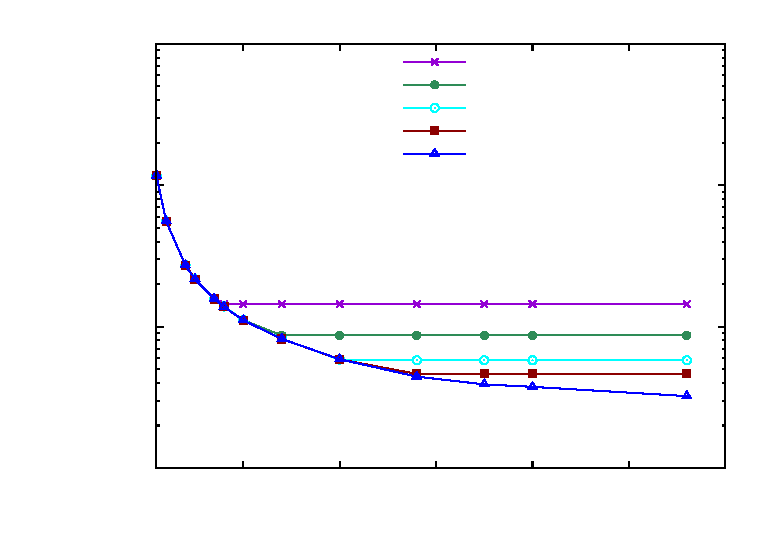
\includegraphics{plot-Tc_nogatherInt_11_500_selected_280}}%
    \gplfronttext
  \end{picture}%
\endgroup
}
      \caption{Tempo di completamento dell implementazione SM con M=280 al variare del tempo di interarrivo}
      \label{fig:scalability_SM_size280}
    \end{subfigure}
    \label{fig:allscalability_SM}
  \end{subfigure}
\end{figure}


%%%%%%%%%%%%%%%%%%%%%%%%%%%%%%%%%%%%%%%%%%%%%%%%%%%%%%%%%%%%%%%%%%%%%%%%%%%%%%%%

\newpage
%% \FloatBarrier
%% \subsection{Map service time} 

%% \begin{lstlisting}[morekeywords={servicet_stop, servicet_start, servicet_sum}]
%% void * generator_task(void *args...) {
%%   ...
%%   pthread_barrier_wait(...);
%%   for (i=0; i<m; i++) {
%%     a = get_clock_cycle();
%%     sym_send(ch_out, A_set[i]);
%%     while (get_clock_cycle() - a < Ta) 
%%       ;
%%   }
%%   ...
%% }

%% void * worker_task(void *args...) {
%%   ...
%%   servicet_stop = 0;
%%   pthread_barrier_wait(...);
%%   for (i=0; i<m; i++) {
%%     A = (int *)sym_receive(ch_in);
%%     atomic_compiler_barrier(); 
%%     if (rank == 0) {
%%       servicet_start = servicet_stop;
%%       servicet_stop = get_clock_cycle();
%%       if (servicet_start != 0)
%%         servicet_sum += servicet_stop - servicet_start;
%%     }
%%     atomic_compiler_barrier(); 
%%     if (ch_left != NULL) sym_send(ch_left, A);
%%     if (ch_right != NULL) sym_send(ch_right, A);
%%     for (j=0; j<g; j++) {
%%       C[j*rank] = 0;
%%       for (k=0; k<M; k++) 
%%         C[j*rank] = *(A+j*M+k) * B[k] + C[j*rank];
%%     }
%%     asymin_send(ch_out, C);
%%   }
%%   if (rank == 0)
%%     fprintf(output_file, ``%d %f\n'', n, (double)servicet_sum/m);
%%   ...
%% }

%% void * collector_task(void *args...) {
%%   ...
%%   pthread_barrier_wait(...);
%%   for (i=0; i<m; i++) {
%%     (void)asymin_receive(ch_in);
%%   }
%%   ...
%% }
%% \end{lstlisting}


\begin{figure}[p]
  \caption{Grafici di scalabilit\`a del tempo di servizio dello stream al variare del tempo di interarrivo}
  \begin{subfigure}[b]{.5\columnwidth}
    \centering
    \renewcommand\thesubfigure{\alph{subfigure}}
    %% se vuoi spostare questa caption in fondo devi modificare anche i contatori!
    \caption{Implementazione con solo UDN}
    \begin{subfigure}[b]{\textwidth}
      \centering
      \addtocounter{subfigure}{-1}
      \renewcommand\thesubfigure{\alph{subfigure}1}
      \resizebox{\columnwidth}{!}{% GNUPLOT: LaTeX picture with Postscript
\begingroup
  \makeatletter
  \providecommand\color[2][]{%
    \GenericError{(gnuplot) \space\space\space\@spaces}{%
      Package color not loaded in conjunction with
      terminal option `colourtext'%
    }{See the gnuplot documentation for explanation.%
    }{Either use 'blacktext' in gnuplot or load the package
      color.sty in LaTeX.}%
    \renewcommand\color[2][]{}%
  }%
  \providecommand\includegraphics[2][]{%
    \GenericError{(gnuplot) \space\space\space\@spaces}{%
      Package graphicx or graphics not loaded%
    }{See the gnuplot documentation for explanation.%
    }{The gnuplot epslatex terminal needs graphicx.sty or graphics.sty.}%
    \renewcommand\includegraphics[2][]{}%
  }%
  \providecommand\rotatebox[2]{#2}%
  \@ifundefined{ifGPcolor}{%
    \newif\ifGPcolor
    \GPcolortrue
  }{}%
  \@ifundefined{ifGPblacktext}{%
    \newif\ifGPblacktext
    \GPblacktexttrue
  }{}%
  % define a \g@addto@macro without @ in the name:
  \let\gplgaddtomacro\g@addto@macro
  % define empty templates for all commands taking text:
  \gdef\gplbacktext{}%
  \gdef\gplfronttext{}%
  \makeatother
  \ifGPblacktext
    % no textcolor at all
    \def\colorrgb#1{}%
    \def\colorgray#1{}%
  \else
    % gray or color?
    \ifGPcolor
      \def\colorrgb#1{\color[rgb]{#1}}%
      \def\colorgray#1{\color[gray]{#1}}%
      \expandafter\def\csname LTw\endcsname{\color{white}}%
      \expandafter\def\csname LTb\endcsname{\color{black}}%
      \expandafter\def\csname LTa\endcsname{\color{black}}%
      \expandafter\def\csname LT0\endcsname{\color[rgb]{1,0,0}}%
      \expandafter\def\csname LT1\endcsname{\color[rgb]{0,1,0}}%
      \expandafter\def\csname LT2\endcsname{\color[rgb]{0,0,1}}%
      \expandafter\def\csname LT3\endcsname{\color[rgb]{1,0,1}}%
      \expandafter\def\csname LT4\endcsname{\color[rgb]{0,1,1}}%
      \expandafter\def\csname LT5\endcsname{\color[rgb]{1,1,0}}%
      \expandafter\def\csname LT6\endcsname{\color[rgb]{0,0,0}}%
      \expandafter\def\csname LT7\endcsname{\color[rgb]{1,0.3,0}}%
      \expandafter\def\csname LT8\endcsname{\color[rgb]{0.5,0.5,0.5}}%
    \else
      % gray
      \def\colorrgb#1{\color{black}}%
      \def\colorgray#1{\color[gray]{#1}}%
      \expandafter\def\csname LTw\endcsname{\color{white}}%
      \expandafter\def\csname LTb\endcsname{\color{black}}%
      \expandafter\def\csname LTa\endcsname{\color{black}}%
      \expandafter\def\csname LT0\endcsname{\color{black}}%
      \expandafter\def\csname LT1\endcsname{\color{black}}%
      \expandafter\def\csname LT2\endcsname{\color{black}}%
      \expandafter\def\csname LT3\endcsname{\color{black}}%
      \expandafter\def\csname LT4\endcsname{\color{black}}%
      \expandafter\def\csname LT5\endcsname{\color{black}}%
      \expandafter\def\csname LT6\endcsname{\color{black}}%
      \expandafter\def\csname LT7\endcsname{\color{black}}%
      \expandafter\def\csname LT8\endcsname{\color{black}}%
    \fi
  \fi
  \setlength{\unitlength}{0.0500bp}%
  \begin{picture}(7200.00,5040.00)%
    \gplgaddtomacro\gplbacktext{%
      \csname LTb\endcsname%
      \put(814,1325){\makebox(0,0)[r]{\strut{} 10}}%
      \csname LTb\endcsname%
      \put(814,2015){\makebox(0,0)[r]{\strut{} 20}}%
      \csname LTb\endcsname%
      \put(814,2705){\makebox(0,0)[r]{\strut{} 30}}%
      \csname LTb\endcsname%
      \put(814,3395){\makebox(0,0)[r]{\strut{} 40}}%
      \csname LTb\endcsname%
      \put(814,4085){\makebox(0,0)[r]{\strut{} 50}}%
      \csname LTb\endcsname%
      \put(814,4775){\makebox(0,0)[r]{\strut{} 60}}%
      \csname LTb\endcsname%
      \put(1839,484){\makebox(0,0){\strut{} 10}}%
      \csname LTb\endcsname%
      \put(2832,484){\makebox(0,0){\strut{} 20}}%
      \csname LTb\endcsname%
      \put(3825,484){\makebox(0,0){\strut{} 30}}%
      \csname LTb\endcsname%
      \put(4818,484){\makebox(0,0){\strut{} 40}}%
      \csname LTb\endcsname%
      \put(5810,484){\makebox(0,0){\strut{} 50}}%
      \csname LTb\endcsname%
      \put(6803,484){\makebox(0,0){\strut{} 60}}%
      \put(176,2739){\rotatebox{-270}{\makebox(0,0){\strut{}scalability}}}%
      \put(3874,154){\makebox(0,0){\strut{}$n$ parallel degree}}%
    }%
    \gplgaddtomacro\gplfronttext{%
      \csname LTb\endcsname%
      \put(3322,4602){\makebox(0,0)[r]{\strut{}ideal scalability}}%
      \csname LTb\endcsname%
      \put(3322,4382){\makebox(0,0)[r]{\strut{}$T_A$ 20000 $\tau$}}%
      \csname LTb\endcsname%
      \put(3322,4162){\makebox(0,0)[r]{\strut{}$T_A$ 10000 $\tau$}}%
      \csname LTb\endcsname%
      \put(3322,3942){\makebox(0,0)[r]{\strut{}$T_A$ 7000 $\tau$}}%
      \csname LTb\endcsname%
      \put(3322,3722){\makebox(0,0)[r]{\strut{}$T_A$ 4000 $\tau$}}%
    }%
    \gplbacktext
    \put(0,0){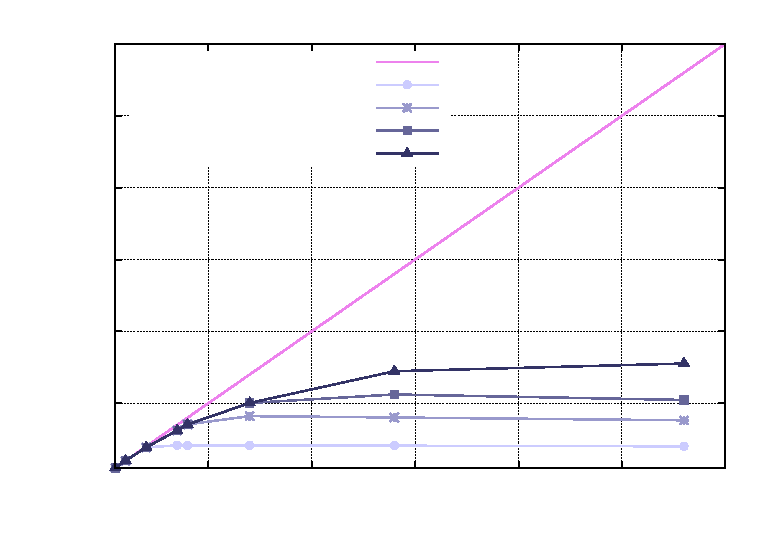
\includegraphics{plot-T-s_nogatherInt_00_500_selected_56}}%
    \gplfronttext
  \end{picture}%
\endgroup
}
      \caption{Scalabilit\`a dell'implementazione UDN con M=56 al variare del tempo di interarrivo}
      \label{fig:scalability_UDN_size56}
    \end{subfigure}
    ~
    \begin{subfigure}[b]{\textwidth}
      \centering
      \addtocounter{subfigure}{-1}
      \renewcommand\thesubfigure{\alph{subfigure}2}
      \resizebox{\columnwidth}{!}{% GNUPLOT: LaTeX picture with Postscript
\begingroup
  \makeatletter
  \providecommand\color[2][]{%
    \GenericError{(gnuplot) \space\space\space\@spaces}{%
      Package color not loaded in conjunction with
      terminal option `colourtext'%
    }{See the gnuplot documentation for explanation.%
    }{Either use 'blacktext' in gnuplot or load the package
      color.sty in LaTeX.}%
    \renewcommand\color[2][]{}%
  }%
  \providecommand\includegraphics[2][]{%
    \GenericError{(gnuplot) \space\space\space\@spaces}{%
      Package graphicx or graphics not loaded%
    }{See the gnuplot documentation for explanation.%
    }{The gnuplot epslatex terminal needs graphicx.sty or graphics.sty.}%
    \renewcommand\includegraphics[2][]{}%
  }%
  \providecommand\rotatebox[2]{#2}%
  \@ifundefined{ifGPcolor}{%
    \newif\ifGPcolor
    \GPcolortrue
  }{}%
  \@ifundefined{ifGPblacktext}{%
    \newif\ifGPblacktext
    \GPblacktexttrue
  }{}%
  % define a \g@addto@macro without @ in the name:
  \let\gplgaddtomacro\g@addto@macro
  % define empty templates for all commands taking text:
  \gdef\gplbacktext{}%
  \gdef\gplfronttext{}%
  \makeatother
  \ifGPblacktext
    % no textcolor at all
    \def\colorrgb#1{}%
    \def\colorgray#1{}%
  \else
    % gray or color?
    \ifGPcolor
      \def\colorrgb#1{\color[rgb]{#1}}%
      \def\colorgray#1{\color[gray]{#1}}%
      \expandafter\def\csname LTw\endcsname{\color{white}}%
      \expandafter\def\csname LTb\endcsname{\color{black}}%
      \expandafter\def\csname LTa\endcsname{\color{black}}%
      \expandafter\def\csname LT0\endcsname{\color[rgb]{1,0,0}}%
      \expandafter\def\csname LT1\endcsname{\color[rgb]{0,1,0}}%
      \expandafter\def\csname LT2\endcsname{\color[rgb]{0,0,1}}%
      \expandafter\def\csname LT3\endcsname{\color[rgb]{1,0,1}}%
      \expandafter\def\csname LT4\endcsname{\color[rgb]{0,1,1}}%
      \expandafter\def\csname LT5\endcsname{\color[rgb]{1,1,0}}%
      \expandafter\def\csname LT6\endcsname{\color[rgb]{0,0,0}}%
      \expandafter\def\csname LT7\endcsname{\color[rgb]{1,0.3,0}}%
      \expandafter\def\csname LT8\endcsname{\color[rgb]{0.5,0.5,0.5}}%
    \else
      % gray
      \def\colorrgb#1{\color{black}}%
      \def\colorgray#1{\color[gray]{#1}}%
      \expandafter\def\csname LTw\endcsname{\color{white}}%
      \expandafter\def\csname LTb\endcsname{\color{black}}%
      \expandafter\def\csname LTa\endcsname{\color{black}}%
      \expandafter\def\csname LT0\endcsname{\color{black}}%
      \expandafter\def\csname LT1\endcsname{\color{black}}%
      \expandafter\def\csname LT2\endcsname{\color{black}}%
      \expandafter\def\csname LT3\endcsname{\color{black}}%
      \expandafter\def\csname LT4\endcsname{\color{black}}%
      \expandafter\def\csname LT5\endcsname{\color{black}}%
      \expandafter\def\csname LT6\endcsname{\color{black}}%
      \expandafter\def\csname LT7\endcsname{\color{black}}%
      \expandafter\def\csname LT8\endcsname{\color{black}}%
    \fi
  \fi
  \setlength{\unitlength}{0.0500bp}%
  \begin{picture}(7200.00,5040.00)%
    \gplgaddtomacro\gplbacktext{%
      \csname LTb\endcsname%
      \put(814,1325){\makebox(0,0)[r]{\strut{} 10}}%
      \csname LTb\endcsname%
      \put(814,2015){\makebox(0,0)[r]{\strut{} 20}}%
      \csname LTb\endcsname%
      \put(814,2705){\makebox(0,0)[r]{\strut{} 30}}%
      \csname LTb\endcsname%
      \put(814,3395){\makebox(0,0)[r]{\strut{} 40}}%
      \csname LTb\endcsname%
      \put(814,4085){\makebox(0,0)[r]{\strut{} 50}}%
      \csname LTb\endcsname%
      \put(814,4775){\makebox(0,0)[r]{\strut{} 60}}%
      \csname LTb\endcsname%
      \put(1839,484){\makebox(0,0){\strut{} 10}}%
      \csname LTb\endcsname%
      \put(2832,484){\makebox(0,0){\strut{} 20}}%
      \csname LTb\endcsname%
      \put(3825,484){\makebox(0,0){\strut{} 30}}%
      \csname LTb\endcsname%
      \put(4818,484){\makebox(0,0){\strut{} 40}}%
      \csname LTb\endcsname%
      \put(5810,484){\makebox(0,0){\strut{} 50}}%
      \csname LTb\endcsname%
      \put(6803,484){\makebox(0,0){\strut{} 60}}%
      \put(176,2739){\rotatebox{-270}{\makebox(0,0){\strut{}scalability}}}%
      \put(3874,154){\makebox(0,0){\strut{}$n$ parallel degree}}%
    }%
    \gplgaddtomacro\gplfronttext{%
      \csname LTb\endcsname%
      \put(3322,4602){\makebox(0,0)[r]{\strut{}ideal scalability}}%
      \csname LTb\endcsname%
      \put(3322,4382){\makebox(0,0)[r]{\strut{}$T_A$ 150000 $\tau$}}%
      \csname LTb\endcsname%
      \put(3322,4162){\makebox(0,0)[r]{\strut{}$T_A$ 80000 $\tau$}}%
      \csname LTb\endcsname%
      \put(3322,3942){\makebox(0,0)[r]{\strut{}$T_A$ 50000 $\tau$}}%
      \csname LTb\endcsname%
      \put(3322,3722){\makebox(0,0)[r]{\strut{}$T_A$ 35000 $\tau$}}%
      \csname LTb\endcsname%
      \put(3322,3502){\makebox(0,0)[r]{\strut{}$T_A$ 20000 $\tau$}}%
    }%
    \gplbacktext
    \put(0,0){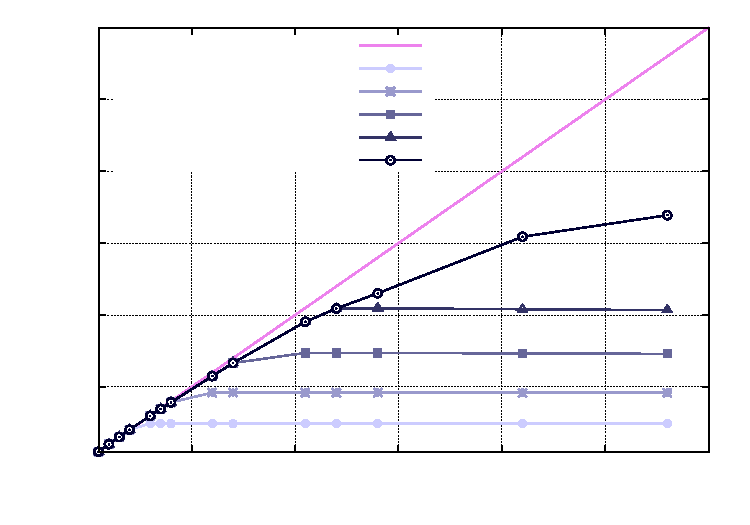
\includegraphics{plot-T-s_nogatherInt_00_500_selected_168}}%
    \gplfronttext
  \end{picture}%
\endgroup
}
      \caption{Scalabilit\`a dell'implementazione UDN con M=168 al variare del tempo di interarrivo}
      \label{fig:scalability_UDN_size168}
    \end{subfigure}
    ~
    \begin{subfigure}[b]{\textwidth}
      \centering
      \addtocounter{subfigure}{-1}
      \renewcommand\thesubfigure{\alph{subfigure}3}
      \resizebox{\columnwidth}{!}{% GNUPLOT: LaTeX picture with Postscript
\begingroup
  \makeatletter
  \providecommand\color[2][]{%
    \GenericError{(gnuplot) \space\space\space\@spaces}{%
      Package color not loaded in conjunction with
      terminal option `colourtext'%
    }{See the gnuplot documentation for explanation.%
    }{Either use 'blacktext' in gnuplot or load the package
      color.sty in LaTeX.}%
    \renewcommand\color[2][]{}%
  }%
  \providecommand\includegraphics[2][]{%
    \GenericError{(gnuplot) \space\space\space\@spaces}{%
      Package graphicx or graphics not loaded%
    }{See the gnuplot documentation for explanation.%
    }{The gnuplot epslatex terminal needs graphicx.sty or graphics.sty.}%
    \renewcommand\includegraphics[2][]{}%
  }%
  \providecommand\rotatebox[2]{#2}%
  \@ifundefined{ifGPcolor}{%
    \newif\ifGPcolor
    \GPcolortrue
  }{}%
  \@ifundefined{ifGPblacktext}{%
    \newif\ifGPblacktext
    \GPblacktexttrue
  }{}%
  % define a \g@addto@macro without @ in the name:
  \let\gplgaddtomacro\g@addto@macro
  % define empty templates for all commands taking text:
  \gdef\gplbacktext{}%
  \gdef\gplfronttext{}%
  \makeatother
  \ifGPblacktext
    % no textcolor at all
    \def\colorrgb#1{}%
    \def\colorgray#1{}%
  \else
    % gray or color?
    \ifGPcolor
      \def\colorrgb#1{\color[rgb]{#1}}%
      \def\colorgray#1{\color[gray]{#1}}%
      \expandafter\def\csname LTw\endcsname{\color{white}}%
      \expandafter\def\csname LTb\endcsname{\color{black}}%
      \expandafter\def\csname LTa\endcsname{\color{black}}%
      \expandafter\def\csname LT0\endcsname{\color[rgb]{1,0,0}}%
      \expandafter\def\csname LT1\endcsname{\color[rgb]{0,1,0}}%
      \expandafter\def\csname LT2\endcsname{\color[rgb]{0,0,1}}%
      \expandafter\def\csname LT3\endcsname{\color[rgb]{1,0,1}}%
      \expandafter\def\csname LT4\endcsname{\color[rgb]{0,1,1}}%
      \expandafter\def\csname LT5\endcsname{\color[rgb]{1,1,0}}%
      \expandafter\def\csname LT6\endcsname{\color[rgb]{0,0,0}}%
      \expandafter\def\csname LT7\endcsname{\color[rgb]{1,0.3,0}}%
      \expandafter\def\csname LT8\endcsname{\color[rgb]{0.5,0.5,0.5}}%
    \else
      % gray
      \def\colorrgb#1{\color{black}}%
      \def\colorgray#1{\color[gray]{#1}}%
      \expandafter\def\csname LTw\endcsname{\color{white}}%
      \expandafter\def\csname LTb\endcsname{\color{black}}%
      \expandafter\def\csname LTa\endcsname{\color{black}}%
      \expandafter\def\csname LT0\endcsname{\color{black}}%
      \expandafter\def\csname LT1\endcsname{\color{black}}%
      \expandafter\def\csname LT2\endcsname{\color{black}}%
      \expandafter\def\csname LT3\endcsname{\color{black}}%
      \expandafter\def\csname LT4\endcsname{\color{black}}%
      \expandafter\def\csname LT5\endcsname{\color{black}}%
      \expandafter\def\csname LT6\endcsname{\color{black}}%
      \expandafter\def\csname LT7\endcsname{\color{black}}%
      \expandafter\def\csname LT8\endcsname{\color{black}}%
    \fi
  \fi
  \setlength{\unitlength}{0.0500bp}%
  \begin{picture}(7200.00,5040.00)%
    \gplgaddtomacro\gplbacktext{%
      \csname LTb\endcsname%
      \put(814,1325){\makebox(0,0)[r]{\strut{} 10}}%
      \csname LTb\endcsname%
      \put(814,2015){\makebox(0,0)[r]{\strut{} 20}}%
      \csname LTb\endcsname%
      \put(814,2705){\makebox(0,0)[r]{\strut{} 30}}%
      \csname LTb\endcsname%
      \put(814,3395){\makebox(0,0)[r]{\strut{} 40}}%
      \csname LTb\endcsname%
      \put(814,4085){\makebox(0,0)[r]{\strut{} 50}}%
      \csname LTb\endcsname%
      \put(814,4775){\makebox(0,0)[r]{\strut{} 60}}%
      \csname LTb\endcsname%
      \put(1839,484){\makebox(0,0){\strut{} 10}}%
      \csname LTb\endcsname%
      \put(2832,484){\makebox(0,0){\strut{} 20}}%
      \csname LTb\endcsname%
      \put(3825,484){\makebox(0,0){\strut{} 30}}%
      \csname LTb\endcsname%
      \put(4818,484){\makebox(0,0){\strut{} 40}}%
      \csname LTb\endcsname%
      \put(5810,484){\makebox(0,0){\strut{} 50}}%
      \csname LTb\endcsname%
      \put(6803,484){\makebox(0,0){\strut{} 60}}%
      \put(176,2739){\rotatebox{-270}{\makebox(0,0){\strut{}scalability}}}%
      \put(3874,154){\makebox(0,0){\strut{}$n$ parallel degree}}%
    }%
    \gplgaddtomacro\gplfronttext{%
      \csname LTb\endcsname%
      \put(3322,4602){\makebox(0,0)[r]{\strut{}ideal scalability}}%
      \csname LTb\endcsname%
      \put(3322,4382){\makebox(0,0)[r]{\strut{}$T_A$ 250000 $\tau$}}%
      \csname LTb\endcsname%
      \put(3322,4162){\makebox(0,0)[r]{\strut{}$T_A$ 150000 $\tau$}}%
      \csname LTb\endcsname%
      \put(3322,3942){\makebox(0,0)[r]{\strut{}$T_A$ 100000 $\tau$}}%
      \csname LTb\endcsname%
      \put(3322,3722){\makebox(0,0)[r]{\strut{}$T_A$ 80000 $\tau$}}%
      \csname LTb\endcsname%
      \put(3322,3502){\makebox(0,0)[r]{\strut{}$T_A$ 50000 $\tau$}}%
    }%
    \gplbacktext
    \put(0,0){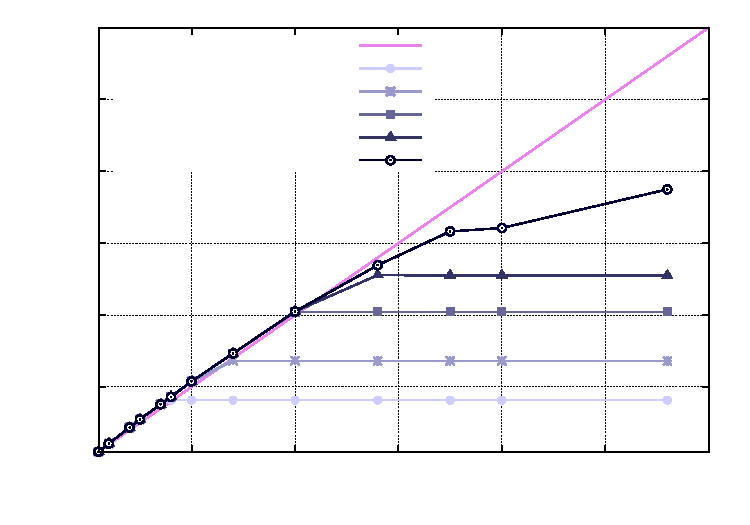
\includegraphics{plot-T-s_nogatherInt_00_500_selected_280}}%
    \gplfronttext
  \end{picture}%
\endgroup
}
      \caption{Scalabilit\`a dell'implementazione UDN con M=280 al variare del tempo di interarrivo}
      \label{fig:scalability_UDN_size280}
    \end{subfigure}
    \label{fig:allScalbility_UDN}
  \end{subfigure}
  \hspace{2ex}
  \begin{subfigure}[b]{.5\columnwidth}
    \centering
    \renewcommand\thesubfigure{\alph{subfigure}}
    \caption{Implementazione con solo SM}
    \begin{subfigure}[b]{\textwidth}
      \centering
      \addtocounter{subfigure}{-1}
      \renewcommand\thesubfigure{\alph{subfigure}1}
      \resizebox{\columnwidth}{!}{% GNUPLOT: LaTeX picture with Postscript
\begingroup
  \makeatletter
  \providecommand\color[2][]{%
    \GenericError{(gnuplot) \space\space\space\@spaces}{%
      Package color not loaded in conjunction with
      terminal option `colourtext'%
    }{See the gnuplot documentation for explanation.%
    }{Either use 'blacktext' in gnuplot or load the package
      color.sty in LaTeX.}%
    \renewcommand\color[2][]{}%
  }%
  \providecommand\includegraphics[2][]{%
    \GenericError{(gnuplot) \space\space\space\@spaces}{%
      Package graphicx or graphics not loaded%
    }{See the gnuplot documentation for explanation.%
    }{The gnuplot epslatex terminal needs graphicx.sty or graphics.sty.}%
    \renewcommand\includegraphics[2][]{}%
  }%
  \providecommand\rotatebox[2]{#2}%
  \@ifundefined{ifGPcolor}{%
    \newif\ifGPcolor
    \GPcolortrue
  }{}%
  \@ifundefined{ifGPblacktext}{%
    \newif\ifGPblacktext
    \GPblacktexttrue
  }{}%
  % define a \g@addto@macro without @ in the name:
  \let\gplgaddtomacro\g@addto@macro
  % define empty templates for all commands taking text:
  \gdef\gplbacktext{}%
  \gdef\gplfronttext{}%
  \makeatother
  \ifGPblacktext
    % no textcolor at all
    \def\colorrgb#1{}%
    \def\colorgray#1{}%
  \else
    % gray or color?
    \ifGPcolor
      \def\colorrgb#1{\color[rgb]{#1}}%
      \def\colorgray#1{\color[gray]{#1}}%
      \expandafter\def\csname LTw\endcsname{\color{white}}%
      \expandafter\def\csname LTb\endcsname{\color{black}}%
      \expandafter\def\csname LTa\endcsname{\color{black}}%
      \expandafter\def\csname LT0\endcsname{\color[rgb]{1,0,0}}%
      \expandafter\def\csname LT1\endcsname{\color[rgb]{0,1,0}}%
      \expandafter\def\csname LT2\endcsname{\color[rgb]{0,0,1}}%
      \expandafter\def\csname LT3\endcsname{\color[rgb]{1,0,1}}%
      \expandafter\def\csname LT4\endcsname{\color[rgb]{0,1,1}}%
      \expandafter\def\csname LT5\endcsname{\color[rgb]{1,1,0}}%
      \expandafter\def\csname LT6\endcsname{\color[rgb]{0,0,0}}%
      \expandafter\def\csname LT7\endcsname{\color[rgb]{1,0.3,0}}%
      \expandafter\def\csname LT8\endcsname{\color[rgb]{0.5,0.5,0.5}}%
    \else
      % gray
      \def\colorrgb#1{\color{black}}%
      \def\colorgray#1{\color[gray]{#1}}%
      \expandafter\def\csname LTw\endcsname{\color{white}}%
      \expandafter\def\csname LTb\endcsname{\color{black}}%
      \expandafter\def\csname LTa\endcsname{\color{black}}%
      \expandafter\def\csname LT0\endcsname{\color{black}}%
      \expandafter\def\csname LT1\endcsname{\color{black}}%
      \expandafter\def\csname LT2\endcsname{\color{black}}%
      \expandafter\def\csname LT3\endcsname{\color{black}}%
      \expandafter\def\csname LT4\endcsname{\color{black}}%
      \expandafter\def\csname LT5\endcsname{\color{black}}%
      \expandafter\def\csname LT6\endcsname{\color{black}}%
      \expandafter\def\csname LT7\endcsname{\color{black}}%
      \expandafter\def\csname LT8\endcsname{\color{black}}%
    \fi
  \fi
  \setlength{\unitlength}{0.0500bp}%
  \begin{picture}(7200.00,5040.00)%
    \gplgaddtomacro\gplbacktext{%
      \csname LTb\endcsname%
      \put(814,1325){\makebox(0,0)[r]{\strut{} 10}}%
      \csname LTb\endcsname%
      \put(814,2015){\makebox(0,0)[r]{\strut{} 20}}%
      \csname LTb\endcsname%
      \put(814,2705){\makebox(0,0)[r]{\strut{} 30}}%
      \csname LTb\endcsname%
      \put(814,3395){\makebox(0,0)[r]{\strut{} 40}}%
      \csname LTb\endcsname%
      \put(814,4085){\makebox(0,0)[r]{\strut{} 50}}%
      \csname LTb\endcsname%
      \put(814,4775){\makebox(0,0)[r]{\strut{} 60}}%
      \csname LTb\endcsname%
      \put(1839,484){\makebox(0,0){\strut{} 10}}%
      \csname LTb\endcsname%
      \put(2832,484){\makebox(0,0){\strut{} 20}}%
      \csname LTb\endcsname%
      \put(3825,484){\makebox(0,0){\strut{} 30}}%
      \csname LTb\endcsname%
      \put(4818,484){\makebox(0,0){\strut{} 40}}%
      \csname LTb\endcsname%
      \put(5810,484){\makebox(0,0){\strut{} 50}}%
      \csname LTb\endcsname%
      \put(6803,484){\makebox(0,0){\strut{} 60}}%
      \put(176,2739){\rotatebox{-270}{\makebox(0,0){\strut{}scalability}}}%
      \put(3874,154){\makebox(0,0){\strut{}$n$ parallel degree}}%
    }%
    \gplgaddtomacro\gplfronttext{%
      \csname LTb\endcsname%
      \put(3322,4602){\makebox(0,0)[r]{\strut{}ideal scalability}}%
      \csname LTb\endcsname%
      \put(3322,4382){\makebox(0,0)[r]{\strut{}$T_A$ 20000 $\tau$}}%
      \csname LTb\endcsname%
      \put(3322,4162){\makebox(0,0)[r]{\strut{}$T_A$ 10000 $\tau$}}%
      \csname LTb\endcsname%
      \put(3322,3942){\makebox(0,0)[r]{\strut{}$T_A$ 7000 $\tau$}}%
      \csname LTb\endcsname%
      \put(3322,3722){\makebox(0,0)[r]{\strut{}$T_A$ 4000 $\tau$}}%
    }%
    \gplbacktext
    \put(0,0){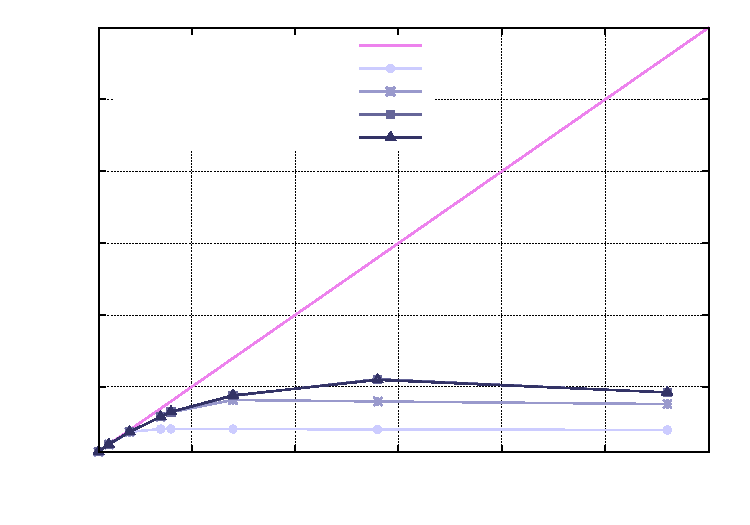
\includegraphics{plot-T-s_nogatherInt_11_500_selected_56}}%
    \gplfronttext
  \end{picture}%
\endgroup
}
      \caption{Scalabilit\`a dell'implementazione SM con M=56 al variare del tempo di interarrivo}
      \label{fig:scalability_SM_size56}
    \end{subfigure}
    ~
    \begin{subfigure}[b]{\textwidth}
      \centering
      \addtocounter{subfigure}{-1}
      \renewcommand\thesubfigure{\alph{subfigure}2}
      \resizebox{\columnwidth}{!}{% GNUPLOT: LaTeX picture with Postscript
\begingroup
  \makeatletter
  \providecommand\color[2][]{%
    \GenericError{(gnuplot) \space\space\space\@spaces}{%
      Package color not loaded in conjunction with
      terminal option `colourtext'%
    }{See the gnuplot documentation for explanation.%
    }{Either use 'blacktext' in gnuplot or load the package
      color.sty in LaTeX.}%
    \renewcommand\color[2][]{}%
  }%
  \providecommand\includegraphics[2][]{%
    \GenericError{(gnuplot) \space\space\space\@spaces}{%
      Package graphicx or graphics not loaded%
    }{See the gnuplot documentation for explanation.%
    }{The gnuplot epslatex terminal needs graphicx.sty or graphics.sty.}%
    \renewcommand\includegraphics[2][]{}%
  }%
  \providecommand\rotatebox[2]{#2}%
  \@ifundefined{ifGPcolor}{%
    \newif\ifGPcolor
    \GPcolortrue
  }{}%
  \@ifundefined{ifGPblacktext}{%
    \newif\ifGPblacktext
    \GPblacktexttrue
  }{}%
  % define a \g@addto@macro without @ in the name:
  \let\gplgaddtomacro\g@addto@macro
  % define empty templates for all commands taking text:
  \gdef\gplbacktext{}%
  \gdef\gplfronttext{}%
  \makeatother
  \ifGPblacktext
    % no textcolor at all
    \def\colorrgb#1{}%
    \def\colorgray#1{}%
  \else
    % gray or color?
    \ifGPcolor
      \def\colorrgb#1{\color[rgb]{#1}}%
      \def\colorgray#1{\color[gray]{#1}}%
      \expandafter\def\csname LTw\endcsname{\color{white}}%
      \expandafter\def\csname LTb\endcsname{\color{black}}%
      \expandafter\def\csname LTa\endcsname{\color{black}}%
      \expandafter\def\csname LT0\endcsname{\color[rgb]{1,0,0}}%
      \expandafter\def\csname LT1\endcsname{\color[rgb]{0,1,0}}%
      \expandafter\def\csname LT2\endcsname{\color[rgb]{0,0,1}}%
      \expandafter\def\csname LT3\endcsname{\color[rgb]{1,0,1}}%
      \expandafter\def\csname LT4\endcsname{\color[rgb]{0,1,1}}%
      \expandafter\def\csname LT5\endcsname{\color[rgb]{1,1,0}}%
      \expandafter\def\csname LT6\endcsname{\color[rgb]{0,0,0}}%
      \expandafter\def\csname LT7\endcsname{\color[rgb]{1,0.3,0}}%
      \expandafter\def\csname LT8\endcsname{\color[rgb]{0.5,0.5,0.5}}%
    \else
      % gray
      \def\colorrgb#1{\color{black}}%
      \def\colorgray#1{\color[gray]{#1}}%
      \expandafter\def\csname LTw\endcsname{\color{white}}%
      \expandafter\def\csname LTb\endcsname{\color{black}}%
      \expandafter\def\csname LTa\endcsname{\color{black}}%
      \expandafter\def\csname LT0\endcsname{\color{black}}%
      \expandafter\def\csname LT1\endcsname{\color{black}}%
      \expandafter\def\csname LT2\endcsname{\color{black}}%
      \expandafter\def\csname LT3\endcsname{\color{black}}%
      \expandafter\def\csname LT4\endcsname{\color{black}}%
      \expandafter\def\csname LT5\endcsname{\color{black}}%
      \expandafter\def\csname LT6\endcsname{\color{black}}%
      \expandafter\def\csname LT7\endcsname{\color{black}}%
      \expandafter\def\csname LT8\endcsname{\color{black}}%
    \fi
  \fi
  \setlength{\unitlength}{0.0500bp}%
  \begin{picture}(7200.00,5040.00)%
    \gplgaddtomacro\gplbacktext{%
      \csname LTb\endcsname%
      \put(814,1325){\makebox(0,0)[r]{\strut{} 10}}%
      \csname LTb\endcsname%
      \put(814,2015){\makebox(0,0)[r]{\strut{} 20}}%
      \csname LTb\endcsname%
      \put(814,2705){\makebox(0,0)[r]{\strut{} 30}}%
      \csname LTb\endcsname%
      \put(814,3395){\makebox(0,0)[r]{\strut{} 40}}%
      \csname LTb\endcsname%
      \put(814,4085){\makebox(0,0)[r]{\strut{} 50}}%
      \csname LTb\endcsname%
      \put(814,4775){\makebox(0,0)[r]{\strut{} 60}}%
      \csname LTb\endcsname%
      \put(1839,484){\makebox(0,0){\strut{} 10}}%
      \csname LTb\endcsname%
      \put(2832,484){\makebox(0,0){\strut{} 20}}%
      \csname LTb\endcsname%
      \put(3825,484){\makebox(0,0){\strut{} 30}}%
      \csname LTb\endcsname%
      \put(4818,484){\makebox(0,0){\strut{} 40}}%
      \csname LTb\endcsname%
      \put(5810,484){\makebox(0,0){\strut{} 50}}%
      \csname LTb\endcsname%
      \put(6803,484){\makebox(0,0){\strut{} 60}}%
      \put(176,2739){\rotatebox{-270}{\makebox(0,0){\strut{}scalability}}}%
      \put(3874,154){\makebox(0,0){\strut{}$n$ parallel degree}}%
    }%
    \gplgaddtomacro\gplfronttext{%
      \csname LTb\endcsname%
      \put(3322,4602){\makebox(0,0)[r]{\strut{}ideal scalability}}%
      \csname LTb\endcsname%
      \put(3322,4382){\makebox(0,0)[r]{\strut{}$T_A$ 150000 $\tau$}}%
      \csname LTb\endcsname%
      \put(3322,4162){\makebox(0,0)[r]{\strut{}$T_A$ 80000 $\tau$}}%
      \csname LTb\endcsname%
      \put(3322,3942){\makebox(0,0)[r]{\strut{}$T_A$ 50000 $\tau$}}%
      \csname LTb\endcsname%
      \put(3322,3722){\makebox(0,0)[r]{\strut{}$T_A$ 35000 $\tau$}}%
      \csname LTb\endcsname%
      \put(3322,3502){\makebox(0,0)[r]{\strut{}$T_A$ 20000 $\tau$}}%
    }%
    \gplbacktext
    \put(0,0){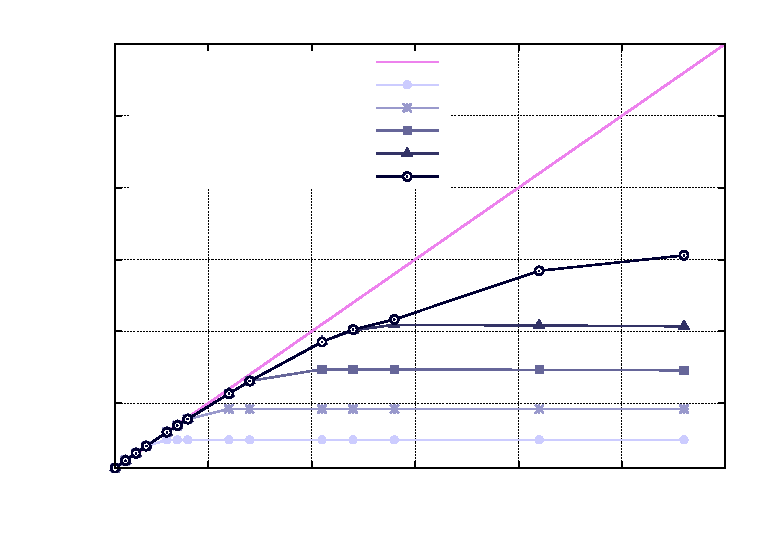
\includegraphics{plot-T-s_nogatherInt_11_500_selected_168}}%
    \gplfronttext
  \end{picture}%
\endgroup
}
      \caption{Scalabilit\`a dell'implementazione SM con M=168 al variare del tempo di interarrivo}
      \label{fig:scalability_SM_size168}
    \end{subfigure}
    ~
    \begin{subfigure}[b]{\textwidth}
      \centering
      \addtocounter{subfigure}{-1}
      \renewcommand\thesubfigure{\alph{subfigure}3}
      \resizebox{\columnwidth}{!}{% GNUPLOT: LaTeX picture with Postscript
\begingroup
  \makeatletter
  \providecommand\color[2][]{%
    \GenericError{(gnuplot) \space\space\space\@spaces}{%
      Package color not loaded in conjunction with
      terminal option `colourtext'%
    }{See the gnuplot documentation for explanation.%
    }{Either use 'blacktext' in gnuplot or load the package
      color.sty in LaTeX.}%
    \renewcommand\color[2][]{}%
  }%
  \providecommand\includegraphics[2][]{%
    \GenericError{(gnuplot) \space\space\space\@spaces}{%
      Package graphicx or graphics not loaded%
    }{See the gnuplot documentation for explanation.%
    }{The gnuplot epslatex terminal needs graphicx.sty or graphics.sty.}%
    \renewcommand\includegraphics[2][]{}%
  }%
  \providecommand\rotatebox[2]{#2}%
  \@ifundefined{ifGPcolor}{%
    \newif\ifGPcolor
    \GPcolortrue
  }{}%
  \@ifundefined{ifGPblacktext}{%
    \newif\ifGPblacktext
    \GPblacktexttrue
  }{}%
  % define a \g@addto@macro without @ in the name:
  \let\gplgaddtomacro\g@addto@macro
  % define empty templates for all commands taking text:
  \gdef\gplbacktext{}%
  \gdef\gplfronttext{}%
  \makeatother
  \ifGPblacktext
    % no textcolor at all
    \def\colorrgb#1{}%
    \def\colorgray#1{}%
  \else
    % gray or color?
    \ifGPcolor
      \def\colorrgb#1{\color[rgb]{#1}}%
      \def\colorgray#1{\color[gray]{#1}}%
      \expandafter\def\csname LTw\endcsname{\color{white}}%
      \expandafter\def\csname LTb\endcsname{\color{black}}%
      \expandafter\def\csname LTa\endcsname{\color{black}}%
      \expandafter\def\csname LT0\endcsname{\color[rgb]{1,0,0}}%
      \expandafter\def\csname LT1\endcsname{\color[rgb]{0,1,0}}%
      \expandafter\def\csname LT2\endcsname{\color[rgb]{0,0,1}}%
      \expandafter\def\csname LT3\endcsname{\color[rgb]{1,0,1}}%
      \expandafter\def\csname LT4\endcsname{\color[rgb]{0,1,1}}%
      \expandafter\def\csname LT5\endcsname{\color[rgb]{1,1,0}}%
      \expandafter\def\csname LT6\endcsname{\color[rgb]{0,0,0}}%
      \expandafter\def\csname LT7\endcsname{\color[rgb]{1,0.3,0}}%
      \expandafter\def\csname LT8\endcsname{\color[rgb]{0.5,0.5,0.5}}%
    \else
      % gray
      \def\colorrgb#1{\color{black}}%
      \def\colorgray#1{\color[gray]{#1}}%
      \expandafter\def\csname LTw\endcsname{\color{white}}%
      \expandafter\def\csname LTb\endcsname{\color{black}}%
      \expandafter\def\csname LTa\endcsname{\color{black}}%
      \expandafter\def\csname LT0\endcsname{\color{black}}%
      \expandafter\def\csname LT1\endcsname{\color{black}}%
      \expandafter\def\csname LT2\endcsname{\color{black}}%
      \expandafter\def\csname LT3\endcsname{\color{black}}%
      \expandafter\def\csname LT4\endcsname{\color{black}}%
      \expandafter\def\csname LT5\endcsname{\color{black}}%
      \expandafter\def\csname LT6\endcsname{\color{black}}%
      \expandafter\def\csname LT7\endcsname{\color{black}}%
      \expandafter\def\csname LT8\endcsname{\color{black}}%
    \fi
  \fi
  \setlength{\unitlength}{0.0500bp}%
  \begin{picture}(7200.00,5040.00)%
    \gplgaddtomacro\gplbacktext{%
      \csname LTb\endcsname%
      \put(814,1325){\makebox(0,0)[r]{\strut{} 10}}%
      \csname LTb\endcsname%
      \put(814,2015){\makebox(0,0)[r]{\strut{} 20}}%
      \csname LTb\endcsname%
      \put(814,2705){\makebox(0,0)[r]{\strut{} 30}}%
      \csname LTb\endcsname%
      \put(814,3395){\makebox(0,0)[r]{\strut{} 40}}%
      \csname LTb\endcsname%
      \put(814,4085){\makebox(0,0)[r]{\strut{} 50}}%
      \csname LTb\endcsname%
      \put(814,4775){\makebox(0,0)[r]{\strut{} 60}}%
      \csname LTb\endcsname%
      \put(1839,484){\makebox(0,0){\strut{} 10}}%
      \csname LTb\endcsname%
      \put(2832,484){\makebox(0,0){\strut{} 20}}%
      \csname LTb\endcsname%
      \put(3825,484){\makebox(0,0){\strut{} 30}}%
      \csname LTb\endcsname%
      \put(4818,484){\makebox(0,0){\strut{} 40}}%
      \csname LTb\endcsname%
      \put(5810,484){\makebox(0,0){\strut{} 50}}%
      \csname LTb\endcsname%
      \put(6803,484){\makebox(0,0){\strut{} 60}}%
      \put(176,2739){\rotatebox{-270}{\makebox(0,0){\strut{}scalability}}}%
      \put(3874,154){\makebox(0,0){\strut{}$n$ parallel degree}}%
    }%
    \gplgaddtomacro\gplfronttext{%
      \csname LTb\endcsname%
      \put(3322,4602){\makebox(0,0)[r]{\strut{}ideal scalability}}%
      \csname LTb\endcsname%
      \put(3322,4382){\makebox(0,0)[r]{\strut{}$T_A$ 250000 $\tau$}}%
      \csname LTb\endcsname%
      \put(3322,4162){\makebox(0,0)[r]{\strut{}$T_A$ 150000 $\tau$}}%
      \csname LTb\endcsname%
      \put(3322,3942){\makebox(0,0)[r]{\strut{}$T_A$ 100000 $\tau$}}%
      \csname LTb\endcsname%
      \put(3322,3722){\makebox(0,0)[r]{\strut{}$T_A$ 80000 $\tau$}}%
      \csname LTb\endcsname%
      \put(3322,3502){\makebox(0,0)[r]{\strut{}$T_A$ 50000 $\tau$}}%
    }%
    \gplbacktext
    \put(0,0){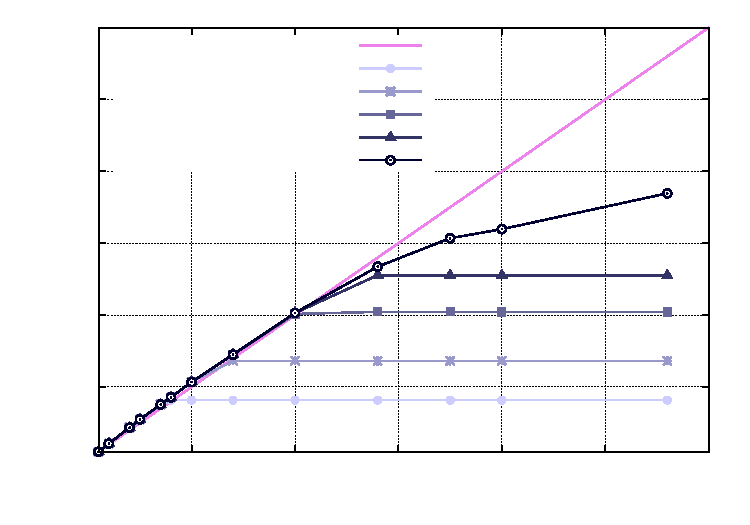
\includegraphics{plot-T-s_nogatherInt_11_500_selected_280}}%
    \gplfronttext
  \end{picture}%
\endgroup
}
      \caption{Scalabilit\`a dell'implementazione SM con M=280 al variare del tempo di interarrivo}
      \label{fig:scalability_SM_size280}
    \end{subfigure}
    \label{fig:allscalability_SM}
  \end{subfigure}
\end{figure}


%%%%%%%%%%%%%%%%%%%%%%%%%%%%%%%%%%%%%%%%%%%%%%%%%%%%%%%%%%%%%%%%%%%%%%%%%%%%%%%%


\begin{figure}[p]
  \caption{Grafici del tempo di servizio al variare del tempo di interarrivo}
  \begin{subfigure}[b]{.5\columnwidth}
    \centering
    \renewcommand\thesubfigure{\alph{subfigure}}
    %% se vuoi spostare questa caption in fondo devi modificare anche i contatori!
    \caption{Implementazione con solo UDN}
    \begin{subfigure}[b]{\textwidth}
      \centering
      \addtocounter{subfigure}{-1}
      \renewcommand\thesubfigure{\alph{subfigure}1}
      \resizebox{\columnwidth}{!}{% GNUPLOT: LaTeX picture with Postscript
\begingroup
  \makeatletter
  \providecommand\color[2][]{%
    \GenericError{(gnuplot) \space\space\space\@spaces}{%
      Package color not loaded in conjunction with
      terminal option `colourtext'%
    }{See the gnuplot documentation for explanation.%
    }{Either use 'blacktext' in gnuplot or load the package
      color.sty in LaTeX.}%
    \renewcommand\color[2][]{}%
  }%
  \providecommand\includegraphics[2][]{%
    \GenericError{(gnuplot) \space\space\space\@spaces}{%
      Package graphicx or graphics not loaded%
    }{See the gnuplot documentation for explanation.%
    }{The gnuplot epslatex terminal needs graphicx.sty or graphics.sty.}%
    \renewcommand\includegraphics[2][]{}%
  }%
  \providecommand\rotatebox[2]{#2}%
  \@ifundefined{ifGPcolor}{%
    \newif\ifGPcolor
    \GPcolortrue
  }{}%
  \@ifundefined{ifGPblacktext}{%
    \newif\ifGPblacktext
    \GPblacktexttrue
  }{}%
  % define a \g@addto@macro without @ in the name:
  \let\gplgaddtomacro\g@addto@macro
  % define empty templates for all commands taking text:
  \gdef\gplbacktext{}%
  \gdef\gplfronttext{}%
  \makeatother
  \ifGPblacktext
    % no textcolor at all
    \def\colorrgb#1{}%
    \def\colorgray#1{}%
  \else
    % gray or color?
    \ifGPcolor
      \def\colorrgb#1{\color[rgb]{#1}}%
      \def\colorgray#1{\color[gray]{#1}}%
      \expandafter\def\csname LTw\endcsname{\color{white}}%
      \expandafter\def\csname LTb\endcsname{\color{black}}%
      \expandafter\def\csname LTa\endcsname{\color{black}}%
      \expandafter\def\csname LT0\endcsname{\color[rgb]{1,0,0}}%
      \expandafter\def\csname LT1\endcsname{\color[rgb]{0,1,0}}%
      \expandafter\def\csname LT2\endcsname{\color[rgb]{0,0,1}}%
      \expandafter\def\csname LT3\endcsname{\color[rgb]{1,0,1}}%
      \expandafter\def\csname LT4\endcsname{\color[rgb]{0,1,1}}%
      \expandafter\def\csname LT5\endcsname{\color[rgb]{1,1,0}}%
      \expandafter\def\csname LT6\endcsname{\color[rgb]{0,0,0}}%
      \expandafter\def\csname LT7\endcsname{\color[rgb]{1,0.3,0}}%
      \expandafter\def\csname LT8\endcsname{\color[rgb]{0.5,0.5,0.5}}%
    \else
      % gray
      \def\colorrgb#1{\color{black}}%
      \def\colorgray#1{\color[gray]{#1}}%
      \expandafter\def\csname LTw\endcsname{\color{white}}%
      \expandafter\def\csname LTb\endcsname{\color{black}}%
      \expandafter\def\csname LTa\endcsname{\color{black}}%
      \expandafter\def\csname LT0\endcsname{\color{black}}%
      \expandafter\def\csname LT1\endcsname{\color{black}}%
      \expandafter\def\csname LT2\endcsname{\color{black}}%
      \expandafter\def\csname LT3\endcsname{\color{black}}%
      \expandafter\def\csname LT4\endcsname{\color{black}}%
      \expandafter\def\csname LT5\endcsname{\color{black}}%
      \expandafter\def\csname LT6\endcsname{\color{black}}%
      \expandafter\def\csname LT7\endcsname{\color{black}}%
      \expandafter\def\csname LT8\endcsname{\color{black}}%
    \fi
  \fi
  \setlength{\unitlength}{0.0500bp}%
  \begin{picture}(7200.00,5040.00)%
    \gplgaddtomacro\gplbacktext{%
      \csname LTb\endcsname%
      \put(1342,704){\makebox(0,0)[r]{\strut{} 1000}}%
      \put(1342,1722){\makebox(0,0)[r]{\strut{} 10000}}%
      \put(1342,2740){\makebox(0,0)[r]{\strut{} 100000}}%
      \put(1342,3757){\makebox(0,0)[r]{\strut{} 1e+06}}%
      \put(1342,4775){\makebox(0,0)[r]{\strut{} 1e+07}}%
      \put(2287,484){\makebox(0,0){\strut{} 10}}%
      \put(3190,484){\makebox(0,0){\strut{} 20}}%
      \put(4093,484){\makebox(0,0){\strut{} 30}}%
      \put(4997,484){\makebox(0,0){\strut{} 40}}%
      \put(5900,484){\makebox(0,0){\strut{} 50}}%
      \put(6803,484){\makebox(0,0){\strut{} 60}}%
      \put(176,2739){\rotatebox{-270}{\makebox(0,0){\strut{}service time ($\tau$)}}}%
      \put(4138,154){\makebox(0,0){\strut{}parallel degree}}%
    }%
    \gplgaddtomacro\gplfronttext{%
      \csname LTb\endcsname%
      \put(2926,4602){\makebox(0,0)[r]{\strut{}$T_A$ 20000 $\tau$}}%
      \csname LTb\endcsname%
      \put(2926,4382){\makebox(0,0)[r]{\strut{}$T_A$ 10000 $\tau$}}%
      \csname LTb\endcsname%
      \put(2926,4162){\makebox(0,0)[r]{\strut{}$T_A$ 7000 $\tau$}}%
      \csname LTb\endcsname%
      \put(2926,3942){\makebox(0,0)[r]{\strut{}$T_A$ 4000 $\tau$}}%
    }%
    \gplbacktext
    \put(0,0){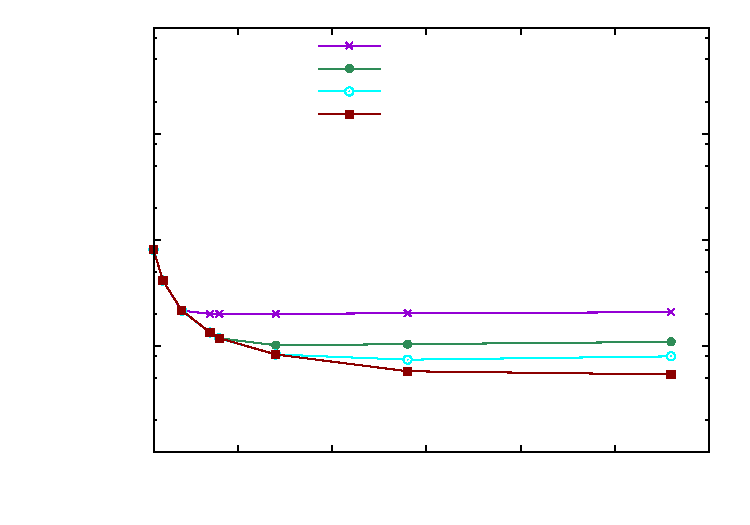
\includegraphics{plot-T_nogatherInt_00_500_selected_56}}%
    \gplfronttext
  \end{picture}%
\endgroup
}
      \caption{Tempo di servizio dell'implementazione UDN con M=56 al variare del tempo di interarrivo}
      \label{fig:scalability_UDN_size56}
    \end{subfigure}
    ~
    \begin{subfigure}[b]{\textwidth}
      \centering
      \addtocounter{subfigure}{-1}
      \renewcommand\thesubfigure{\alph{subfigure}2}
      \resizebox{\columnwidth}{!}{% GNUPLOT: LaTeX picture with Postscript
\begingroup
  \makeatletter
  \providecommand\color[2][]{%
    \GenericError{(gnuplot) \space\space\space\@spaces}{%
      Package color not loaded in conjunction with
      terminal option `colourtext'%
    }{See the gnuplot documentation for explanation.%
    }{Either use 'blacktext' in gnuplot or load the package
      color.sty in LaTeX.}%
    \renewcommand\color[2][]{}%
  }%
  \providecommand\includegraphics[2][]{%
    \GenericError{(gnuplot) \space\space\space\@spaces}{%
      Package graphicx or graphics not loaded%
    }{See the gnuplot documentation for explanation.%
    }{The gnuplot epslatex terminal needs graphicx.sty or graphics.sty.}%
    \renewcommand\includegraphics[2][]{}%
  }%
  \providecommand\rotatebox[2]{#2}%
  \@ifundefined{ifGPcolor}{%
    \newif\ifGPcolor
    \GPcolortrue
  }{}%
  \@ifundefined{ifGPblacktext}{%
    \newif\ifGPblacktext
    \GPblacktexttrue
  }{}%
  % define a \g@addto@macro without @ in the name:
  \let\gplgaddtomacro\g@addto@macro
  % define empty templates for all commands taking text:
  \gdef\gplbacktext{}%
  \gdef\gplfronttext{}%
  \makeatother
  \ifGPblacktext
    % no textcolor at all
    \def\colorrgb#1{}%
    \def\colorgray#1{}%
  \else
    % gray or color?
    \ifGPcolor
      \def\colorrgb#1{\color[rgb]{#1}}%
      \def\colorgray#1{\color[gray]{#1}}%
      \expandafter\def\csname LTw\endcsname{\color{white}}%
      \expandafter\def\csname LTb\endcsname{\color{black}}%
      \expandafter\def\csname LTa\endcsname{\color{black}}%
      \expandafter\def\csname LT0\endcsname{\color[rgb]{1,0,0}}%
      \expandafter\def\csname LT1\endcsname{\color[rgb]{0,1,0}}%
      \expandafter\def\csname LT2\endcsname{\color[rgb]{0,0,1}}%
      \expandafter\def\csname LT3\endcsname{\color[rgb]{1,0,1}}%
      \expandafter\def\csname LT4\endcsname{\color[rgb]{0,1,1}}%
      \expandafter\def\csname LT5\endcsname{\color[rgb]{1,1,0}}%
      \expandafter\def\csname LT6\endcsname{\color[rgb]{0,0,0}}%
      \expandafter\def\csname LT7\endcsname{\color[rgb]{1,0.3,0}}%
      \expandafter\def\csname LT8\endcsname{\color[rgb]{0.5,0.5,0.5}}%
    \else
      % gray
      \def\colorrgb#1{\color{black}}%
      \def\colorgray#1{\color[gray]{#1}}%
      \expandafter\def\csname LTw\endcsname{\color{white}}%
      \expandafter\def\csname LTb\endcsname{\color{black}}%
      \expandafter\def\csname LTa\endcsname{\color{black}}%
      \expandafter\def\csname LT0\endcsname{\color{black}}%
      \expandafter\def\csname LT1\endcsname{\color{black}}%
      \expandafter\def\csname LT2\endcsname{\color{black}}%
      \expandafter\def\csname LT3\endcsname{\color{black}}%
      \expandafter\def\csname LT4\endcsname{\color{black}}%
      \expandafter\def\csname LT5\endcsname{\color{black}}%
      \expandafter\def\csname LT6\endcsname{\color{black}}%
      \expandafter\def\csname LT7\endcsname{\color{black}}%
      \expandafter\def\csname LT8\endcsname{\color{black}}%
    \fi
  \fi
  \setlength{\unitlength}{0.0500bp}%
  \begin{picture}(7200.00,5040.00)%
    \gplgaddtomacro\gplbacktext{%
      \csname LTb\endcsname%
      \put(1342,704){\makebox(0,0)[r]{\strut{} 1000}}%
      \put(1342,1722){\makebox(0,0)[r]{\strut{} 10000}}%
      \put(1342,2740){\makebox(0,0)[r]{\strut{} 100000}}%
      \put(1342,3757){\makebox(0,0)[r]{\strut{} 1e+06}}%
      \put(1342,4775){\makebox(0,0)[r]{\strut{} 1e+07}}%
      \put(2287,484){\makebox(0,0){\strut{} 10}}%
      \put(3190,484){\makebox(0,0){\strut{} 20}}%
      \put(4093,484){\makebox(0,0){\strut{} 30}}%
      \put(4997,484){\makebox(0,0){\strut{} 40}}%
      \put(5900,484){\makebox(0,0){\strut{} 50}}%
      \put(6803,484){\makebox(0,0){\strut{} 60}}%
      \put(176,2739){\rotatebox{-270}{\makebox(0,0){\strut{}service time ($\tau$)}}}%
      \put(4138,154){\makebox(0,0){\strut{}parallel degree}}%
    }%
    \gplgaddtomacro\gplfronttext{%
      \csname LTb\endcsname%
      \put(3058,4602){\makebox(0,0)[r]{\strut{}$T_A$ 150000 $\tau$}}%
      \csname LTb\endcsname%
      \put(3058,4382){\makebox(0,0)[r]{\strut{}$T_A$ 80000 $\tau$}}%
      \csname LTb\endcsname%
      \put(3058,4162){\makebox(0,0)[r]{\strut{}$T_A$ 50000 $\tau$}}%
      \csname LTb\endcsname%
      \put(3058,3942){\makebox(0,0)[r]{\strut{}$T_A$ 35000 $\tau$}}%
      \csname LTb\endcsname%
      \put(3058,3722){\makebox(0,0)[r]{\strut{}$T_A$ 20000 $\tau$}}%
    }%
    \gplbacktext
    \put(0,0){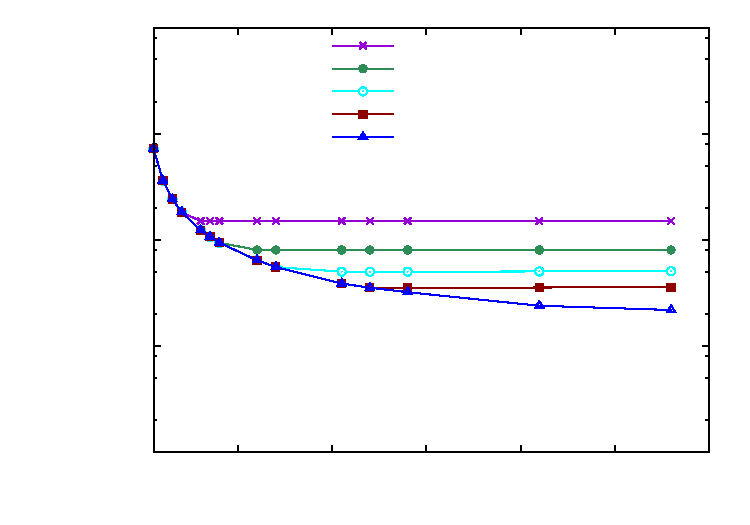
\includegraphics{plot-T_nogatherInt_00_500_selected_168}}%
    \gplfronttext
  \end{picture}%
\endgroup
}
      \caption{Tempo di servizio dell'implementazione UDN con M=168 al variare del tempo di interarrivo}
      \label{fig:scalability_UDN_size168}
    \end{subfigure}
    ~
    \begin{subfigure}[b]{\textwidth}
      \centering
      \addtocounter{subfigure}{-1}
      \renewcommand\thesubfigure{\alph{subfigure}3}
      \resizebox{\columnwidth}{!}{% GNUPLOT: LaTeX picture with Postscript
\begingroup
  \makeatletter
  \providecommand\color[2][]{%
    \GenericError{(gnuplot) \space\space\space\@spaces}{%
      Package color not loaded in conjunction with
      terminal option `colourtext'%
    }{See the gnuplot documentation for explanation.%
    }{Either use 'blacktext' in gnuplot or load the package
      color.sty in LaTeX.}%
    \renewcommand\color[2][]{}%
  }%
  \providecommand\includegraphics[2][]{%
    \GenericError{(gnuplot) \space\space\space\@spaces}{%
      Package graphicx or graphics not loaded%
    }{See the gnuplot documentation for explanation.%
    }{The gnuplot epslatex terminal needs graphicx.sty or graphics.sty.}%
    \renewcommand\includegraphics[2][]{}%
  }%
  \providecommand\rotatebox[2]{#2}%
  \@ifundefined{ifGPcolor}{%
    \newif\ifGPcolor
    \GPcolortrue
  }{}%
  \@ifundefined{ifGPblacktext}{%
    \newif\ifGPblacktext
    \GPblacktexttrue
  }{}%
  % define a \g@addto@macro without @ in the name:
  \let\gplgaddtomacro\g@addto@macro
  % define empty templates for all commands taking text:
  \gdef\gplbacktext{}%
  \gdef\gplfronttext{}%
  \makeatother
  \ifGPblacktext
    % no textcolor at all
    \def\colorrgb#1{}%
    \def\colorgray#1{}%
  \else
    % gray or color?
    \ifGPcolor
      \def\colorrgb#1{\color[rgb]{#1}}%
      \def\colorgray#1{\color[gray]{#1}}%
      \expandafter\def\csname LTw\endcsname{\color{white}}%
      \expandafter\def\csname LTb\endcsname{\color{black}}%
      \expandafter\def\csname LTa\endcsname{\color{black}}%
      \expandafter\def\csname LT0\endcsname{\color[rgb]{1,0,0}}%
      \expandafter\def\csname LT1\endcsname{\color[rgb]{0,1,0}}%
      \expandafter\def\csname LT2\endcsname{\color[rgb]{0,0,1}}%
      \expandafter\def\csname LT3\endcsname{\color[rgb]{1,0,1}}%
      \expandafter\def\csname LT4\endcsname{\color[rgb]{0,1,1}}%
      \expandafter\def\csname LT5\endcsname{\color[rgb]{1,1,0}}%
      \expandafter\def\csname LT6\endcsname{\color[rgb]{0,0,0}}%
      \expandafter\def\csname LT7\endcsname{\color[rgb]{1,0.3,0}}%
      \expandafter\def\csname LT8\endcsname{\color[rgb]{0.5,0.5,0.5}}%
    \else
      % gray
      \def\colorrgb#1{\color{black}}%
      \def\colorgray#1{\color[gray]{#1}}%
      \expandafter\def\csname LTw\endcsname{\color{white}}%
      \expandafter\def\csname LTb\endcsname{\color{black}}%
      \expandafter\def\csname LTa\endcsname{\color{black}}%
      \expandafter\def\csname LT0\endcsname{\color{black}}%
      \expandafter\def\csname LT1\endcsname{\color{black}}%
      \expandafter\def\csname LT2\endcsname{\color{black}}%
      \expandafter\def\csname LT3\endcsname{\color{black}}%
      \expandafter\def\csname LT4\endcsname{\color{black}}%
      \expandafter\def\csname LT5\endcsname{\color{black}}%
      \expandafter\def\csname LT6\endcsname{\color{black}}%
      \expandafter\def\csname LT7\endcsname{\color{black}}%
      \expandafter\def\csname LT8\endcsname{\color{black}}%
    \fi
  \fi
  \setlength{\unitlength}{0.0500bp}%
  \begin{picture}(7200.00,5040.00)%
    \gplgaddtomacro\gplbacktext{%
      \csname LTb\endcsname%
      \put(1342,704){\makebox(0,0)[r]{\strut{} 1000}}%
      \put(1342,1722){\makebox(0,0)[r]{\strut{} 10000}}%
      \put(1342,2740){\makebox(0,0)[r]{\strut{} 100000}}%
      \put(1342,3757){\makebox(0,0)[r]{\strut{} 1e+06}}%
      \put(1342,4775){\makebox(0,0)[r]{\strut{} 1e+07}}%
      \put(2287,484){\makebox(0,0){\strut{} 10}}%
      \put(3190,484){\makebox(0,0){\strut{} 20}}%
      \put(4093,484){\makebox(0,0){\strut{} 30}}%
      \put(4997,484){\makebox(0,0){\strut{} 40}}%
      \put(5900,484){\makebox(0,0){\strut{} 50}}%
      \put(6803,484){\makebox(0,0){\strut{} 60}}%
      \put(176,2739){\rotatebox{-270}{\makebox(0,0){\strut{}service time ($\tau$)}}}%
      \put(4138,154){\makebox(0,0){\strut{}parallel degree}}%
    }%
    \gplgaddtomacro\gplfronttext{%
      \csname LTb\endcsname%
      \put(3058,4602){\makebox(0,0)[r]{\strut{}$T_A$ 250000 $\tau$}}%
      \csname LTb\endcsname%
      \put(3058,4382){\makebox(0,0)[r]{\strut{}$T_A$ 150000 $\tau$}}%
      \csname LTb\endcsname%
      \put(3058,4162){\makebox(0,0)[r]{\strut{}$T_A$ 100000 $\tau$}}%
      \csname LTb\endcsname%
      \put(3058,3942){\makebox(0,0)[r]{\strut{}$T_A$ 80000 $\tau$}}%
      \csname LTb\endcsname%
      \put(3058,3722){\makebox(0,0)[r]{\strut{}$T_A$ 50000 $\tau$}}%
    }%
    \gplbacktext
    \put(0,0){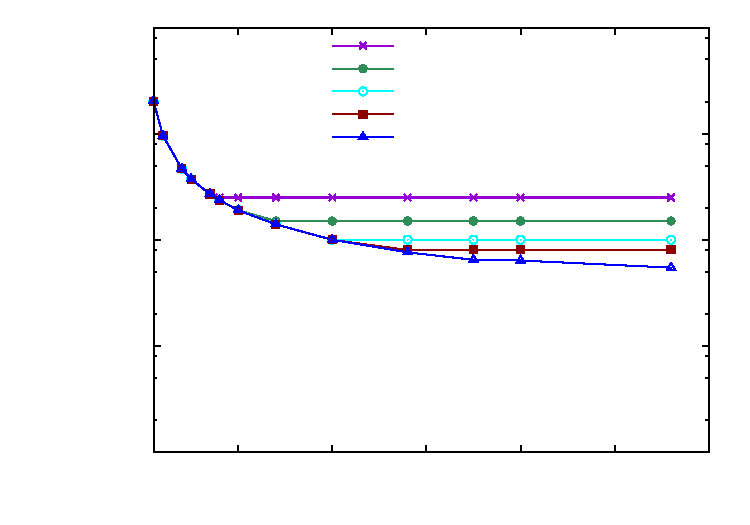
\includegraphics{plot-T_nogatherInt_00_500_selected_280}}%
    \gplfronttext
  \end{picture}%
\endgroup
}
      \caption{Tempo di servizio dell'implementazione UDN con M=280 al variare del tempo di interarrivo}
      \label{fig:scalability_UDN_size280}
    \end{subfigure}
    \label{fig:allScalbility_UDN}
  \end{subfigure}
  \hspace{2ex}
  \begin{subfigure}[b]{.5\columnwidth}
    \centering
    \renewcommand\thesubfigure{\alph{subfigure}}
    \caption{Implementazione con solo SM}
    \begin{subfigure}[b]{\textwidth}
      \centering
      \addtocounter{subfigure}{-1}
      \renewcommand\thesubfigure{\alph{subfigure}1}
      \resizebox{\columnwidth}{!}{% GNUPLOT: LaTeX picture with Postscript
\begingroup
  \makeatletter
  \providecommand\color[2][]{%
    \GenericError{(gnuplot) \space\space\space\@spaces}{%
      Package color not loaded in conjunction with
      terminal option `colourtext'%
    }{See the gnuplot documentation for explanation.%
    }{Either use 'blacktext' in gnuplot or load the package
      color.sty in LaTeX.}%
    \renewcommand\color[2][]{}%
  }%
  \providecommand\includegraphics[2][]{%
    \GenericError{(gnuplot) \space\space\space\@spaces}{%
      Package graphicx or graphics not loaded%
    }{See the gnuplot documentation for explanation.%
    }{The gnuplot epslatex terminal needs graphicx.sty or graphics.sty.}%
    \renewcommand\includegraphics[2][]{}%
  }%
  \providecommand\rotatebox[2]{#2}%
  \@ifundefined{ifGPcolor}{%
    \newif\ifGPcolor
    \GPcolortrue
  }{}%
  \@ifundefined{ifGPblacktext}{%
    \newif\ifGPblacktext
    \GPblacktexttrue
  }{}%
  % define a \g@addto@macro without @ in the name:
  \let\gplgaddtomacro\g@addto@macro
  % define empty templates for all commands taking text:
  \gdef\gplbacktext{}%
  \gdef\gplfronttext{}%
  \makeatother
  \ifGPblacktext
    % no textcolor at all
    \def\colorrgb#1{}%
    \def\colorgray#1{}%
  \else
    % gray or color?
    \ifGPcolor
      \def\colorrgb#1{\color[rgb]{#1}}%
      \def\colorgray#1{\color[gray]{#1}}%
      \expandafter\def\csname LTw\endcsname{\color{white}}%
      \expandafter\def\csname LTb\endcsname{\color{black}}%
      \expandafter\def\csname LTa\endcsname{\color{black}}%
      \expandafter\def\csname LT0\endcsname{\color[rgb]{1,0,0}}%
      \expandafter\def\csname LT1\endcsname{\color[rgb]{0,1,0}}%
      \expandafter\def\csname LT2\endcsname{\color[rgb]{0,0,1}}%
      \expandafter\def\csname LT3\endcsname{\color[rgb]{1,0,1}}%
      \expandafter\def\csname LT4\endcsname{\color[rgb]{0,1,1}}%
      \expandafter\def\csname LT5\endcsname{\color[rgb]{1,1,0}}%
      \expandafter\def\csname LT6\endcsname{\color[rgb]{0,0,0}}%
      \expandafter\def\csname LT7\endcsname{\color[rgb]{1,0.3,0}}%
      \expandafter\def\csname LT8\endcsname{\color[rgb]{0.5,0.5,0.5}}%
    \else
      % gray
      \def\colorrgb#1{\color{black}}%
      \def\colorgray#1{\color[gray]{#1}}%
      \expandafter\def\csname LTw\endcsname{\color{white}}%
      \expandafter\def\csname LTb\endcsname{\color{black}}%
      \expandafter\def\csname LTa\endcsname{\color{black}}%
      \expandafter\def\csname LT0\endcsname{\color{black}}%
      \expandafter\def\csname LT1\endcsname{\color{black}}%
      \expandafter\def\csname LT2\endcsname{\color{black}}%
      \expandafter\def\csname LT3\endcsname{\color{black}}%
      \expandafter\def\csname LT4\endcsname{\color{black}}%
      \expandafter\def\csname LT5\endcsname{\color{black}}%
      \expandafter\def\csname LT6\endcsname{\color{black}}%
      \expandafter\def\csname LT7\endcsname{\color{black}}%
      \expandafter\def\csname LT8\endcsname{\color{black}}%
    \fi
  \fi
  \setlength{\unitlength}{0.0500bp}%
  \begin{picture}(7200.00,5040.00)%
    \gplgaddtomacro\gplbacktext{%
      \csname LTb\endcsname%
      \put(1342,704){\makebox(0,0)[r]{\strut{} 1000}}%
      \put(1342,1722){\makebox(0,0)[r]{\strut{} 10000}}%
      \put(1342,2740){\makebox(0,0)[r]{\strut{} 100000}}%
      \put(1342,3757){\makebox(0,0)[r]{\strut{} 1e+06}}%
      \put(1342,4775){\makebox(0,0)[r]{\strut{} 1e+07}}%
      \put(2287,484){\makebox(0,0){\strut{} 10}}%
      \put(3190,484){\makebox(0,0){\strut{} 20}}%
      \put(4093,484){\makebox(0,0){\strut{} 30}}%
      \put(4997,484){\makebox(0,0){\strut{} 40}}%
      \put(5900,484){\makebox(0,0){\strut{} 50}}%
      \put(6803,484){\makebox(0,0){\strut{} 60}}%
      \put(176,2739){\rotatebox{-270}{\makebox(0,0){\strut{}service time ($\tau$)}}}%
      \put(4138,154){\makebox(0,0){\strut{}parallel degree}}%
    }%
    \gplgaddtomacro\gplfronttext{%
      \csname LTb\endcsname%
      \put(2926,4602){\makebox(0,0)[r]{\strut{}$T_A$ 20000 $\tau$}}%
      \csname LTb\endcsname%
      \put(2926,4382){\makebox(0,0)[r]{\strut{}$T_A$ 10000 $\tau$}}%
      \csname LTb\endcsname%
      \put(2926,4162){\makebox(0,0)[r]{\strut{}$T_A$ 7000 $\tau$}}%
      \csname LTb\endcsname%
      \put(2926,3942){\makebox(0,0)[r]{\strut{}$T_A$ 4000 $\tau$}}%
    }%
    \gplbacktext
    \put(0,0){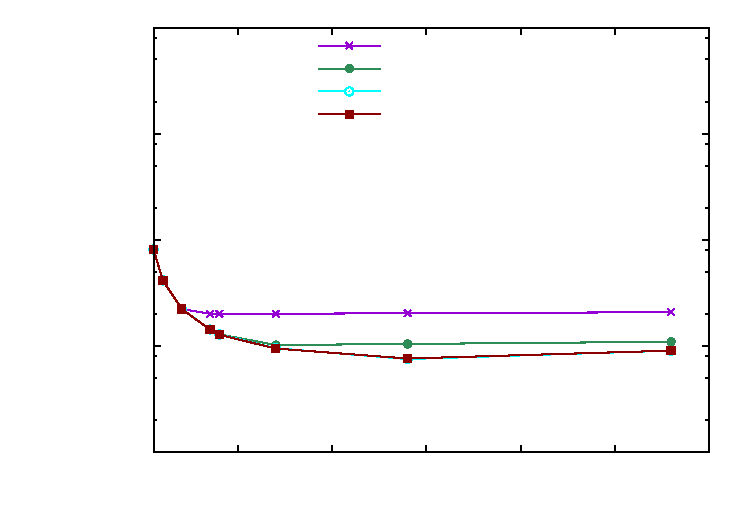
\includegraphics{plot-T_nogatherInt_11_500_selected_56}}%
    \gplfronttext
  \end{picture}%
\endgroup
}
      \caption{Tempo di servizio dell'implementazione SM con M=56 al variare del tempo di interarrivo}
      \label{fig:scalability_SM_size56}
    \end{subfigure}
    ~
    \begin{subfigure}[b]{\textwidth}
      \centering
      \addtocounter{subfigure}{-1}
      \renewcommand\thesubfigure{\alph{subfigure}2}
      \resizebox{\columnwidth}{!}{% GNUPLOT: LaTeX picture with Postscript
\begingroup
  \makeatletter
  \providecommand\color[2][]{%
    \GenericError{(gnuplot) \space\space\space\@spaces}{%
      Package color not loaded in conjunction with
      terminal option `colourtext'%
    }{See the gnuplot documentation for explanation.%
    }{Either use 'blacktext' in gnuplot or load the package
      color.sty in LaTeX.}%
    \renewcommand\color[2][]{}%
  }%
  \providecommand\includegraphics[2][]{%
    \GenericError{(gnuplot) \space\space\space\@spaces}{%
      Package graphicx or graphics not loaded%
    }{See the gnuplot documentation for explanation.%
    }{The gnuplot epslatex terminal needs graphicx.sty or graphics.sty.}%
    \renewcommand\includegraphics[2][]{}%
  }%
  \providecommand\rotatebox[2]{#2}%
  \@ifundefined{ifGPcolor}{%
    \newif\ifGPcolor
    \GPcolortrue
  }{}%
  \@ifundefined{ifGPblacktext}{%
    \newif\ifGPblacktext
    \GPblacktexttrue
  }{}%
  % define a \g@addto@macro without @ in the name:
  \let\gplgaddtomacro\g@addto@macro
  % define empty templates for all commands taking text:
  \gdef\gplbacktext{}%
  \gdef\gplfronttext{}%
  \makeatother
  \ifGPblacktext
    % no textcolor at all
    \def\colorrgb#1{}%
    \def\colorgray#1{}%
  \else
    % gray or color?
    \ifGPcolor
      \def\colorrgb#1{\color[rgb]{#1}}%
      \def\colorgray#1{\color[gray]{#1}}%
      \expandafter\def\csname LTw\endcsname{\color{white}}%
      \expandafter\def\csname LTb\endcsname{\color{black}}%
      \expandafter\def\csname LTa\endcsname{\color{black}}%
      \expandafter\def\csname LT0\endcsname{\color[rgb]{1,0,0}}%
      \expandafter\def\csname LT1\endcsname{\color[rgb]{0,1,0}}%
      \expandafter\def\csname LT2\endcsname{\color[rgb]{0,0,1}}%
      \expandafter\def\csname LT3\endcsname{\color[rgb]{1,0,1}}%
      \expandafter\def\csname LT4\endcsname{\color[rgb]{0,1,1}}%
      \expandafter\def\csname LT5\endcsname{\color[rgb]{1,1,0}}%
      \expandafter\def\csname LT6\endcsname{\color[rgb]{0,0,0}}%
      \expandafter\def\csname LT7\endcsname{\color[rgb]{1,0.3,0}}%
      \expandafter\def\csname LT8\endcsname{\color[rgb]{0.5,0.5,0.5}}%
    \else
      % gray
      \def\colorrgb#1{\color{black}}%
      \def\colorgray#1{\color[gray]{#1}}%
      \expandafter\def\csname LTw\endcsname{\color{white}}%
      \expandafter\def\csname LTb\endcsname{\color{black}}%
      \expandafter\def\csname LTa\endcsname{\color{black}}%
      \expandafter\def\csname LT0\endcsname{\color{black}}%
      \expandafter\def\csname LT1\endcsname{\color{black}}%
      \expandafter\def\csname LT2\endcsname{\color{black}}%
      \expandafter\def\csname LT3\endcsname{\color{black}}%
      \expandafter\def\csname LT4\endcsname{\color{black}}%
      \expandafter\def\csname LT5\endcsname{\color{black}}%
      \expandafter\def\csname LT6\endcsname{\color{black}}%
      \expandafter\def\csname LT7\endcsname{\color{black}}%
      \expandafter\def\csname LT8\endcsname{\color{black}}%
    \fi
  \fi
  \setlength{\unitlength}{0.0500bp}%
  \begin{picture}(7200.00,5040.00)%
    \gplgaddtomacro\gplbacktext{%
      \csname LTb\endcsname%
      \put(1342,704){\makebox(0,0)[r]{\strut{} 1000}}%
      \put(1342,1722){\makebox(0,0)[r]{\strut{} 10000}}%
      \put(1342,2740){\makebox(0,0)[r]{\strut{} 100000}}%
      \put(1342,3757){\makebox(0,0)[r]{\strut{} 1e+06}}%
      \put(1342,4775){\makebox(0,0)[r]{\strut{} 1e+07}}%
      \put(2287,484){\makebox(0,0){\strut{} 10}}%
      \put(3190,484){\makebox(0,0){\strut{} 20}}%
      \put(4093,484){\makebox(0,0){\strut{} 30}}%
      \put(4997,484){\makebox(0,0){\strut{} 40}}%
      \put(5900,484){\makebox(0,0){\strut{} 50}}%
      \put(6803,484){\makebox(0,0){\strut{} 60}}%
      \put(176,2739){\rotatebox{-270}{\makebox(0,0){\strut{}service time ($\tau$)}}}%
      \put(4138,154){\makebox(0,0){\strut{}parallel degree}}%
    }%
    \gplgaddtomacro\gplfronttext{%
      \csname LTb\endcsname%
      \put(3058,4602){\makebox(0,0)[r]{\strut{}$T_A$ 150000 $\tau$}}%
      \csname LTb\endcsname%
      \put(3058,4382){\makebox(0,0)[r]{\strut{}$T_A$ 80000 $\tau$}}%
      \csname LTb\endcsname%
      \put(3058,4162){\makebox(0,0)[r]{\strut{}$T_A$ 50000 $\tau$}}%
      \csname LTb\endcsname%
      \put(3058,3942){\makebox(0,0)[r]{\strut{}$T_A$ 35000 $\tau$}}%
      \csname LTb\endcsname%
      \put(3058,3722){\makebox(0,0)[r]{\strut{}$T_A$ 20000 $\tau$}}%
    }%
    \gplbacktext
    \put(0,0){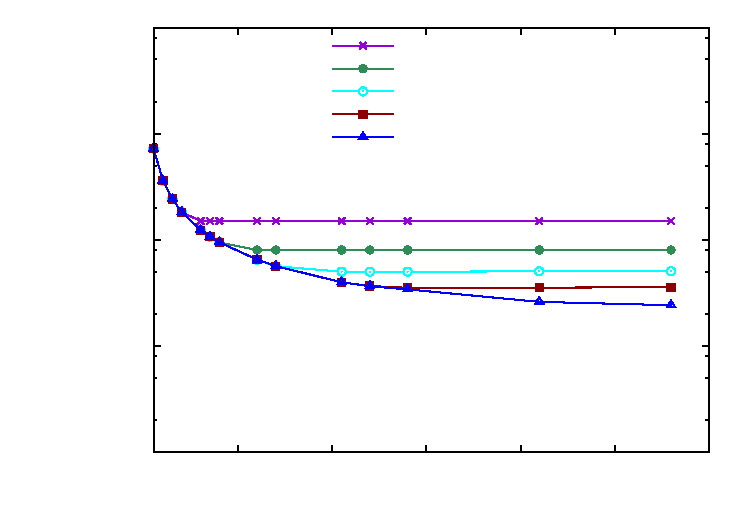
\includegraphics{plot-T_nogatherInt_11_500_selected_168}}%
    \gplfronttext
  \end{picture}%
\endgroup
}
      \caption{Tempo di servizio dell'implementazione SM con M=168 al variare del tempo di interarrivo}
      \label{fig:scalability_SM_size168}
    \end{subfigure}
    ~
    \begin{subfigure}[b]{\textwidth}
      \centering
      \addtocounter{subfigure}{-1}
      \renewcommand\thesubfigure{\alph{subfigure}3}
      \resizebox{\columnwidth}{!}{% GNUPLOT: LaTeX picture with Postscript
\begingroup
  \makeatletter
  \providecommand\color[2][]{%
    \GenericError{(gnuplot) \space\space\space\@spaces}{%
      Package color not loaded in conjunction with
      terminal option `colourtext'%
    }{See the gnuplot documentation for explanation.%
    }{Either use 'blacktext' in gnuplot or load the package
      color.sty in LaTeX.}%
    \renewcommand\color[2][]{}%
  }%
  \providecommand\includegraphics[2][]{%
    \GenericError{(gnuplot) \space\space\space\@spaces}{%
      Package graphicx or graphics not loaded%
    }{See the gnuplot documentation for explanation.%
    }{The gnuplot epslatex terminal needs graphicx.sty or graphics.sty.}%
    \renewcommand\includegraphics[2][]{}%
  }%
  \providecommand\rotatebox[2]{#2}%
  \@ifundefined{ifGPcolor}{%
    \newif\ifGPcolor
    \GPcolortrue
  }{}%
  \@ifundefined{ifGPblacktext}{%
    \newif\ifGPblacktext
    \GPblacktexttrue
  }{}%
  % define a \g@addto@macro without @ in the name:
  \let\gplgaddtomacro\g@addto@macro
  % define empty templates for all commands taking text:
  \gdef\gplbacktext{}%
  \gdef\gplfronttext{}%
  \makeatother
  \ifGPblacktext
    % no textcolor at all
    \def\colorrgb#1{}%
    \def\colorgray#1{}%
  \else
    % gray or color?
    \ifGPcolor
      \def\colorrgb#1{\color[rgb]{#1}}%
      \def\colorgray#1{\color[gray]{#1}}%
      \expandafter\def\csname LTw\endcsname{\color{white}}%
      \expandafter\def\csname LTb\endcsname{\color{black}}%
      \expandafter\def\csname LTa\endcsname{\color{black}}%
      \expandafter\def\csname LT0\endcsname{\color[rgb]{1,0,0}}%
      \expandafter\def\csname LT1\endcsname{\color[rgb]{0,1,0}}%
      \expandafter\def\csname LT2\endcsname{\color[rgb]{0,0,1}}%
      \expandafter\def\csname LT3\endcsname{\color[rgb]{1,0,1}}%
      \expandafter\def\csname LT4\endcsname{\color[rgb]{0,1,1}}%
      \expandafter\def\csname LT5\endcsname{\color[rgb]{1,1,0}}%
      \expandafter\def\csname LT6\endcsname{\color[rgb]{0,0,0}}%
      \expandafter\def\csname LT7\endcsname{\color[rgb]{1,0.3,0}}%
      \expandafter\def\csname LT8\endcsname{\color[rgb]{0.5,0.5,0.5}}%
    \else
      % gray
      \def\colorrgb#1{\color{black}}%
      \def\colorgray#1{\color[gray]{#1}}%
      \expandafter\def\csname LTw\endcsname{\color{white}}%
      \expandafter\def\csname LTb\endcsname{\color{black}}%
      \expandafter\def\csname LTa\endcsname{\color{black}}%
      \expandafter\def\csname LT0\endcsname{\color{black}}%
      \expandafter\def\csname LT1\endcsname{\color{black}}%
      \expandafter\def\csname LT2\endcsname{\color{black}}%
      \expandafter\def\csname LT3\endcsname{\color{black}}%
      \expandafter\def\csname LT4\endcsname{\color{black}}%
      \expandafter\def\csname LT5\endcsname{\color{black}}%
      \expandafter\def\csname LT6\endcsname{\color{black}}%
      \expandafter\def\csname LT7\endcsname{\color{black}}%
      \expandafter\def\csname LT8\endcsname{\color{black}}%
    \fi
  \fi
  \setlength{\unitlength}{0.0500bp}%
  \begin{picture}(7200.00,5040.00)%
    \gplgaddtomacro\gplbacktext{%
      \csname LTb\endcsname%
      \put(1342,704){\makebox(0,0)[r]{\strut{} 1000}}%
      \put(1342,1722){\makebox(0,0)[r]{\strut{} 10000}}%
      \put(1342,2740){\makebox(0,0)[r]{\strut{} 100000}}%
      \put(1342,3757){\makebox(0,0)[r]{\strut{} 1e+06}}%
      \put(1342,4775){\makebox(0,0)[r]{\strut{} 1e+07}}%
      \put(2287,484){\makebox(0,0){\strut{} 10}}%
      \put(3190,484){\makebox(0,0){\strut{} 20}}%
      \put(4093,484){\makebox(0,0){\strut{} 30}}%
      \put(4997,484){\makebox(0,0){\strut{} 40}}%
      \put(5900,484){\makebox(0,0){\strut{} 50}}%
      \put(6803,484){\makebox(0,0){\strut{} 60}}%
      \put(176,2739){\rotatebox{-270}{\makebox(0,0){\strut{}service time ($\tau$)}}}%
      \put(4138,154){\makebox(0,0){\strut{}parallel degree}}%
    }%
    \gplgaddtomacro\gplfronttext{%
      \csname LTb\endcsname%
      \put(3058,4602){\makebox(0,0)[r]{\strut{}$T_A$ 250000 $\tau$}}%
      \csname LTb\endcsname%
      \put(3058,4382){\makebox(0,0)[r]{\strut{}$T_A$ 150000 $\tau$}}%
      \csname LTb\endcsname%
      \put(3058,4162){\makebox(0,0)[r]{\strut{}$T_A$ 100000 $\tau$}}%
      \csname LTb\endcsname%
      \put(3058,3942){\makebox(0,0)[r]{\strut{}$T_A$ 80000 $\tau$}}%
      \csname LTb\endcsname%
      \put(3058,3722){\makebox(0,0)[r]{\strut{}$T_A$ 50000 $\tau$}}%
    }%
    \gplbacktext
    \put(0,0){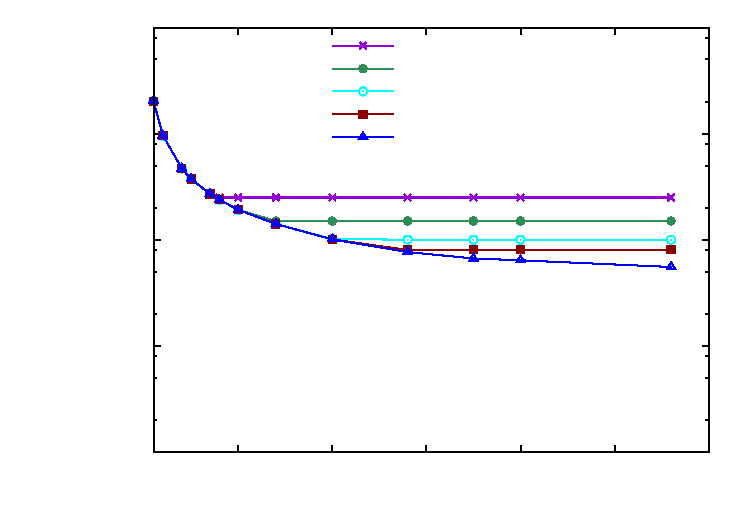
\includegraphics{plot-T_nogatherInt_11_500_selected_280}}%
    \gplfronttext
  \end{picture}%
\endgroup
}
      \caption{Tempo di servizio dell'implementazione SM con M=280 al variare del tempo di interarrivo}
      \label{fig:scalability_SM_size280}
    \end{subfigure}
    \label{fig:allscalability_SM}
  \end{subfigure}
\end{figure}


%%%%%%%%%%%%%%%%%%%%%%%%%%%%%%%%%%%%%%%%%%%%%%%%%%%%%%%%%%%%%%%%%%%%%%%%%%%%%%%%




%%%%%%%%%%%%%%%%%%%%%%%%%%%%%%%%%%%%%%%%%%%%%%%%%%%%%%%%%%%%%%%%%%%%%%%%%%%%%%%%

\newpage
%% \FloatBarrier
%% \subsection{Multicast service time}

%% \begin{lstlisting}[morekeywords={multicast_start, multicast_sum}]
%% void * generator_task(void *args...) {
%%   ...
%%   pthread_barrier_wait(...);
%%   for (i=0; i<m; i++) {
%%     a = get_clock_cycle();
%%     sym_send(ch_out, A_set[i]);
%%     while (get_clock_cycle() - a < Ta) 
%%       ;
%%   }
%%   ...
%% }

%% void * worker_task(void *args...) {
%%   ...
%%   pthread_barrier_wait(...);
%%   for (i=0; i<m; i++) {
%%     A = (int *)sym_receive(ch_in);
%%     atomic_compiler_barrier();
%%     if (rank == 0)
%%       multicast_start = get_clock_cycle();
%%     atomic_compiler_barrier();
%%     if (ch_left != NULL) sym_send(ch_left, A);
%%     if (ch_right != NULL) sym_send(ch_right, A);
%%     atomic_compiler_barrier();
%%     if (rank == 0)
%%       multicast_sum = get_clock_cycle() - multicast_start;
%%     atomic_compiler_barrier();
%%     for (j=0; j<g; j++) {
%%       C[j*rank] = 0;
%%       for (k=0; k<M; k++) 
%%         C[j*rank] = *(A+j*M+k) * B[k] + C[j*rank];
%%     }
%%     asymin_send(ch_out, C);
%%   }
%%   if (rank == 0)
%%     fprintf(output_file, ``%d %f\n'', n, (double)multicast_sum/m);
%%   ...
%% }

%% void * collector_task(void *args...) {
%%   ...
%%   pthread_barrier_wait(...);
%%   for (i=0; i<m; i++) {
%%     (void)asymin_receive(ch_in);
%%   }
%%   ...
%% }
%% \end{lstlisting}

\begin{figure}[p]
  \caption{Grafici del tempo di multicast al variare del tempo di interarrivo}
  \begin{subfigure}[b]{.5\columnwidth}
    \centering
    \renewcommand\thesubfigure{\alph{subfigure}}
    %% se vuoi spostare questa caption in fondo devi modificare anche i contatori!
    \caption{Implementazione con solo UDN}
    \begin{subfigure}[b]{\textwidth}
      \centering
      \addtocounter{subfigure}{-1}
      \renewcommand\thesubfigure{\alph{subfigure}1}
      \resizebox{\columnwidth}{!}{% GNUPLOT: LaTeX picture with Postscript
\begingroup
  \makeatletter
  \providecommand\color[2][]{%
    \GenericError{(gnuplot) \space\space\space\@spaces}{%
      Package color not loaded in conjunction with
      terminal option `colourtext'%
    }{See the gnuplot documentation for explanation.%
    }{Either use 'blacktext' in gnuplot or load the package
      color.sty in LaTeX.}%
    \renewcommand\color[2][]{}%
  }%
  \providecommand\includegraphics[2][]{%
    \GenericError{(gnuplot) \space\space\space\@spaces}{%
      Package graphicx or graphics not loaded%
    }{See the gnuplot documentation for explanation.%
    }{The gnuplot epslatex terminal needs graphicx.sty or graphics.sty.}%
    \renewcommand\includegraphics[2][]{}%
  }%
  \providecommand\rotatebox[2]{#2}%
  \@ifundefined{ifGPcolor}{%
    \newif\ifGPcolor
    \GPcolortrue
  }{}%
  \@ifundefined{ifGPblacktext}{%
    \newif\ifGPblacktext
    \GPblacktexttrue
  }{}%
  % define a \g@addto@macro without @ in the name:
  \let\gplgaddtomacro\g@addto@macro
  % define empty templates for all commands taking text:
  \gdef\gplbacktext{}%
  \gdef\gplfronttext{}%
  \makeatother
  \ifGPblacktext
    % no textcolor at all
    \def\colorrgb#1{}%
    \def\colorgray#1{}%
  \else
    % gray or color?
    \ifGPcolor
      \def\colorrgb#1{\color[rgb]{#1}}%
      \def\colorgray#1{\color[gray]{#1}}%
      \expandafter\def\csname LTw\endcsname{\color{white}}%
      \expandafter\def\csname LTb\endcsname{\color{black}}%
      \expandafter\def\csname LTa\endcsname{\color{black}}%
      \expandafter\def\csname LT0\endcsname{\color[rgb]{1,0,0}}%
      \expandafter\def\csname LT1\endcsname{\color[rgb]{0,1,0}}%
      \expandafter\def\csname LT2\endcsname{\color[rgb]{0,0,1}}%
      \expandafter\def\csname LT3\endcsname{\color[rgb]{1,0,1}}%
      \expandafter\def\csname LT4\endcsname{\color[rgb]{0,1,1}}%
      \expandafter\def\csname LT5\endcsname{\color[rgb]{1,1,0}}%
      \expandafter\def\csname LT6\endcsname{\color[rgb]{0,0,0}}%
      \expandafter\def\csname LT7\endcsname{\color[rgb]{1,0.3,0}}%
      \expandafter\def\csname LT8\endcsname{\color[rgb]{0.5,0.5,0.5}}%
    \else
      % gray
      \def\colorrgb#1{\color{black}}%
      \def\colorgray#1{\color[gray]{#1}}%
      \expandafter\def\csname LTw\endcsname{\color{white}}%
      \expandafter\def\csname LTb\endcsname{\color{black}}%
      \expandafter\def\csname LTa\endcsname{\color{black}}%
      \expandafter\def\csname LT0\endcsname{\color{black}}%
      \expandafter\def\csname LT1\endcsname{\color{black}}%
      \expandafter\def\csname LT2\endcsname{\color{black}}%
      \expandafter\def\csname LT3\endcsname{\color{black}}%
      \expandafter\def\csname LT4\endcsname{\color{black}}%
      \expandafter\def\csname LT5\endcsname{\color{black}}%
      \expandafter\def\csname LT6\endcsname{\color{black}}%
      \expandafter\def\csname LT7\endcsname{\color{black}}%
      \expandafter\def\csname LT8\endcsname{\color{black}}%
    \fi
  \fi
  \setlength{\unitlength}{0.0500bp}%
  \begin{picture}(7200.00,5040.00)%
    \gplgaddtomacro\gplbacktext{%
      \csname LTb\endcsname%
      \put(1078,704){\makebox(0,0)[r]{\strut{} 0}}%
      \put(1078,1673){\makebox(0,0)[r]{\strut{} 500}}%
      \put(1078,2643){\makebox(0,0)[r]{\strut{} 1000}}%
      \put(1078,3612){\makebox(0,0)[r]{\strut{} 1500}}%
      \put(1078,4581){\makebox(0,0)[r]{\strut{} 2000}}%
      \put(2063,484){\makebox(0,0){\strut{} 10}}%
      \put(3011,484){\makebox(0,0){\strut{} 20}}%
      \put(3959,484){\makebox(0,0){\strut{} 30}}%
      \put(4907,484){\makebox(0,0){\strut{} 40}}%
      \put(5855,484){\makebox(0,0){\strut{} 50}}%
      \put(6803,484){\makebox(0,0){\strut{} 60}}%
      \put(176,2739){\rotatebox{-270}{\makebox(0,0){\strut{}multicast service time}}}%
      \put(4006,154){\makebox(0,0){\strut{}$n$parallel degree}}%
    }%
    \gplgaddtomacro\gplfronttext{%
      \csname LTb\endcsname%
      \put(2662,4602){\makebox(0,0)[r]{\strut{}$T_A$ 20000 $\tau$}}%
      \csname LTb\endcsname%
      \put(2662,4382){\makebox(0,0)[r]{\strut{}$T_A$ 10000 $\tau$}}%
      \csname LTb\endcsname%
      \put(2662,4162){\makebox(0,0)[r]{\strut{}$T_A$ 7000 $\tau$}}%
    }%
    \gplbacktext
    \put(0,0){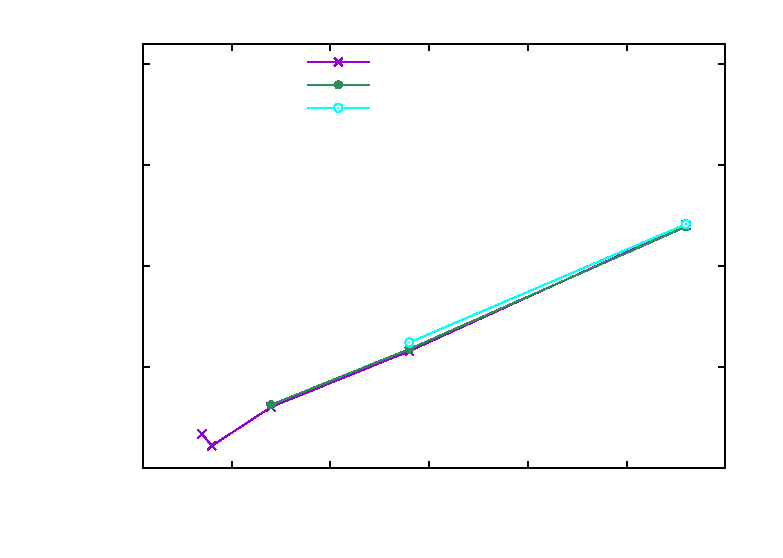
\includegraphics{plot-Tmult-nb_nogatherInt_00_500_selected_56}}%
    \gplfronttext
  \end{picture}%
\endgroup
}
      \caption{tempo di multicast dell implementazione UDN con M=56 al variare del tempo di interarrivo}
      \label{fig:scalability_UDN_size56}
    \end{subfigure}
    ~
    \begin{subfigure}[b]{\textwidth}
      \centering
      \addtocounter{subfigure}{-1}
      \renewcommand\thesubfigure{\alph{subfigure}2}
      \resizebox{\columnwidth}{!}{% GNUPLOT: LaTeX picture with Postscript
\begingroup
  \makeatletter
  \providecommand\color[2][]{%
    \GenericError{(gnuplot) \space\space\space\@spaces}{%
      Package color not loaded in conjunction with
      terminal option `colourtext'%
    }{See the gnuplot documentation for explanation.%
    }{Either use 'blacktext' in gnuplot or load the package
      color.sty in LaTeX.}%
    \renewcommand\color[2][]{}%
  }%
  \providecommand\includegraphics[2][]{%
    \GenericError{(gnuplot) \space\space\space\@spaces}{%
      Package graphicx or graphics not loaded%
    }{See the gnuplot documentation for explanation.%
    }{The gnuplot epslatex terminal needs graphicx.sty or graphics.sty.}%
    \renewcommand\includegraphics[2][]{}%
  }%
  \providecommand\rotatebox[2]{#2}%
  \@ifundefined{ifGPcolor}{%
    \newif\ifGPcolor
    \GPcolortrue
  }{}%
  \@ifundefined{ifGPblacktext}{%
    \newif\ifGPblacktext
    \GPblacktexttrue
  }{}%
  % define a \g@addto@macro without @ in the name:
  \let\gplgaddtomacro\g@addto@macro
  % define empty templates for all commands taking text:
  \gdef\gplbacktext{}%
  \gdef\gplfronttext{}%
  \makeatother
  \ifGPblacktext
    % no textcolor at all
    \def\colorrgb#1{}%
    \def\colorgray#1{}%
  \else
    % gray or color?
    \ifGPcolor
      \def\colorrgb#1{\color[rgb]{#1}}%
      \def\colorgray#1{\color[gray]{#1}}%
      \expandafter\def\csname LTw\endcsname{\color{white}}%
      \expandafter\def\csname LTb\endcsname{\color{black}}%
      \expandafter\def\csname LTa\endcsname{\color{black}}%
      \expandafter\def\csname LT0\endcsname{\color[rgb]{1,0,0}}%
      \expandafter\def\csname LT1\endcsname{\color[rgb]{0,1,0}}%
      \expandafter\def\csname LT2\endcsname{\color[rgb]{0,0,1}}%
      \expandafter\def\csname LT3\endcsname{\color[rgb]{1,0,1}}%
      \expandafter\def\csname LT4\endcsname{\color[rgb]{0,1,1}}%
      \expandafter\def\csname LT5\endcsname{\color[rgb]{1,1,0}}%
      \expandafter\def\csname LT6\endcsname{\color[rgb]{0,0,0}}%
      \expandafter\def\csname LT7\endcsname{\color[rgb]{1,0.3,0}}%
      \expandafter\def\csname LT8\endcsname{\color[rgb]{0.5,0.5,0.5}}%
    \else
      % gray
      \def\colorrgb#1{\color{black}}%
      \def\colorgray#1{\color[gray]{#1}}%
      \expandafter\def\csname LTw\endcsname{\color{white}}%
      \expandafter\def\csname LTb\endcsname{\color{black}}%
      \expandafter\def\csname LTa\endcsname{\color{black}}%
      \expandafter\def\csname LT0\endcsname{\color{black}}%
      \expandafter\def\csname LT1\endcsname{\color{black}}%
      \expandafter\def\csname LT2\endcsname{\color{black}}%
      \expandafter\def\csname LT3\endcsname{\color{black}}%
      \expandafter\def\csname LT4\endcsname{\color{black}}%
      \expandafter\def\csname LT5\endcsname{\color{black}}%
      \expandafter\def\csname LT6\endcsname{\color{black}}%
      \expandafter\def\csname LT7\endcsname{\color{black}}%
      \expandafter\def\csname LT8\endcsname{\color{black}}%
    \fi
  \fi
  \setlength{\unitlength}{0.0500bp}%
  \begin{picture}(7200.00,5040.00)%
    \gplgaddtomacro\gplbacktext{%
      \csname LTb\endcsname%
      \put(1078,704){\makebox(0,0)[r]{\strut{} 0}}%
      \put(1078,1673){\makebox(0,0)[r]{\strut{} 500}}%
      \put(1078,2643){\makebox(0,0)[r]{\strut{} 1000}}%
      \put(1078,3612){\makebox(0,0)[r]{\strut{} 1500}}%
      \put(1078,4581){\makebox(0,0)[r]{\strut{} 2000}}%
      \put(2063,484){\makebox(0,0){\strut{} 10}}%
      \put(3011,484){\makebox(0,0){\strut{} 20}}%
      \put(3959,484){\makebox(0,0){\strut{} 30}}%
      \put(4907,484){\makebox(0,0){\strut{} 40}}%
      \put(5855,484){\makebox(0,0){\strut{} 50}}%
      \put(6803,484){\makebox(0,0){\strut{} 60}}%
      \put(176,2739){\rotatebox{-270}{\makebox(0,0){\strut{}multicast service time}}}%
      \put(4006,154){\makebox(0,0){\strut{}$n$parallel degree}}%
    }%
    \gplgaddtomacro\gplfronttext{%
      \csname LTb\endcsname%
      \put(2794,4602){\makebox(0,0)[r]{\strut{}$T_A$ 150000 $\tau$}}%
      \csname LTb\endcsname%
      \put(2794,4382){\makebox(0,0)[r]{\strut{}$T_A$ 80000 $\tau$}}%
      \csname LTb\endcsname%
      \put(2794,4162){\makebox(0,0)[r]{\strut{}$T_A$ 50000 $\tau$}}%
      \csname LTb\endcsname%
      \put(2794,3942){\makebox(0,0)[r]{\strut{}$T_A$ 35000 $\tau$}}%
    }%
    \gplbacktext
    \put(0,0){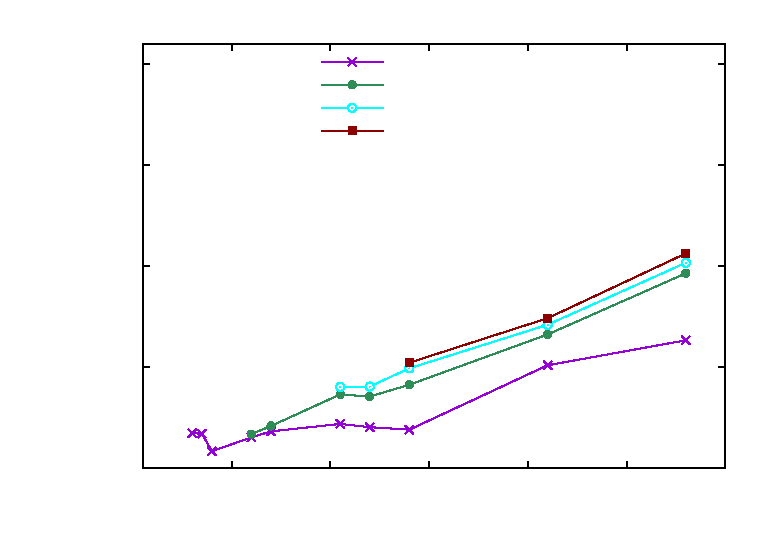
\includegraphics{plot-Tmult-nb_nogatherInt_00_500_selected_168}}%
    \gplfronttext
  \end{picture}%
\endgroup
}
      \caption{tempo di multicast dell implementazione UDN con M=168 al variare del tempo di interarrivo}
      \label{fig:scalability_UDN_size168}
    \end{subfigure}
    ~
    \begin{subfigure}[b]{\textwidth}
      \centering
      \addtocounter{subfigure}{-1}
      \renewcommand\thesubfigure{\alph{subfigure}3}
      \resizebox{\columnwidth}{!}{% GNUPLOT: LaTeX picture with Postscript
\begingroup
  \makeatletter
  \providecommand\color[2][]{%
    \GenericError{(gnuplot) \space\space\space\@spaces}{%
      Package color not loaded in conjunction with
      terminal option `colourtext'%
    }{See the gnuplot documentation for explanation.%
    }{Either use 'blacktext' in gnuplot or load the package
      color.sty in LaTeX.}%
    \renewcommand\color[2][]{}%
  }%
  \providecommand\includegraphics[2][]{%
    \GenericError{(gnuplot) \space\space\space\@spaces}{%
      Package graphicx or graphics not loaded%
    }{See the gnuplot documentation for explanation.%
    }{The gnuplot epslatex terminal needs graphicx.sty or graphics.sty.}%
    \renewcommand\includegraphics[2][]{}%
  }%
  \providecommand\rotatebox[2]{#2}%
  \@ifundefined{ifGPcolor}{%
    \newif\ifGPcolor
    \GPcolortrue
  }{}%
  \@ifundefined{ifGPblacktext}{%
    \newif\ifGPblacktext
    \GPblacktexttrue
  }{}%
  % define a \g@addto@macro without @ in the name:
  \let\gplgaddtomacro\g@addto@macro
  % define empty templates for all commands taking text:
  \gdef\gplbacktext{}%
  \gdef\gplfronttext{}%
  \makeatother
  \ifGPblacktext
    % no textcolor at all
    \def\colorrgb#1{}%
    \def\colorgray#1{}%
  \else
    % gray or color?
    \ifGPcolor
      \def\colorrgb#1{\color[rgb]{#1}}%
      \def\colorgray#1{\color[gray]{#1}}%
      \expandafter\def\csname LTw\endcsname{\color{white}}%
      \expandafter\def\csname LTb\endcsname{\color{black}}%
      \expandafter\def\csname LTa\endcsname{\color{black}}%
      \expandafter\def\csname LT0\endcsname{\color[rgb]{1,0,0}}%
      \expandafter\def\csname LT1\endcsname{\color[rgb]{0,1,0}}%
      \expandafter\def\csname LT2\endcsname{\color[rgb]{0,0,1}}%
      \expandafter\def\csname LT3\endcsname{\color[rgb]{1,0,1}}%
      \expandafter\def\csname LT4\endcsname{\color[rgb]{0,1,1}}%
      \expandafter\def\csname LT5\endcsname{\color[rgb]{1,1,0}}%
      \expandafter\def\csname LT6\endcsname{\color[rgb]{0,0,0}}%
      \expandafter\def\csname LT7\endcsname{\color[rgb]{1,0.3,0}}%
      \expandafter\def\csname LT8\endcsname{\color[rgb]{0.5,0.5,0.5}}%
    \else
      % gray
      \def\colorrgb#1{\color{black}}%
      \def\colorgray#1{\color[gray]{#1}}%
      \expandafter\def\csname LTw\endcsname{\color{white}}%
      \expandafter\def\csname LTb\endcsname{\color{black}}%
      \expandafter\def\csname LTa\endcsname{\color{black}}%
      \expandafter\def\csname LT0\endcsname{\color{black}}%
      \expandafter\def\csname LT1\endcsname{\color{black}}%
      \expandafter\def\csname LT2\endcsname{\color{black}}%
      \expandafter\def\csname LT3\endcsname{\color{black}}%
      \expandafter\def\csname LT4\endcsname{\color{black}}%
      \expandafter\def\csname LT5\endcsname{\color{black}}%
      \expandafter\def\csname LT6\endcsname{\color{black}}%
      \expandafter\def\csname LT7\endcsname{\color{black}}%
      \expandafter\def\csname LT8\endcsname{\color{black}}%
    \fi
  \fi
  \setlength{\unitlength}{0.0500bp}%
  \begin{picture}(7200.00,5040.00)%
    \gplgaddtomacro\gplbacktext{%
      \csname LTb\endcsname%
      \put(1078,704){\makebox(0,0)[r]{\strut{} 0}}%
      \put(1078,1673){\makebox(0,0)[r]{\strut{} 500}}%
      \put(1078,2643){\makebox(0,0)[r]{\strut{} 1000}}%
      \put(1078,3612){\makebox(0,0)[r]{\strut{} 1500}}%
      \put(1078,4581){\makebox(0,0)[r]{\strut{} 2000}}%
      \put(2063,484){\makebox(0,0){\strut{} 10}}%
      \put(3011,484){\makebox(0,0){\strut{} 20}}%
      \put(3959,484){\makebox(0,0){\strut{} 30}}%
      \put(4907,484){\makebox(0,0){\strut{} 40}}%
      \put(5855,484){\makebox(0,0){\strut{} 50}}%
      \put(6803,484){\makebox(0,0){\strut{} 60}}%
      \put(176,2739){\rotatebox{-270}{\makebox(0,0){\strut{}multicast service time}}}%
      \put(4006,154){\makebox(0,0){\strut{}$n$parallel degree}}%
    }%
    \gplgaddtomacro\gplfronttext{%
      \csname LTb\endcsname%
      \put(2794,4602){\makebox(0,0)[r]{\strut{}$T_A$ 250000 $\tau$}}%
      \csname LTb\endcsname%
      \put(2794,4382){\makebox(0,0)[r]{\strut{}$T_A$ 150000 $\tau$}}%
      \csname LTb\endcsname%
      \put(2794,4162){\makebox(0,0)[r]{\strut{}$T_A$ 100000 $\tau$}}%
      \csname LTb\endcsname%
      \put(2794,3942){\makebox(0,0)[r]{\strut{}$T_A$ 80000 $\tau$}}%
    }%
    \gplbacktext
    \put(0,0){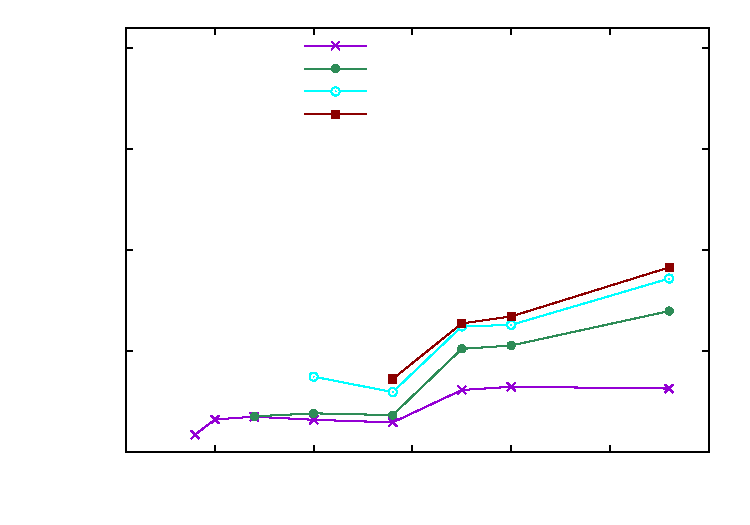
\includegraphics{plot-Tmult-nb_nogatherInt_00_500_selected_280}}%
    \gplfronttext
  \end{picture}%
\endgroup
}
      \caption{tempo di multicast dell implementazione UDN con M=280 al variare del tempo di interarrivo}
      \label{fig:scalability_UDN_size280}
    \end{subfigure}
    \label{fig:allScalbility_UDN}
  \end{subfigure}
  \hspace{2ex}
  \begin{subfigure}[b]{.5\columnwidth}
    \centering
    \renewcommand\thesubfigure{\alph{subfigure}}
    \caption{Implementazione con solo SM}
    \begin{subfigure}[b]{\textwidth}
      \centering
      \addtocounter{subfigure}{-1}
      \renewcommand\thesubfigure{\alph{subfigure}1}
      \resizebox{\columnwidth}{!}{% GNUPLOT: LaTeX picture with Postscript
\begingroup
  \makeatletter
  \providecommand\color[2][]{%
    \GenericError{(gnuplot) \space\space\space\@spaces}{%
      Package color not loaded in conjunction with
      terminal option `colourtext'%
    }{See the gnuplot documentation for explanation.%
    }{Either use 'blacktext' in gnuplot or load the package
      color.sty in LaTeX.}%
    \renewcommand\color[2][]{}%
  }%
  \providecommand\includegraphics[2][]{%
    \GenericError{(gnuplot) \space\space\space\@spaces}{%
      Package graphicx or graphics not loaded%
    }{See the gnuplot documentation for explanation.%
    }{The gnuplot epslatex terminal needs graphicx.sty or graphics.sty.}%
    \renewcommand\includegraphics[2][]{}%
  }%
  \providecommand\rotatebox[2]{#2}%
  \@ifundefined{ifGPcolor}{%
    \newif\ifGPcolor
    \GPcolortrue
  }{}%
  \@ifundefined{ifGPblacktext}{%
    \newif\ifGPblacktext
    \GPblacktexttrue
  }{}%
  % define a \g@addto@macro without @ in the name:
  \let\gplgaddtomacro\g@addto@macro
  % define empty templates for all commands taking text:
  \gdef\gplbacktext{}%
  \gdef\gplfronttext{}%
  \makeatother
  \ifGPblacktext
    % no textcolor at all
    \def\colorrgb#1{}%
    \def\colorgray#1{}%
  \else
    % gray or color?
    \ifGPcolor
      \def\colorrgb#1{\color[rgb]{#1}}%
      \def\colorgray#1{\color[gray]{#1}}%
      \expandafter\def\csname LTw\endcsname{\color{white}}%
      \expandafter\def\csname LTb\endcsname{\color{black}}%
      \expandafter\def\csname LTa\endcsname{\color{black}}%
      \expandafter\def\csname LT0\endcsname{\color[rgb]{1,0,0}}%
      \expandafter\def\csname LT1\endcsname{\color[rgb]{0,1,0}}%
      \expandafter\def\csname LT2\endcsname{\color[rgb]{0,0,1}}%
      \expandafter\def\csname LT3\endcsname{\color[rgb]{1,0,1}}%
      \expandafter\def\csname LT4\endcsname{\color[rgb]{0,1,1}}%
      \expandafter\def\csname LT5\endcsname{\color[rgb]{1,1,0}}%
      \expandafter\def\csname LT6\endcsname{\color[rgb]{0,0,0}}%
      \expandafter\def\csname LT7\endcsname{\color[rgb]{1,0.3,0}}%
      \expandafter\def\csname LT8\endcsname{\color[rgb]{0.5,0.5,0.5}}%
    \else
      % gray
      \def\colorrgb#1{\color{black}}%
      \def\colorgray#1{\color[gray]{#1}}%
      \expandafter\def\csname LTw\endcsname{\color{white}}%
      \expandafter\def\csname LTb\endcsname{\color{black}}%
      \expandafter\def\csname LTa\endcsname{\color{black}}%
      \expandafter\def\csname LT0\endcsname{\color{black}}%
      \expandafter\def\csname LT1\endcsname{\color{black}}%
      \expandafter\def\csname LT2\endcsname{\color{black}}%
      \expandafter\def\csname LT3\endcsname{\color{black}}%
      \expandafter\def\csname LT4\endcsname{\color{black}}%
      \expandafter\def\csname LT5\endcsname{\color{black}}%
      \expandafter\def\csname LT6\endcsname{\color{black}}%
      \expandafter\def\csname LT7\endcsname{\color{black}}%
      \expandafter\def\csname LT8\endcsname{\color{black}}%
    \fi
  \fi
  \setlength{\unitlength}{0.0500bp}%
  \begin{picture}(7200.00,5040.00)%
    \gplgaddtomacro\gplbacktext{%
      \csname LTb\endcsname%
      \put(1078,704){\makebox(0,0)[r]{\strut{} 0}}%
      \put(1078,1673){\makebox(0,0)[r]{\strut{} 500}}%
      \put(1078,2643){\makebox(0,0)[r]{\strut{} 1000}}%
      \put(1078,3612){\makebox(0,0)[r]{\strut{} 1500}}%
      \put(1078,4581){\makebox(0,0)[r]{\strut{} 2000}}%
      \put(2063,484){\makebox(0,0){\strut{} 10}}%
      \put(3011,484){\makebox(0,0){\strut{} 20}}%
      \put(3959,484){\makebox(0,0){\strut{} 30}}%
      \put(4907,484){\makebox(0,0){\strut{} 40}}%
      \put(5855,484){\makebox(0,0){\strut{} 50}}%
      \put(6803,484){\makebox(0,0){\strut{} 60}}%
      \put(176,2739){\rotatebox{-270}{\makebox(0,0){\strut{}multicast service time}}}%
      \put(4006,154){\makebox(0,0){\strut{}$n$parallel degree}}%
    }%
    \gplgaddtomacro\gplfronttext{%
      \csname LTb\endcsname%
      \put(2662,4602){\makebox(0,0)[r]{\strut{}$T_A$ 20000 $\tau$}}%
      \csname LTb\endcsname%
      \put(2662,4382){\makebox(0,0)[r]{\strut{}$T_A$ 10000 $\tau$}}%
    }%
    \gplbacktext
    \put(0,0){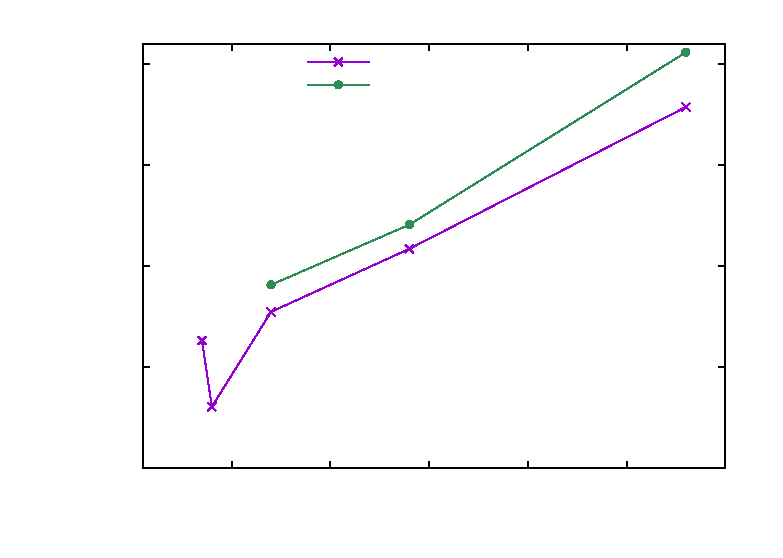
\includegraphics{plot-Tmult-nb_nogatherInt_11_500_selected_56}}%
    \gplfronttext
  \end{picture}%
\endgroup
}
      \caption{tempo di multicast dell implementazione SM con M=56 al variare del tempo di interarrivo}
      \label{fig:scalability_SM_size56}
    \end{subfigure}
    ~
    \begin{subfigure}[b]{\textwidth}
      \centering
      \addtocounter{subfigure}{-1}
      \renewcommand\thesubfigure{\alph{subfigure}2}
      \resizebox{\columnwidth}{!}{% GNUPLOT: LaTeX picture with Postscript
\begingroup
  \makeatletter
  \providecommand\color[2][]{%
    \GenericError{(gnuplot) \space\space\space\@spaces}{%
      Package color not loaded in conjunction with
      terminal option `colourtext'%
    }{See the gnuplot documentation for explanation.%
    }{Either use 'blacktext' in gnuplot or load the package
      color.sty in LaTeX.}%
    \renewcommand\color[2][]{}%
  }%
  \providecommand\includegraphics[2][]{%
    \GenericError{(gnuplot) \space\space\space\@spaces}{%
      Package graphicx or graphics not loaded%
    }{See the gnuplot documentation for explanation.%
    }{The gnuplot epslatex terminal needs graphicx.sty or graphics.sty.}%
    \renewcommand\includegraphics[2][]{}%
  }%
  \providecommand\rotatebox[2]{#2}%
  \@ifundefined{ifGPcolor}{%
    \newif\ifGPcolor
    \GPcolortrue
  }{}%
  \@ifundefined{ifGPblacktext}{%
    \newif\ifGPblacktext
    \GPblacktexttrue
  }{}%
  % define a \g@addto@macro without @ in the name:
  \let\gplgaddtomacro\g@addto@macro
  % define empty templates for all commands taking text:
  \gdef\gplbacktext{}%
  \gdef\gplfronttext{}%
  \makeatother
  \ifGPblacktext
    % no textcolor at all
    \def\colorrgb#1{}%
    \def\colorgray#1{}%
  \else
    % gray or color?
    \ifGPcolor
      \def\colorrgb#1{\color[rgb]{#1}}%
      \def\colorgray#1{\color[gray]{#1}}%
      \expandafter\def\csname LTw\endcsname{\color{white}}%
      \expandafter\def\csname LTb\endcsname{\color{black}}%
      \expandafter\def\csname LTa\endcsname{\color{black}}%
      \expandafter\def\csname LT0\endcsname{\color[rgb]{1,0,0}}%
      \expandafter\def\csname LT1\endcsname{\color[rgb]{0,1,0}}%
      \expandafter\def\csname LT2\endcsname{\color[rgb]{0,0,1}}%
      \expandafter\def\csname LT3\endcsname{\color[rgb]{1,0,1}}%
      \expandafter\def\csname LT4\endcsname{\color[rgb]{0,1,1}}%
      \expandafter\def\csname LT5\endcsname{\color[rgb]{1,1,0}}%
      \expandafter\def\csname LT6\endcsname{\color[rgb]{0,0,0}}%
      \expandafter\def\csname LT7\endcsname{\color[rgb]{1,0.3,0}}%
      \expandafter\def\csname LT8\endcsname{\color[rgb]{0.5,0.5,0.5}}%
    \else
      % gray
      \def\colorrgb#1{\color{black}}%
      \def\colorgray#1{\color[gray]{#1}}%
      \expandafter\def\csname LTw\endcsname{\color{white}}%
      \expandafter\def\csname LTb\endcsname{\color{black}}%
      \expandafter\def\csname LTa\endcsname{\color{black}}%
      \expandafter\def\csname LT0\endcsname{\color{black}}%
      \expandafter\def\csname LT1\endcsname{\color{black}}%
      \expandafter\def\csname LT2\endcsname{\color{black}}%
      \expandafter\def\csname LT3\endcsname{\color{black}}%
      \expandafter\def\csname LT4\endcsname{\color{black}}%
      \expandafter\def\csname LT5\endcsname{\color{black}}%
      \expandafter\def\csname LT6\endcsname{\color{black}}%
      \expandafter\def\csname LT7\endcsname{\color{black}}%
      \expandafter\def\csname LT8\endcsname{\color{black}}%
    \fi
  \fi
  \setlength{\unitlength}{0.0500bp}%
  \begin{picture}(7200.00,5040.00)%
    \gplgaddtomacro\gplbacktext{%
      \csname LTb\endcsname%
      \put(1078,704){\makebox(0,0)[r]{\strut{} 0}}%
      \put(1078,1673){\makebox(0,0)[r]{\strut{} 500}}%
      \put(1078,2643){\makebox(0,0)[r]{\strut{} 1000}}%
      \put(1078,3612){\makebox(0,0)[r]{\strut{} 1500}}%
      \put(1078,4581){\makebox(0,0)[r]{\strut{} 2000}}%
      \put(2063,484){\makebox(0,0){\strut{} 10}}%
      \put(3011,484){\makebox(0,0){\strut{} 20}}%
      \put(3959,484){\makebox(0,0){\strut{} 30}}%
      \put(4907,484){\makebox(0,0){\strut{} 40}}%
      \put(5855,484){\makebox(0,0){\strut{} 50}}%
      \put(6803,484){\makebox(0,0){\strut{} 60}}%
      \put(176,2739){\rotatebox{-270}{\makebox(0,0){\strut{}multicast service time}}}%
      \put(4006,154){\makebox(0,0){\strut{}$n$parallel degree}}%
    }%
    \gplgaddtomacro\gplfronttext{%
      \csname LTb\endcsname%
      \put(2794,4602){\makebox(0,0)[r]{\strut{}$T_A$ 150000 $\tau$}}%
      \csname LTb\endcsname%
      \put(2794,4382){\makebox(0,0)[r]{\strut{}$T_A$ 80000 $\tau$}}%
      \csname LTb\endcsname%
      \put(2794,4162){\makebox(0,0)[r]{\strut{}$T_A$ 50000 $\tau$}}%
      \csname LTb\endcsname%
      \put(2794,3942){\makebox(0,0)[r]{\strut{}$T_A$ 35000 $\tau$}}%
    }%
    \gplbacktext
    \put(0,0){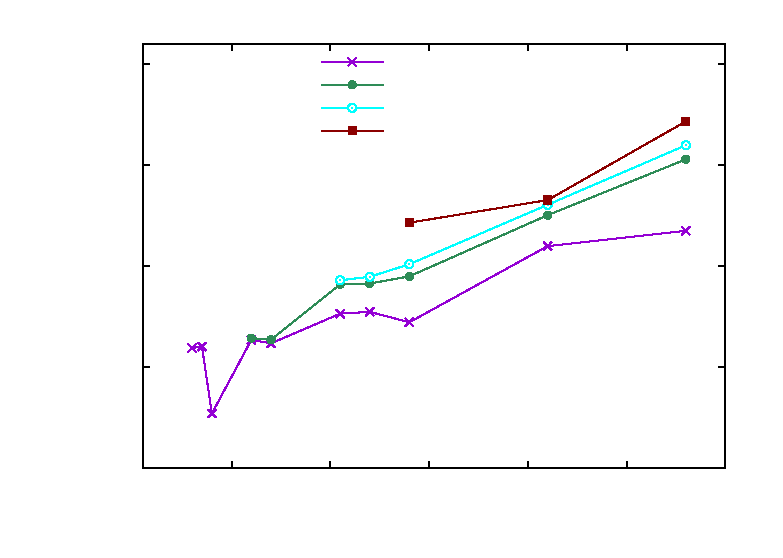
\includegraphics{plot-Tmult-nb_nogatherInt_11_500_selected_168}}%
    \gplfronttext
  \end{picture}%
\endgroup
}
      \caption{tempo di multicast dell implementazione SM con M=168 al variare del tempo di interarrivo}
      \label{fig:scalability_SM_size168}
    \end{subfigure}
    ~
    \begin{subfigure}[b]{\textwidth}
      \centering
      \addtocounter{subfigure}{-1}
      \renewcommand\thesubfigure{\alph{subfigure}3}
      \resizebox{\columnwidth}{!}{% GNUPLOT: LaTeX picture with Postscript
\begingroup
  \makeatletter
  \providecommand\color[2][]{%
    \GenericError{(gnuplot) \space\space\space\@spaces}{%
      Package color not loaded in conjunction with
      terminal option `colourtext'%
    }{See the gnuplot documentation for explanation.%
    }{Either use 'blacktext' in gnuplot or load the package
      color.sty in LaTeX.}%
    \renewcommand\color[2][]{}%
  }%
  \providecommand\includegraphics[2][]{%
    \GenericError{(gnuplot) \space\space\space\@spaces}{%
      Package graphicx or graphics not loaded%
    }{See the gnuplot documentation for explanation.%
    }{The gnuplot epslatex terminal needs graphicx.sty or graphics.sty.}%
    \renewcommand\includegraphics[2][]{}%
  }%
  \providecommand\rotatebox[2]{#2}%
  \@ifundefined{ifGPcolor}{%
    \newif\ifGPcolor
    \GPcolortrue
  }{}%
  \@ifundefined{ifGPblacktext}{%
    \newif\ifGPblacktext
    \GPblacktexttrue
  }{}%
  % define a \g@addto@macro without @ in the name:
  \let\gplgaddtomacro\g@addto@macro
  % define empty templates for all commands taking text:
  \gdef\gplbacktext{}%
  \gdef\gplfronttext{}%
  \makeatother
  \ifGPblacktext
    % no textcolor at all
    \def\colorrgb#1{}%
    \def\colorgray#1{}%
  \else
    % gray or color?
    \ifGPcolor
      \def\colorrgb#1{\color[rgb]{#1}}%
      \def\colorgray#1{\color[gray]{#1}}%
      \expandafter\def\csname LTw\endcsname{\color{white}}%
      \expandafter\def\csname LTb\endcsname{\color{black}}%
      \expandafter\def\csname LTa\endcsname{\color{black}}%
      \expandafter\def\csname LT0\endcsname{\color[rgb]{1,0,0}}%
      \expandafter\def\csname LT1\endcsname{\color[rgb]{0,1,0}}%
      \expandafter\def\csname LT2\endcsname{\color[rgb]{0,0,1}}%
      \expandafter\def\csname LT3\endcsname{\color[rgb]{1,0,1}}%
      \expandafter\def\csname LT4\endcsname{\color[rgb]{0,1,1}}%
      \expandafter\def\csname LT5\endcsname{\color[rgb]{1,1,0}}%
      \expandafter\def\csname LT6\endcsname{\color[rgb]{0,0,0}}%
      \expandafter\def\csname LT7\endcsname{\color[rgb]{1,0.3,0}}%
      \expandafter\def\csname LT8\endcsname{\color[rgb]{0.5,0.5,0.5}}%
    \else
      % gray
      \def\colorrgb#1{\color{black}}%
      \def\colorgray#1{\color[gray]{#1}}%
      \expandafter\def\csname LTw\endcsname{\color{white}}%
      \expandafter\def\csname LTb\endcsname{\color{black}}%
      \expandafter\def\csname LTa\endcsname{\color{black}}%
      \expandafter\def\csname LT0\endcsname{\color{black}}%
      \expandafter\def\csname LT1\endcsname{\color{black}}%
      \expandafter\def\csname LT2\endcsname{\color{black}}%
      \expandafter\def\csname LT3\endcsname{\color{black}}%
      \expandafter\def\csname LT4\endcsname{\color{black}}%
      \expandafter\def\csname LT5\endcsname{\color{black}}%
      \expandafter\def\csname LT6\endcsname{\color{black}}%
      \expandafter\def\csname LT7\endcsname{\color{black}}%
      \expandafter\def\csname LT8\endcsname{\color{black}}%
    \fi
  \fi
  \setlength{\unitlength}{0.0500bp}%
  \begin{picture}(7200.00,5040.00)%
    \gplgaddtomacro\gplbacktext{%
      \csname LTb\endcsname%
      \put(1078,704){\makebox(0,0)[r]{\strut{} 0}}%
      \put(1078,1673){\makebox(0,0)[r]{\strut{} 500}}%
      \put(1078,2643){\makebox(0,0)[r]{\strut{} 1000}}%
      \put(1078,3612){\makebox(0,0)[r]{\strut{} 1500}}%
      \put(1078,4581){\makebox(0,0)[r]{\strut{} 2000}}%
      \put(2063,484){\makebox(0,0){\strut{} 10}}%
      \put(3011,484){\makebox(0,0){\strut{} 20}}%
      \put(3959,484){\makebox(0,0){\strut{} 30}}%
      \put(4907,484){\makebox(0,0){\strut{} 40}}%
      \put(5855,484){\makebox(0,0){\strut{} 50}}%
      \put(6803,484){\makebox(0,0){\strut{} 60}}%
      \put(176,2739){\rotatebox{-270}{\makebox(0,0){\strut{}multicast service time}}}%
      \put(4006,154){\makebox(0,0){\strut{}$n$parallel degree}}%
    }%
    \gplgaddtomacro\gplfronttext{%
      \csname LTb\endcsname%
      \put(2794,4602){\makebox(0,0)[r]{\strut{}$T_A$ 250000 $\tau$}}%
      \csname LTb\endcsname%
      \put(2794,4382){\makebox(0,0)[r]{\strut{}$T_A$ 150000 $\tau$}}%
      \csname LTb\endcsname%
      \put(2794,4162){\makebox(0,0)[r]{\strut{}$T_A$ 100000 $\tau$}}%
      \csname LTb\endcsname%
      \put(2794,3942){\makebox(0,0)[r]{\strut{}$T_A$ 80000 $\tau$}}%
    }%
    \gplbacktext
    \put(0,0){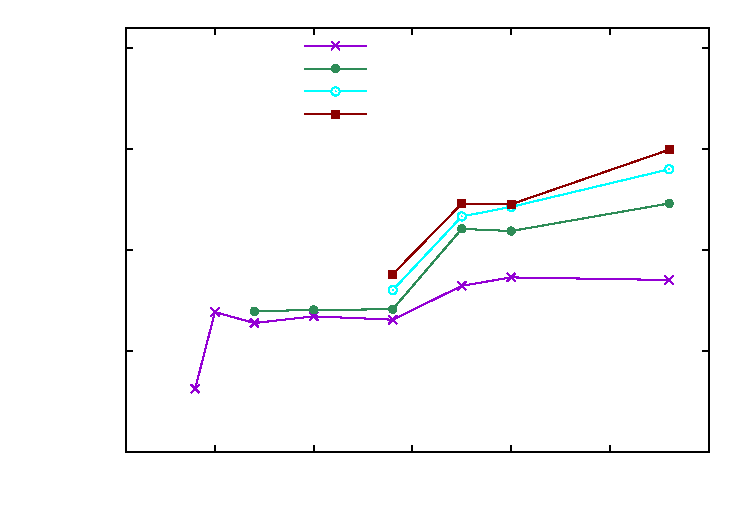
\includegraphics{plot-Tmult-nb_nogatherInt_11_500_selected_280}}%
    \gplfronttext
  \end{picture}%
\endgroup
}
      \caption{tempo di multicast dell implementazione SM con M=280 al variare del tempo di interarrivo}
      \label{fig:scalability_SM_size280}
    \end{subfigure}
    \label{fig:allscalability_SM}
  \end{subfigure}
\end{figure}

%%%%%%%%%%%%%%%%%%%%%%%%%%%%%%%%%%%%%%%%%%%%%%%%%%%%%%%%%%%%%%%%%%%%%%%%%%%%%%%%

%% \begin{figure}[p]
%%   \caption{Grafici del tempo di multicast al variare del tempo di interarrivo}
%%   \begin{subfigure}[b]{.5\columnwidth}
%%     \centering
%%     \renewcommand\thesubfigure{\alph{subfigure}}
%%     %% se vuoi spostare questa caption in fondo devi modificare anche i contatori!
%%     \caption{Implementazione con solo UDN}
%%     \begin{subfigure}[b]{\textwidth}
%%       \centering
%%       \addtocounter{subfigure}{-1}
%%       \renewcommand\thesubfigure{\alph{subfigure}1}
%%       \resizebox{\columnwidth}{!}{\input{plot1mlt_nogatherInt_00_500_selected_56.tex}}
%%       \caption{tempo di multicast dell implementazione UDN con M=56 al variare del tempo di interarrivo}
%%       \label{fig:scalability_UDN_size56}
%%     \end{subfigure}
%%     ~
%%     \begin{subfigure}[b]{\textwidth}
%%       \centering
%%       \addtocounter{subfigure}{-1}
%%       \renewcommand\thesubfigure{\alph{subfigure}2}
%%       \resizebox{\columnwidth}{!}{\input{plot1mlt_nogatherInt_00_500_selected_168.tex}}
%%       \caption{tempo di multicast dell implementazione UDN con M=168 al variare del tempo di interarrivo}
%%       \label{fig:scalability_UDN_size168}
%%     \end{subfigure}
%%     ~
%%     \begin{subfigure}[b]{\textwidth}
%%       \centering
%%       \addtocounter{subfigure}{-1}
%%       \renewcommand\thesubfigure{\alph{subfigure}3}
%%       \resizebox{\columnwidth}{!}{\input{plot1mlt_nogatherInt_00_500_selected_280.tex}}
%%       \caption{tempo di multicast dell implementazione UDN con M=280 al variare del tempo di interarrivo}
%%       \label{fig:scalability_UDN_size280}
%%     \end{subfigure}
%%     \label{fig:allScalbility_UDN}
%%   \end{subfigure}
%%   \hspace{2ex}
%%   \begin{subfigure}[b]{.5\columnwidth}
%%     \centering
%%     \renewcommand\thesubfigure{\alph{subfigure}}
%%     \caption{Implementazione con solo SM}
%%     \begin{subfigure}[b]{\textwidth}
%%       \centering
%%       \addtocounter{subfigure}{-1}
%%       \renewcommand\thesubfigure{\alph{subfigure}1}
%%       \resizebox{\columnwidth}{!}{\input{plot1mlt_nogatherInt_11_500_selected_56.tex}}
%%       \caption{tempo di multicast dell implementazione SM con M=56 al variare del tempo di interarrivo}
%%       \label{fig:scalability_SM_size56}
%%     \end{subfigure}
%%     ~
%%     \begin{subfigure}[b]{\textwidth}
%%       \centering
%%       \addtocounter{subfigure}{-1}
%%       \renewcommand\thesubfigure{\alph{subfigure}2}
%%       \resizebox{\columnwidth}{!}{\input{plot1mlt_nogatherInt_11_500_selected_168.tex}}
%%       \caption{tempo di multicast dell implementazione SM con M=168 al variare del tempo di interarrivo}
%%       \label{fig:scalability_SM_size168}
%%     \end{subfigure}
%%     ~
%%     \begin{subfigure}[b]{\textwidth}
%%       \centering
%%       \addtocounter{subfigure}{-1}
%%       \renewcommand\thesubfigure{\alph{subfigure}3}
%%       \resizebox{\columnwidth}{!}{\input{plot1mlt_nogatherInt_11_500_selected_280.tex}}
%%       \caption{tempo di multicast dell implementazione SM con M=280 al variare del tempo di interarrivo}
%%       \label{fig:scalability_SM_size280}
%%     \end{subfigure}
%%     \label{fig:allscalability_SM}
%%   \end{subfigure}
%% \end{figure}

%% %%%%%%%%%%%%%%%%%%%%%%%%%%%%%%%%%%%%%%%%%%%%%%%%%%%%%%%%%%%%%%%%%%%%%%%%%%%%%%%%

%% \begin{figure}[p]
%%   \caption{Grafici del tempo di multicast al variare del tempo di interarrivo}
%%   \begin{subfigure}[b]{.5\columnwidth}
%%     \centering
%%     \renewcommand\thesubfigure{\alph{subfigure}}
%%     %% se vuoi spostare questa caption in fondo devi modificare anche i contatori!
%%     \caption{Implementazione con solo UDN}
%%     \begin{subfigure}[b]{\textwidth}
%%       \centering
%%       \addtocounter{subfigure}{-1}
%%       \renewcommand\thesubfigure{\alph{subfigure}1}
%%       \resizebox{\columnwidth}{!}{\input{plot1mlt_nogatherInt_00_500_selected_56.tex}}
%%       \caption{tempo di multicast dell implementazione UDN con M=56 al variare del tempo di interarrivo}
%%       \label{fig:scalability_UDN_size56}
%%     \end{subfigure}
%%     ~
%%     \begin{subfigure}[b]{\textwidth}
%%       \centering
%%       \addtocounter{subfigure}{-1}
%%       \renewcommand\thesubfigure{\alph{subfigure}2}
%%       \resizebox{\columnwidth}{!}{\input{plot1mlt_nogatherInt_00_500_selected_168.tex}}
%%       \caption{tempo di multicast dell implementazione UDN con M=168 al variare del tempo di interarrivo}
%%       \label{fig:scalability_UDN_size168}
%%     \end{subfigure}
%%     ~
%%     \begin{subfigure}[b]{\textwidth}
%%       \centering
%%       \addtocounter{subfigure}{-1}
%%       \renewcommand\thesubfigure{\alph{subfigure}3}
%%       \resizebox{\columnwidth}{!}{\input{plot1mlt_nogatherInt_00_500_selected_280.tex}}
%%       \caption{tempo di multicast dell implementazione UDN con M=280 al variare del tempo di interarrivo}
%%       \label{fig:scalability_UDN_size280}
%%     \end{subfigure}
%%     \label{fig:allScalbility_UDN}
%%   \end{subfigure}
%%   \hspace{2ex}
%%   \begin{subfigure}[b]{.5\columnwidth}
%%     \centering
%%     \renewcommand\thesubfigure{\alph{subfigure}}
%%     \caption{Implementazione con solo SM}
%%     \begin{subfigure}[b]{\textwidth}
%%       \centering
%%       \addtocounter{subfigure}{-1}
%%       \renewcommand\thesubfigure{\alph{subfigure}1}
%%       \resizebox{\columnwidth}{!}{\input{plot1mlt_nogatherInt_01_500_selected_56.tex}}
%%       \caption{tempo di multicast dell implementazione SM con M=56 al variare del tempo di interarrivo}
%%       \label{fig:scalability_SM_size56}
%%     \end{subfigure}
%%     ~
%%     \begin{subfigure}[b]{\textwidth}
%%       \centering
%%       \addtocounter{subfigure}{-1}
%%       \renewcommand\thesubfigure{\alph{subfigure}2}
%%       \resizebox{\columnwidth}{!}{\input{plot1mlt_nogatherInt_01_500_selected_168.tex}}
%%       \caption{tempo di multicast dell implementazione SM con M=168 al variare del tempo di interarrivo}
%%       \label{fig:scalability_SM_size168}
%%     \end{subfigure}
%%     ~
%%     \begin{subfigure}[b]{\textwidth}
%%       \centering
%%       \addtocounter{subfigure}{-1}
%%       \renewcommand\thesubfigure{\alph{subfigure}3}
%%       \resizebox{\columnwidth}{!}{\input{plot1mlt_nogatherInt_01_500_selected_280.tex}}
%%       \caption{tempo di multicast dell implementazione SM con M=280 al variare del tempo di interarrivo}
%%       \label{fig:scalability_SM_size280}
%%     \end{subfigure}
%%     \label{fig:allscalability_SM}
%%   \end{subfigure}
%% \end{figure}



%%%%%%%%%%%%%%%%%%%%%%%%%%%%%%%%%%%%%%%%%%%%%%%%%%%%%%%%%%%%%%%%%%%%%%%%%%%%%%%%

\newpage
\FloatBarrier
\subsection{Confronto scalabilit\`a delle due implementazioni}

\begin{figure}[h]
  \centering
  \begin{subfigure}[b]{.31\textheight}
    \centering
    \resizebox{\columnwidth}{!}{% GNUPLOT: LaTeX picture with Postscript
\begingroup
  \makeatletter
  \providecommand\color[2][]{%
    \GenericError{(gnuplot) \space\space\space\@spaces}{%
      Package color not loaded in conjunction with
      terminal option `colourtext'%
    }{See the gnuplot documentation for explanation.%
    }{Either use 'blacktext' in gnuplot or load the package
      color.sty in LaTeX.}%
    \renewcommand\color[2][]{}%
  }%
  \providecommand\includegraphics[2][]{%
    \GenericError{(gnuplot) \space\space\space\@spaces}{%
      Package graphicx or graphics not loaded%
    }{See the gnuplot documentation for explanation.%
    }{The gnuplot epslatex terminal needs graphicx.sty or graphics.sty.}%
    \renewcommand\includegraphics[2][]{}%
  }%
  \providecommand\rotatebox[2]{#2}%
  \@ifundefined{ifGPcolor}{%
    \newif\ifGPcolor
    \GPcolortrue
  }{}%
  \@ifundefined{ifGPblacktext}{%
    \newif\ifGPblacktext
    \GPblacktexttrue
  }{}%
  % define a \g@addto@macro without @ in the name:
  \let\gplgaddtomacro\g@addto@macro
  % define empty templates for all commands taking text:
  \gdef\gplbacktext{}%
  \gdef\gplfronttext{}%
  \makeatother
  \ifGPblacktext
    % no textcolor at all
    \def\colorrgb#1{}%
    \def\colorgray#1{}%
  \else
    % gray or color?
    \ifGPcolor
      \def\colorrgb#1{\color[rgb]{#1}}%
      \def\colorgray#1{\color[gray]{#1}}%
      \expandafter\def\csname LTw\endcsname{\color{white}}%
      \expandafter\def\csname LTb\endcsname{\color{black}}%
      \expandafter\def\csname LTa\endcsname{\color{black}}%
      \expandafter\def\csname LT0\endcsname{\color[rgb]{1,0,0}}%
      \expandafter\def\csname LT1\endcsname{\color[rgb]{0,1,0}}%
      \expandafter\def\csname LT2\endcsname{\color[rgb]{0,0,1}}%
      \expandafter\def\csname LT3\endcsname{\color[rgb]{1,0,1}}%
      \expandafter\def\csname LT4\endcsname{\color[rgb]{0,1,1}}%
      \expandafter\def\csname LT5\endcsname{\color[rgb]{1,1,0}}%
      \expandafter\def\csname LT6\endcsname{\color[rgb]{0,0,0}}%
      \expandafter\def\csname LT7\endcsname{\color[rgb]{1,0.3,0}}%
      \expandafter\def\csname LT8\endcsname{\color[rgb]{0.5,0.5,0.5}}%
    \else
      % gray
      \def\colorrgb#1{\color{black}}%
      \def\colorgray#1{\color[gray]{#1}}%
      \expandafter\def\csname LTw\endcsname{\color{white}}%
      \expandafter\def\csname LTb\endcsname{\color{black}}%
      \expandafter\def\csname LTa\endcsname{\color{black}}%
      \expandafter\def\csname LT0\endcsname{\color{black}}%
      \expandafter\def\csname LT1\endcsname{\color{black}}%
      \expandafter\def\csname LT2\endcsname{\color{black}}%
      \expandafter\def\csname LT3\endcsname{\color{black}}%
      \expandafter\def\csname LT4\endcsname{\color{black}}%
      \expandafter\def\csname LT5\endcsname{\color{black}}%
      \expandafter\def\csname LT6\endcsname{\color{black}}%
      \expandafter\def\csname LT7\endcsname{\color{black}}%
      \expandafter\def\csname LT8\endcsname{\color{black}}%
    \fi
  \fi
  \setlength{\unitlength}{0.0500bp}%
  \begin{picture}(7200.00,5040.00)%
    \gplgaddtomacro\gplbacktext{%
      \csname LTb\endcsname%
      \put(814,1325){\makebox(0,0)[r]{\strut{} 10}}%
      \put(814,2015){\makebox(0,0)[r]{\strut{} 20}}%
      \put(814,2705){\makebox(0,0)[r]{\strut{} 30}}%
      \put(814,3395){\makebox(0,0)[r]{\strut{} 40}}%
      \put(814,4085){\makebox(0,0)[r]{\strut{} 50}}%
      \put(814,4775){\makebox(0,0)[r]{\strut{} 60}}%
      \put(1839,484){\makebox(0,0){\strut{} 10}}%
      \put(2832,484){\makebox(0,0){\strut{} 20}}%
      \put(3825,484){\makebox(0,0){\strut{} 30}}%
      \put(4818,484){\makebox(0,0){\strut{} 40}}%
      \put(5810,484){\makebox(0,0){\strut{} 50}}%
      \put(6803,484){\makebox(0,0){\strut{} 60}}%
      \put(176,2739){\rotatebox{-270}{\makebox(0,0){\strut{}scalability}}}%
      \put(3874,154){\makebox(0,0){\strut{}$n$ parallel degree}}%
    }%
    \gplgaddtomacro\gplfronttext{%
      \csname LTb\endcsname%
      \put(3322,4602){\makebox(0,0)[r]{\strut{}ideal scalability}}%
      \csname LTb\endcsname%
      \put(3322,4382){\makebox(0,0)[r]{\strut{}udn udn}}%
      \csname LTb\endcsname%
      \put(3322,4162){\makebox(0,0)[r]{\strut{}sm sm}}%
    }%
    \gplbacktext
    \put(0,0){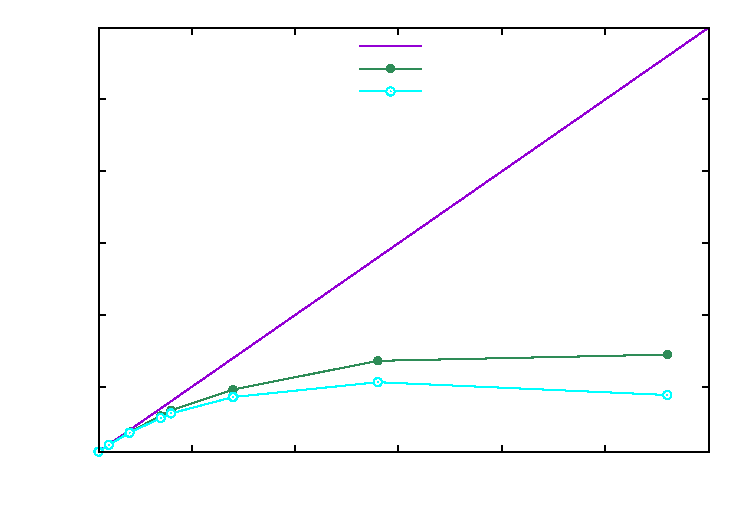
\includegraphics{plot-comp-Tc-s_nogatherInt_all_500_181_56}}%
    \gplfronttext
  \end{picture}%
\endgroup
}
    \caption{Confronto della scalabilita nelle diverse implementazioni, Ta=181, M=56}
  \end{subfigure}
  \vfill
  %%\vspace{5ex}
  \begin{subfigure}[b]{.31\textheight}
    \centering
    \resizebox{\columnwidth}{!}{% GNUPLOT: LaTeX picture with Postscript
\begingroup
  \makeatletter
  \providecommand\color[2][]{%
    \GenericError{(gnuplot) \space\space\space\@spaces}{%
      Package color not loaded in conjunction with
      terminal option `colourtext'%
    }{See the gnuplot documentation for explanation.%
    }{Either use 'blacktext' in gnuplot or load the package
      color.sty in LaTeX.}%
    \renewcommand\color[2][]{}%
  }%
  \providecommand\includegraphics[2][]{%
    \GenericError{(gnuplot) \space\space\space\@spaces}{%
      Package graphicx or graphics not loaded%
    }{See the gnuplot documentation for explanation.%
    }{The gnuplot epslatex terminal needs graphicx.sty or graphics.sty.}%
    \renewcommand\includegraphics[2][]{}%
  }%
  \providecommand\rotatebox[2]{#2}%
  \@ifundefined{ifGPcolor}{%
    \newif\ifGPcolor
    \GPcolortrue
  }{}%
  \@ifundefined{ifGPblacktext}{%
    \newif\ifGPblacktext
    \GPblacktexttrue
  }{}%
  % define a \g@addto@macro without @ in the name:
  \let\gplgaddtomacro\g@addto@macro
  % define empty templates for all commands taking text:
  \gdef\gplbacktext{}%
  \gdef\gplfronttext{}%
  \makeatother
  \ifGPblacktext
    % no textcolor at all
    \def\colorrgb#1{}%
    \def\colorgray#1{}%
  \else
    % gray or color?
    \ifGPcolor
      \def\colorrgb#1{\color[rgb]{#1}}%
      \def\colorgray#1{\color[gray]{#1}}%
      \expandafter\def\csname LTw\endcsname{\color{white}}%
      \expandafter\def\csname LTb\endcsname{\color{black}}%
      \expandafter\def\csname LTa\endcsname{\color{black}}%
      \expandafter\def\csname LT0\endcsname{\color[rgb]{1,0,0}}%
      \expandafter\def\csname LT1\endcsname{\color[rgb]{0,1,0}}%
      \expandafter\def\csname LT2\endcsname{\color[rgb]{0,0,1}}%
      \expandafter\def\csname LT3\endcsname{\color[rgb]{1,0,1}}%
      \expandafter\def\csname LT4\endcsname{\color[rgb]{0,1,1}}%
      \expandafter\def\csname LT5\endcsname{\color[rgb]{1,1,0}}%
      \expandafter\def\csname LT6\endcsname{\color[rgb]{0,0,0}}%
      \expandafter\def\csname LT7\endcsname{\color[rgb]{1,0.3,0}}%
      \expandafter\def\csname LT8\endcsname{\color[rgb]{0.5,0.5,0.5}}%
    \else
      % gray
      \def\colorrgb#1{\color{black}}%
      \def\colorgray#1{\color[gray]{#1}}%
      \expandafter\def\csname LTw\endcsname{\color{white}}%
      \expandafter\def\csname LTb\endcsname{\color{black}}%
      \expandafter\def\csname LTa\endcsname{\color{black}}%
      \expandafter\def\csname LT0\endcsname{\color{black}}%
      \expandafter\def\csname LT1\endcsname{\color{black}}%
      \expandafter\def\csname LT2\endcsname{\color{black}}%
      \expandafter\def\csname LT3\endcsname{\color{black}}%
      \expandafter\def\csname LT4\endcsname{\color{black}}%
      \expandafter\def\csname LT5\endcsname{\color{black}}%
      \expandafter\def\csname LT6\endcsname{\color{black}}%
      \expandafter\def\csname LT7\endcsname{\color{black}}%
      \expandafter\def\csname LT8\endcsname{\color{black}}%
    \fi
  \fi
  \setlength{\unitlength}{0.0500bp}%
  \begin{picture}(7200.00,5040.00)%
    \gplgaddtomacro\gplbacktext{%
      \csname LTb\endcsname%
      \put(814,1325){\makebox(0,0)[r]{\strut{} 10}}%
      \put(814,2015){\makebox(0,0)[r]{\strut{} 20}}%
      \put(814,2705){\makebox(0,0)[r]{\strut{} 30}}%
      \put(814,3395){\makebox(0,0)[r]{\strut{} 40}}%
      \put(814,4085){\makebox(0,0)[r]{\strut{} 50}}%
      \put(814,4775){\makebox(0,0)[r]{\strut{} 60}}%
      \put(1839,484){\makebox(0,0){\strut{} 10}}%
      \put(2832,484){\makebox(0,0){\strut{} 20}}%
      \put(3825,484){\makebox(0,0){\strut{} 30}}%
      \put(4818,484){\makebox(0,0){\strut{} 40}}%
      \put(5810,484){\makebox(0,0){\strut{} 50}}%
      \put(6803,484){\makebox(0,0){\strut{} 60}}%
      \put(176,2739){\rotatebox{-270}{\makebox(0,0){\strut{}scalability}}}%
      \put(3874,154){\makebox(0,0){\strut{}$n$ parallel degree}}%
    }%
    \gplgaddtomacro\gplfronttext{%
      \csname LTb\endcsname%
      \put(3322,4602){\makebox(0,0)[r]{\strut{}ideal scalability}}%
      \csname LTb\endcsname%
      \put(3322,4382){\makebox(0,0)[r]{\strut{}udn udn}}%
      \csname LTb\endcsname%
      \put(3322,4162){\makebox(0,0)[r]{\strut{}sm sm}}%
    }%
    \gplbacktext
    \put(0,0){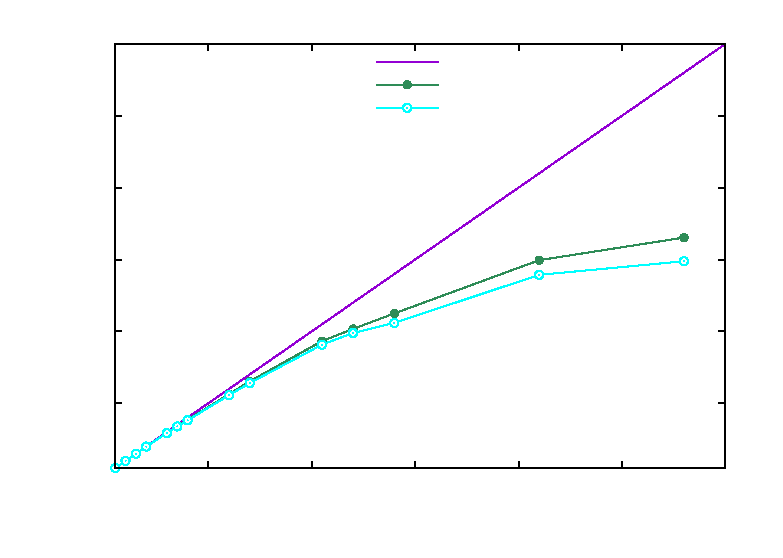
\includegraphics{plot-comp-Tc-s_nogatherInt_all_500_181_168}}%
    \gplfronttext
  \end{picture}%
\endgroup
}
    \caption{Confronto della scalabilita nelle diverse implementazioni, Ta=181, M=168}
  \end{subfigure}
  \vfill
  \begin{subfigure}[b]{.31\textheight}
    \centering
    \resizebox{\columnwidth}{!}{% GNUPLOT: LaTeX picture with Postscript
\begingroup
  \makeatletter
  \providecommand\color[2][]{%
    \GenericError{(gnuplot) \space\space\space\@spaces}{%
      Package color not loaded in conjunction with
      terminal option `colourtext'%
    }{See the gnuplot documentation for explanation.%
    }{Either use 'blacktext' in gnuplot or load the package
      color.sty in LaTeX.}%
    \renewcommand\color[2][]{}%
  }%
  \providecommand\includegraphics[2][]{%
    \GenericError{(gnuplot) \space\space\space\@spaces}{%
      Package graphicx or graphics not loaded%
    }{See the gnuplot documentation for explanation.%
    }{The gnuplot epslatex terminal needs graphicx.sty or graphics.sty.}%
    \renewcommand\includegraphics[2][]{}%
  }%
  \providecommand\rotatebox[2]{#2}%
  \@ifundefined{ifGPcolor}{%
    \newif\ifGPcolor
    \GPcolortrue
  }{}%
  \@ifundefined{ifGPblacktext}{%
    \newif\ifGPblacktext
    \GPblacktexttrue
  }{}%
  % define a \g@addto@macro without @ in the name:
  \let\gplgaddtomacro\g@addto@macro
  % define empty templates for all commands taking text:
  \gdef\gplbacktext{}%
  \gdef\gplfronttext{}%
  \makeatother
  \ifGPblacktext
    % no textcolor at all
    \def\colorrgb#1{}%
    \def\colorgray#1{}%
  \else
    % gray or color?
    \ifGPcolor
      \def\colorrgb#1{\color[rgb]{#1}}%
      \def\colorgray#1{\color[gray]{#1}}%
      \expandafter\def\csname LTw\endcsname{\color{white}}%
      \expandafter\def\csname LTb\endcsname{\color{black}}%
      \expandafter\def\csname LTa\endcsname{\color{black}}%
      \expandafter\def\csname LT0\endcsname{\color[rgb]{1,0,0}}%
      \expandafter\def\csname LT1\endcsname{\color[rgb]{0,1,0}}%
      \expandafter\def\csname LT2\endcsname{\color[rgb]{0,0,1}}%
      \expandafter\def\csname LT3\endcsname{\color[rgb]{1,0,1}}%
      \expandafter\def\csname LT4\endcsname{\color[rgb]{0,1,1}}%
      \expandafter\def\csname LT5\endcsname{\color[rgb]{1,1,0}}%
      \expandafter\def\csname LT6\endcsname{\color[rgb]{0,0,0}}%
      \expandafter\def\csname LT7\endcsname{\color[rgb]{1,0.3,0}}%
      \expandafter\def\csname LT8\endcsname{\color[rgb]{0.5,0.5,0.5}}%
    \else
      % gray
      \def\colorrgb#1{\color{black}}%
      \def\colorgray#1{\color[gray]{#1}}%
      \expandafter\def\csname LTw\endcsname{\color{white}}%
      \expandafter\def\csname LTb\endcsname{\color{black}}%
      \expandafter\def\csname LTa\endcsname{\color{black}}%
      \expandafter\def\csname LT0\endcsname{\color{black}}%
      \expandafter\def\csname LT1\endcsname{\color{black}}%
      \expandafter\def\csname LT2\endcsname{\color{black}}%
      \expandafter\def\csname LT3\endcsname{\color{black}}%
      \expandafter\def\csname LT4\endcsname{\color{black}}%
      \expandafter\def\csname LT5\endcsname{\color{black}}%
      \expandafter\def\csname LT6\endcsname{\color{black}}%
      \expandafter\def\csname LT7\endcsname{\color{black}}%
      \expandafter\def\csname LT8\endcsname{\color{black}}%
    \fi
  \fi
  \setlength{\unitlength}{0.0500bp}%
  \begin{picture}(7200.00,5040.00)%
    \gplgaddtomacro\gplbacktext{%
      \csname LTb\endcsname%
      \put(814,1325){\makebox(0,0)[r]{\strut{} 10}}%
      \put(814,2015){\makebox(0,0)[r]{\strut{} 20}}%
      \put(814,2705){\makebox(0,0)[r]{\strut{} 30}}%
      \put(814,3395){\makebox(0,0)[r]{\strut{} 40}}%
      \put(814,4085){\makebox(0,0)[r]{\strut{} 50}}%
      \put(814,4775){\makebox(0,0)[r]{\strut{} 60}}%
      \put(1839,484){\makebox(0,0){\strut{} 10}}%
      \put(2832,484){\makebox(0,0){\strut{} 20}}%
      \put(3825,484){\makebox(0,0){\strut{} 30}}%
      \put(4818,484){\makebox(0,0){\strut{} 40}}%
      \put(5810,484){\makebox(0,0){\strut{} 50}}%
      \put(6803,484){\makebox(0,0){\strut{} 60}}%
      \put(176,2739){\rotatebox{-270}{\makebox(0,0){\strut{}scalability}}}%
      \put(3874,154){\makebox(0,0){\strut{}$n$ parallel degree}}%
    }%
    \gplgaddtomacro\gplfronttext{%
      \csname LTb\endcsname%
      \put(3322,4602){\makebox(0,0)[r]{\strut{}ideal scalability}}%
      \csname LTb\endcsname%
      \put(3322,4382){\makebox(0,0)[r]{\strut{}udn udn}}%
      \csname LTb\endcsname%
      \put(3322,4162){\makebox(0,0)[r]{\strut{}sm sm}}%
    }%
    \gplbacktext
    \put(0,0){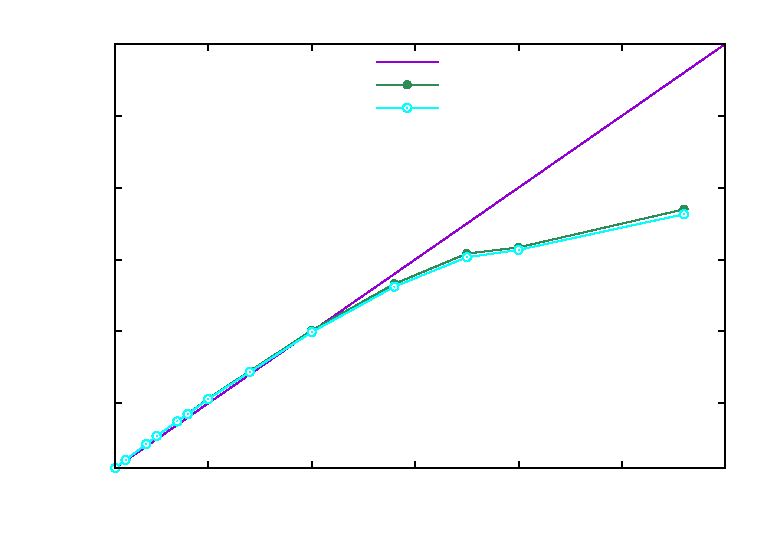
\includegraphics{plot-comp-Tc-s_nogatherInt_all_500_181_280}}%
    \gplfronttext
  \end{picture}%
\endgroup
}
    \caption{Confronto della scalabilita nelle diverse implementazioni, Ta=181, M=280}
  \end{subfigure}
\end{figure}

\FloatBarrier


%%%%%%%%%%%%%%%%%%%%%%%%%%%%%%%%%%%%%%%%%%%%%%%%%%%%%%%%%%%%%%%%%%%%%%%%%%%%%%%%

\newpage
\FloatBarrier
\subsection{Row calculation time}

\begin{figure}[h]
  \caption{Rapporto tra i tempi di calcolo di un singolo prodotto scalare}
  \begin{subfigure}[b]{.5\textwidth}
    \centering
    \resizebox{\columnwidth}{!}{% GNUPLOT: LaTeX picture with Postscript
\begingroup
  \makeatletter
  \providecommand\color[2][]{%
    \GenericError{(gnuplot) \space\space\space\@spaces}{%
      Package color not loaded in conjunction with
      terminal option `colourtext'%
    }{See the gnuplot documentation for explanation.%
    }{Either use 'blacktext' in gnuplot or load the package
      color.sty in LaTeX.}%
    \renewcommand\color[2][]{}%
  }%
  \providecommand\includegraphics[2][]{%
    \GenericError{(gnuplot) \space\space\space\@spaces}{%
      Package graphicx or graphics not loaded%
    }{See the gnuplot documentation for explanation.%
    }{The gnuplot epslatex terminal needs graphicx.sty or graphics.sty.}%
    \renewcommand\includegraphics[2][]{}%
  }%
  \providecommand\rotatebox[2]{#2}%
  \@ifundefined{ifGPcolor}{%
    \newif\ifGPcolor
    \GPcolortrue
  }{}%
  \@ifundefined{ifGPblacktext}{%
    \newif\ifGPblacktext
    \GPblacktextfalse
  }{}%
  % define a \g@addto@macro without @ in the name:
  \let\gplgaddtomacro\g@addto@macro
  % define empty templates for all commands taking text:
  \gdef\gplbacktext{}%
  \gdef\gplfronttext{}%
  \makeatother
  \ifGPblacktext
    % no textcolor at all
    \def\colorrgb#1{}%
    \def\colorgray#1{}%
  \else
    % gray or color?
    \ifGPcolor
      \def\colorrgb#1{\color[rgb]{#1}}%
      \def\colorgray#1{\color[gray]{#1}}%
      \expandafter\def\csname LTw\endcsname{\color{white}}%
      \expandafter\def\csname LTb\endcsname{\color{black}}%
      \expandafter\def\csname LTa\endcsname{\color{black}}%
      \expandafter\def\csname LT0\endcsname{\color[rgb]{1,0,0}}%
      \expandafter\def\csname LT1\endcsname{\color[rgb]{0,1,0}}%
      \expandafter\def\csname LT2\endcsname{\color[rgb]{0,0,1}}%
      \expandafter\def\csname LT3\endcsname{\color[rgb]{1,0,1}}%
      \expandafter\def\csname LT4\endcsname{\color[rgb]{0,1,1}}%
      \expandafter\def\csname LT5\endcsname{\color[rgb]{1,1,0}}%
      \expandafter\def\csname LT6\endcsname{\color[rgb]{0,0,0}}%
      \expandafter\def\csname LT7\endcsname{\color[rgb]{1,0.3,0}}%
      \expandafter\def\csname LT8\endcsname{\color[rgb]{0.5,0.5,0.5}}%
    \else
      % gray
      \def\colorrgb#1{\color{black}}%
      \def\colorgray#1{\color[gray]{#1}}%
      \expandafter\def\csname LTw\endcsname{\color{white}}%
      \expandafter\def\csname LTb\endcsname{\color{black}}%
      \expandafter\def\csname LTa\endcsname{\color{black}}%
      \expandafter\def\csname LT0\endcsname{\color{black}}%
      \expandafter\def\csname LT1\endcsname{\color{black}}%
      \expandafter\def\csname LT2\endcsname{\color{black}}%
      \expandafter\def\csname LT3\endcsname{\color{black}}%
      \expandafter\def\csname LT4\endcsname{\color{black}}%
      \expandafter\def\csname LT5\endcsname{\color{black}}%
      \expandafter\def\csname LT6\endcsname{\color{black}}%
      \expandafter\def\csname LT7\endcsname{\color{black}}%
      \expandafter\def\csname LT8\endcsname{\color{black}}%
    \fi
  \fi
  \setlength{\unitlength}{0.0500bp}%
  \begin{picture}(7200.00,5040.00)%
    \gplgaddtomacro\gplbacktext{%
      \csname LTb\endcsname%
      \put(946,1074){\makebox(0,0)[r]{\strut{} 1}}%
      \csname LTb\endcsname%
      \put(946,1999){\makebox(0,0)[r]{\strut{} 1.5}}%
      \csname LTb\endcsname%
      \put(946,2925){\makebox(0,0)[r]{\strut{} 2}}%
      \csname LTb\endcsname%
      \put(946,3850){\makebox(0,0)[r]{\strut{} 2.5}}%
      \csname LTb\endcsname%
      \put(946,4775){\makebox(0,0)[r]{\strut{} 3}}%
      \csname LTb\endcsname%
      \put(1951,484){\makebox(0,0){\strut{} 10}}%
      \csname LTb\endcsname%
      \put(2922,484){\makebox(0,0){\strut{} 20}}%
      \csname LTb\endcsname%
      \put(3892,484){\makebox(0,0){\strut{} 30}}%
      \csname LTb\endcsname%
      \put(4862,484){\makebox(0,0){\strut{} 40}}%
      \csname LTb\endcsname%
      \put(5833,484){\makebox(0,0){\strut{} 50}}%
      \csname LTb\endcsname%
      \put(6803,484){\makebox(0,0){\strut{} 60}}%
      \put(176,2739){\rotatebox{-270}{\makebox(0,0){\strut{}$T_{\textrm{row}}^{\phantom{row}(n)} / T_{\textrm{row}}^{\phantom{row}(1)}$}}}%
      \put(3940,154){\makebox(0,0){\strut{}$n$ parallel degree}}%
    }%
    \gplgaddtomacro\gplfronttext{%
      \csname LTb\endcsname%
      \put(3718,4602){\makebox(0,0)[r]{\strut{}Matrix Size 280x280}}%
      \csname LTb\endcsname%
      \put(3718,4382){\makebox(0,0)[r]{\strut{}Matrix Size 168x168}}%
      \csname LTb\endcsname%
      \put(3718,4162){\makebox(0,0)[r]{\strut{}Matrix Size 56x56}}%
    }%
    \gplbacktext
    \put(0,0){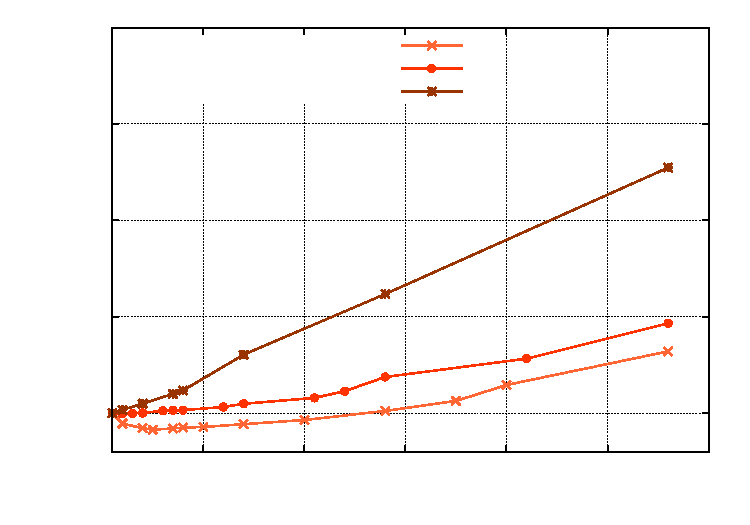
\includegraphics{plot-rowCalcT_nogatherInt_00_500_4000_all}}%
    \gplfronttext
  \end{picture}%
\endgroup
}
    \caption{Tempi di calcolo di una singola Row $\cdot$ Col con Ta=4000, canali UDN e dati Int}
  \end{subfigure}
  \hspace{2ex}
  \begin{subfigure}[b]{.5\textwidth}
    \centering
    \resizebox{\columnwidth}{!}{% GNUPLOT: LaTeX picture with Postscript
\begingroup
  \makeatletter
  \providecommand\color[2][]{%
    \GenericError{(gnuplot) \space\space\space\@spaces}{%
      Package color not loaded in conjunction with
      terminal option `colourtext'%
    }{See the gnuplot documentation for explanation.%
    }{Either use 'blacktext' in gnuplot or load the package
      color.sty in LaTeX.}%
    \renewcommand\color[2][]{}%
  }%
  \providecommand\includegraphics[2][]{%
    \GenericError{(gnuplot) \space\space\space\@spaces}{%
      Package graphicx or graphics not loaded%
    }{See the gnuplot documentation for explanation.%
    }{The gnuplot epslatex terminal needs graphicx.sty or graphics.sty.}%
    \renewcommand\includegraphics[2][]{}%
  }%
  \providecommand\rotatebox[2]{#2}%
  \@ifundefined{ifGPcolor}{%
    \newif\ifGPcolor
    \GPcolortrue
  }{}%
  \@ifundefined{ifGPblacktext}{%
    \newif\ifGPblacktext
    \GPblacktextfalse
  }{}%
  % define a \g@addto@macro without @ in the name:
  \let\gplgaddtomacro\g@addto@macro
  % define empty templates for all commands taking text:
  \gdef\gplbacktext{}%
  \gdef\gplfronttext{}%
  \makeatother
  \ifGPblacktext
    % no textcolor at all
    \def\colorrgb#1{}%
    \def\colorgray#1{}%
  \else
    % gray or color?
    \ifGPcolor
      \def\colorrgb#1{\color[rgb]{#1}}%
      \def\colorgray#1{\color[gray]{#1}}%
      \expandafter\def\csname LTw\endcsname{\color{white}}%
      \expandafter\def\csname LTb\endcsname{\color{black}}%
      \expandafter\def\csname LTa\endcsname{\color{black}}%
      \expandafter\def\csname LT0\endcsname{\color[rgb]{1,0,0}}%
      \expandafter\def\csname LT1\endcsname{\color[rgb]{0,1,0}}%
      \expandafter\def\csname LT2\endcsname{\color[rgb]{0,0,1}}%
      \expandafter\def\csname LT3\endcsname{\color[rgb]{1,0,1}}%
      \expandafter\def\csname LT4\endcsname{\color[rgb]{0,1,1}}%
      \expandafter\def\csname LT5\endcsname{\color[rgb]{1,1,0}}%
      \expandafter\def\csname LT6\endcsname{\color[rgb]{0,0,0}}%
      \expandafter\def\csname LT7\endcsname{\color[rgb]{1,0.3,0}}%
      \expandafter\def\csname LT8\endcsname{\color[rgb]{0.5,0.5,0.5}}%
    \else
      % gray
      \def\colorrgb#1{\color{black}}%
      \def\colorgray#1{\color[gray]{#1}}%
      \expandafter\def\csname LTw\endcsname{\color{white}}%
      \expandafter\def\csname LTb\endcsname{\color{black}}%
      \expandafter\def\csname LTa\endcsname{\color{black}}%
      \expandafter\def\csname LT0\endcsname{\color{black}}%
      \expandafter\def\csname LT1\endcsname{\color{black}}%
      \expandafter\def\csname LT2\endcsname{\color{black}}%
      \expandafter\def\csname LT3\endcsname{\color{black}}%
      \expandafter\def\csname LT4\endcsname{\color{black}}%
      \expandafter\def\csname LT5\endcsname{\color{black}}%
      \expandafter\def\csname LT6\endcsname{\color{black}}%
      \expandafter\def\csname LT7\endcsname{\color{black}}%
      \expandafter\def\csname LT8\endcsname{\color{black}}%
    \fi
  \fi
  \setlength{\unitlength}{0.0500bp}%
  \begin{picture}(7200.00,5040.00)%
    \gplgaddtomacro\gplbacktext{%
      \csname LTb\endcsname%
      \put(946,1074){\makebox(0,0)[r]{\strut{} 1}}%
      \csname LTb\endcsname%
      \put(946,1999){\makebox(0,0)[r]{\strut{} 1.5}}%
      \csname LTb\endcsname%
      \put(946,2925){\makebox(0,0)[r]{\strut{} 2}}%
      \csname LTb\endcsname%
      \put(946,3850){\makebox(0,0)[r]{\strut{} 2.5}}%
      \csname LTb\endcsname%
      \put(946,4775){\makebox(0,0)[r]{\strut{} 3}}%
      \csname LTb\endcsname%
      \put(1951,484){\makebox(0,0){\strut{} 10}}%
      \csname LTb\endcsname%
      \put(2922,484){\makebox(0,0){\strut{} 20}}%
      \csname LTb\endcsname%
      \put(3892,484){\makebox(0,0){\strut{} 30}}%
      \csname LTb\endcsname%
      \put(4862,484){\makebox(0,0){\strut{} 40}}%
      \csname LTb\endcsname%
      \put(5833,484){\makebox(0,0){\strut{} 50}}%
      \csname LTb\endcsname%
      \put(6803,484){\makebox(0,0){\strut{} 60}}%
      \put(176,2739){\rotatebox{-270}{\makebox(0,0){\strut{}$T_{\textrm{row}}^{\phantom{row}(n)} / T_{\textrm{row}}^{\phantom{row}(1)}$}}}%
      \put(3940,154){\makebox(0,0){\strut{}$n$ parallel degree}}%
    }%
    \gplgaddtomacro\gplfronttext{%
      \csname LTb\endcsname%
      \put(3718,4602){\makebox(0,0)[r]{\strut{}Matrix Size 280x280}}%
      \csname LTb\endcsname%
      \put(3718,4382){\makebox(0,0)[r]{\strut{}Matrix Size 168x168}}%
      \csname LTb\endcsname%
      \put(3718,4162){\makebox(0,0)[r]{\strut{}Matrix Size 56x56}}%
    }%
    \gplbacktext
    \put(0,0){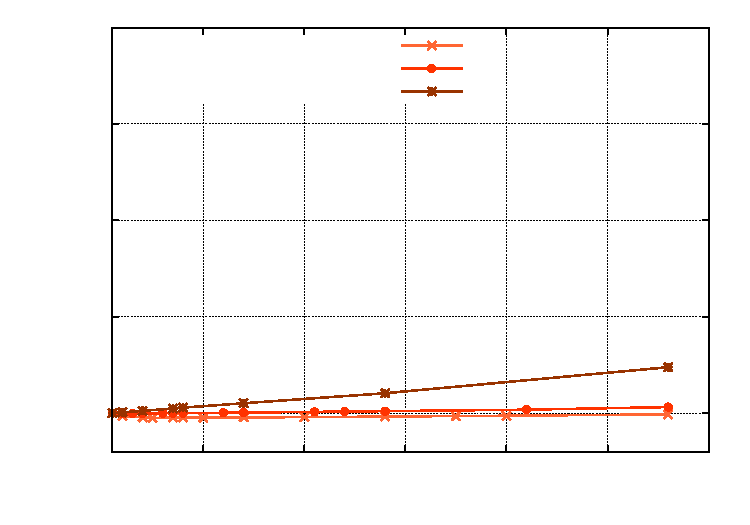
\includegraphics{plot-rowCalcT_nogatherFloat_00_500_4000_all}}%
    \gplfronttext
  \end{picture}%
\endgroup
}
    \caption{Tempi di calcolo di una singola Row $\cdot$ Col con Ta=4000, canali UDN e dati Float}
  \end{subfigure}
  ~
  \begin{subfigure}[b]{.5\textwidth}
    \centering
    \resizebox{\columnwidth}{!}{% GNUPLOT: LaTeX picture with Postscript
\begingroup
  \makeatletter
  \providecommand\color[2][]{%
    \GenericError{(gnuplot) \space\space\space\@spaces}{%
      Package color not loaded in conjunction with
      terminal option `colourtext'%
    }{See the gnuplot documentation for explanation.%
    }{Either use 'blacktext' in gnuplot or load the package
      color.sty in LaTeX.}%
    \renewcommand\color[2][]{}%
  }%
  \providecommand\includegraphics[2][]{%
    \GenericError{(gnuplot) \space\space\space\@spaces}{%
      Package graphicx or graphics not loaded%
    }{See the gnuplot documentation for explanation.%
    }{The gnuplot epslatex terminal needs graphicx.sty or graphics.sty.}%
    \renewcommand\includegraphics[2][]{}%
  }%
  \providecommand\rotatebox[2]{#2}%
  \@ifundefined{ifGPcolor}{%
    \newif\ifGPcolor
    \GPcolortrue
  }{}%
  \@ifundefined{ifGPblacktext}{%
    \newif\ifGPblacktext
    \GPblacktextfalse
  }{}%
  % define a \g@addto@macro without @ in the name:
  \let\gplgaddtomacro\g@addto@macro
  % define empty templates for all commands taking text:
  \gdef\gplbacktext{}%
  \gdef\gplfronttext{}%
  \makeatother
  \ifGPblacktext
    % no textcolor at all
    \def\colorrgb#1{}%
    \def\colorgray#1{}%
  \else
    % gray or color?
    \ifGPcolor
      \def\colorrgb#1{\color[rgb]{#1}}%
      \def\colorgray#1{\color[gray]{#1}}%
      \expandafter\def\csname LTw\endcsname{\color{white}}%
      \expandafter\def\csname LTb\endcsname{\color{black}}%
      \expandafter\def\csname LTa\endcsname{\color{black}}%
      \expandafter\def\csname LT0\endcsname{\color[rgb]{1,0,0}}%
      \expandafter\def\csname LT1\endcsname{\color[rgb]{0,1,0}}%
      \expandafter\def\csname LT2\endcsname{\color[rgb]{0,0,1}}%
      \expandafter\def\csname LT3\endcsname{\color[rgb]{1,0,1}}%
      \expandafter\def\csname LT4\endcsname{\color[rgb]{0,1,1}}%
      \expandafter\def\csname LT5\endcsname{\color[rgb]{1,1,0}}%
      \expandafter\def\csname LT6\endcsname{\color[rgb]{0,0,0}}%
      \expandafter\def\csname LT7\endcsname{\color[rgb]{1,0.3,0}}%
      \expandafter\def\csname LT8\endcsname{\color[rgb]{0.5,0.5,0.5}}%
    \else
      % gray
      \def\colorrgb#1{\color{black}}%
      \def\colorgray#1{\color[gray]{#1}}%
      \expandafter\def\csname LTw\endcsname{\color{white}}%
      \expandafter\def\csname LTb\endcsname{\color{black}}%
      \expandafter\def\csname LTa\endcsname{\color{black}}%
      \expandafter\def\csname LT0\endcsname{\color{black}}%
      \expandafter\def\csname LT1\endcsname{\color{black}}%
      \expandafter\def\csname LT2\endcsname{\color{black}}%
      \expandafter\def\csname LT3\endcsname{\color{black}}%
      \expandafter\def\csname LT4\endcsname{\color{black}}%
      \expandafter\def\csname LT5\endcsname{\color{black}}%
      \expandafter\def\csname LT6\endcsname{\color{black}}%
      \expandafter\def\csname LT7\endcsname{\color{black}}%
      \expandafter\def\csname LT8\endcsname{\color{black}}%
    \fi
  \fi
  \setlength{\unitlength}{0.0500bp}%
  \begin{picture}(7200.00,5040.00)%
    \gplgaddtomacro\gplbacktext{%
      \csname LTb\endcsname%
      \put(946,1074){\makebox(0,0)[r]{\strut{} 1}}%
      \csname LTb\endcsname%
      \put(946,1999){\makebox(0,0)[r]{\strut{} 1.5}}%
      \csname LTb\endcsname%
      \put(946,2925){\makebox(0,0)[r]{\strut{} 2}}%
      \csname LTb\endcsname%
      \put(946,3850){\makebox(0,0)[r]{\strut{} 2.5}}%
      \csname LTb\endcsname%
      \put(946,4775){\makebox(0,0)[r]{\strut{} 3}}%
      \csname LTb\endcsname%
      \put(1951,484){\makebox(0,0){\strut{} 10}}%
      \csname LTb\endcsname%
      \put(2922,484){\makebox(0,0){\strut{} 20}}%
      \csname LTb\endcsname%
      \put(3892,484){\makebox(0,0){\strut{} 30}}%
      \csname LTb\endcsname%
      \put(4862,484){\makebox(0,0){\strut{} 40}}%
      \csname LTb\endcsname%
      \put(5833,484){\makebox(0,0){\strut{} 50}}%
      \csname LTb\endcsname%
      \put(6803,484){\makebox(0,0){\strut{} 60}}%
      \put(176,2739){\rotatebox{-270}{\makebox(0,0){\strut{}$T_{\textrm{row}}^{\phantom{row}(n)} / T_{\textrm{row}}^{\phantom{row}(1)}$}}}%
      \put(3940,154){\makebox(0,0){\strut{}$n$ parallel degree}}%
    }%
    \gplgaddtomacro\gplfronttext{%
      \csname LTb\endcsname%
      \put(3718,4602){\makebox(0,0)[r]{\strut{}Matrix Size 280x280}}%
      \csname LTb\endcsname%
      \put(3718,4382){\makebox(0,0)[r]{\strut{}Matrix Size 168x168}}%
      \csname LTb\endcsname%
      \put(3718,4162){\makebox(0,0)[r]{\strut{}Matrix Size 56x56}}%
    }%
    \gplbacktext
    \put(0,0){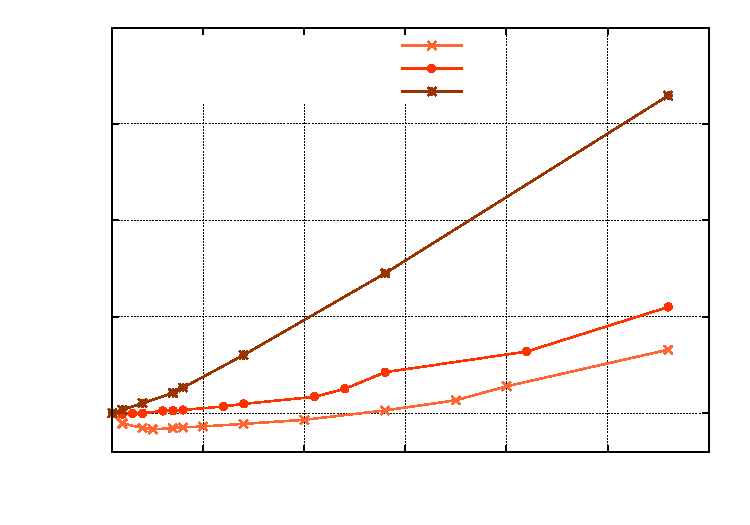
\includegraphics{plot-rowCalcT_nogatherInt_11_500_4000_all}}%
    \gplfronttext
  \end{picture}%
\endgroup
}
    \caption{Tempi di calcolo di una singola Row $\cdot$ Col con Ta=4000, canali SM e dati Int}
  \end{subfigure}
  \hspace{2ex}
  \begin{subfigure}[b]{.5\textwidth}
    \centering
    \resizebox{\columnwidth}{!}{% GNUPLOT: LaTeX picture with Postscript
\begingroup
  \makeatletter
  \providecommand\color[2][]{%
    \GenericError{(gnuplot) \space\space\space\@spaces}{%
      Package color not loaded in conjunction with
      terminal option `colourtext'%
    }{See the gnuplot documentation for explanation.%
    }{Either use 'blacktext' in gnuplot or load the package
      color.sty in LaTeX.}%
    \renewcommand\color[2][]{}%
  }%
  \providecommand\includegraphics[2][]{%
    \GenericError{(gnuplot) \space\space\space\@spaces}{%
      Package graphicx or graphics not loaded%
    }{See the gnuplot documentation for explanation.%
    }{The gnuplot epslatex terminal needs graphicx.sty or graphics.sty.}%
    \renewcommand\includegraphics[2][]{}%
  }%
  \providecommand\rotatebox[2]{#2}%
  \@ifundefined{ifGPcolor}{%
    \newif\ifGPcolor
    \GPcolortrue
  }{}%
  \@ifundefined{ifGPblacktext}{%
    \newif\ifGPblacktext
    \GPblacktextfalse
  }{}%
  % define a \g@addto@macro without @ in the name:
  \let\gplgaddtomacro\g@addto@macro
  % define empty templates for all commands taking text:
  \gdef\gplbacktext{}%
  \gdef\gplfronttext{}%
  \makeatother
  \ifGPblacktext
    % no textcolor at all
    \def\colorrgb#1{}%
    \def\colorgray#1{}%
  \else
    % gray or color?
    \ifGPcolor
      \def\colorrgb#1{\color[rgb]{#1}}%
      \def\colorgray#1{\color[gray]{#1}}%
      \expandafter\def\csname LTw\endcsname{\color{white}}%
      \expandafter\def\csname LTb\endcsname{\color{black}}%
      \expandafter\def\csname LTa\endcsname{\color{black}}%
      \expandafter\def\csname LT0\endcsname{\color[rgb]{1,0,0}}%
      \expandafter\def\csname LT1\endcsname{\color[rgb]{0,1,0}}%
      \expandafter\def\csname LT2\endcsname{\color[rgb]{0,0,1}}%
      \expandafter\def\csname LT3\endcsname{\color[rgb]{1,0,1}}%
      \expandafter\def\csname LT4\endcsname{\color[rgb]{0,1,1}}%
      \expandafter\def\csname LT5\endcsname{\color[rgb]{1,1,0}}%
      \expandafter\def\csname LT6\endcsname{\color[rgb]{0,0,0}}%
      \expandafter\def\csname LT7\endcsname{\color[rgb]{1,0.3,0}}%
      \expandafter\def\csname LT8\endcsname{\color[rgb]{0.5,0.5,0.5}}%
    \else
      % gray
      \def\colorrgb#1{\color{black}}%
      \def\colorgray#1{\color[gray]{#1}}%
      \expandafter\def\csname LTw\endcsname{\color{white}}%
      \expandafter\def\csname LTb\endcsname{\color{black}}%
      \expandafter\def\csname LTa\endcsname{\color{black}}%
      \expandafter\def\csname LT0\endcsname{\color{black}}%
      \expandafter\def\csname LT1\endcsname{\color{black}}%
      \expandafter\def\csname LT2\endcsname{\color{black}}%
      \expandafter\def\csname LT3\endcsname{\color{black}}%
      \expandafter\def\csname LT4\endcsname{\color{black}}%
      \expandafter\def\csname LT5\endcsname{\color{black}}%
      \expandafter\def\csname LT6\endcsname{\color{black}}%
      \expandafter\def\csname LT7\endcsname{\color{black}}%
      \expandafter\def\csname LT8\endcsname{\color{black}}%
    \fi
  \fi
  \setlength{\unitlength}{0.0500bp}%
  \begin{picture}(7200.00,5040.00)%
    \gplgaddtomacro\gplbacktext{%
      \csname LTb\endcsname%
      \put(946,1074){\makebox(0,0)[r]{\strut{} 1}}%
      \csname LTb\endcsname%
      \put(946,1999){\makebox(0,0)[r]{\strut{} 1.5}}%
      \csname LTb\endcsname%
      \put(946,2925){\makebox(0,0)[r]{\strut{} 2}}%
      \csname LTb\endcsname%
      \put(946,3850){\makebox(0,0)[r]{\strut{} 2.5}}%
      \csname LTb\endcsname%
      \put(946,4775){\makebox(0,0)[r]{\strut{} 3}}%
      \csname LTb\endcsname%
      \put(1951,484){\makebox(0,0){\strut{} 10}}%
      \csname LTb\endcsname%
      \put(2922,484){\makebox(0,0){\strut{} 20}}%
      \csname LTb\endcsname%
      \put(3892,484){\makebox(0,0){\strut{} 30}}%
      \csname LTb\endcsname%
      \put(4862,484){\makebox(0,0){\strut{} 40}}%
      \csname LTb\endcsname%
      \put(5833,484){\makebox(0,0){\strut{} 50}}%
      \csname LTb\endcsname%
      \put(6803,484){\makebox(0,0){\strut{} 60}}%
      \put(176,2739){\rotatebox{-270}{\makebox(0,0){\strut{}$T_{\textrm{row}}^{\phantom{row}(n)} / T_{\textrm{row}}^{\phantom{row}(1)}$}}}%
      \put(3940,154){\makebox(0,0){\strut{}$n$ parallel degree}}%
    }%
    \gplgaddtomacro\gplfronttext{%
      \csname LTb\endcsname%
      \put(3718,4602){\makebox(0,0)[r]{\strut{}Matrix Size 280x280}}%
      \csname LTb\endcsname%
      \put(3718,4382){\makebox(0,0)[r]{\strut{}Matrix Size 168x168}}%
      \csname LTb\endcsname%
      \put(3718,4162){\makebox(0,0)[r]{\strut{}Matrix Size 56x56}}%
    }%
    \gplbacktext
    \put(0,0){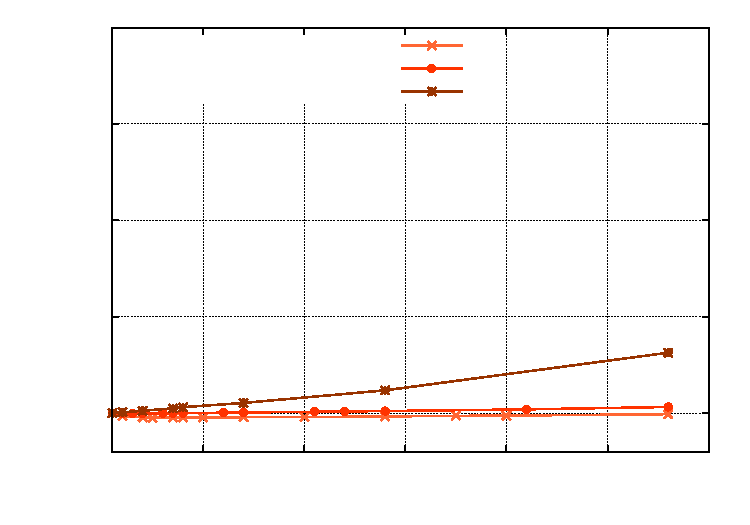
\includegraphics{plot-rowCalcT_nogatherFloat_11_500_4000_all}}%
    \gplfronttext
  \end{picture}%
\endgroup
}
    \caption{Tempi di calcolo di una singola Row $\cdot$ Col con Ta=4000, canali SM e dati Float}
  \end{subfigure}
\end{figure}

\FloatBarrier



%%%%%%%%%%%%%%%%%%%%%%%%%%%%%%%%%%%%%%%%%%%%%%%%%%%%%%%%%%%%%%%%%%%%%%%%%%%%%%%%

%% \newpage
%% \FloatBarrier
\subsection{Data}

\lstinputlisting[firstline=4, style=data, caption={complete time: UDN, M=56, \Ta=4000}, float=h  ]{nogatherInt_00_500_4000_56.dat.avg}
\lstinputlisting[firstline=4, style=data, caption={service time: UDN, M=56, \Ta=4000}, float=h  ]{nogatherInt_00_500_4000_56_servicetime.dat.avg}

\lstinputlisting[firstline=4, style=data, caption={complete time: UDN, M=280, \Ta=50000}, float=h  ]{nogatherInt_00_500_50000_280.dat.avg}
\lstinputlisting[firstline=4, style=data, caption={service time: UDN, M=280, \Ta=50000}, float=h  ]{nogatherInt_00_500_50000_280_servicetime.dat.avg}

\lstinputlisting[firstline=4, style=data, caption={complete time: SM, M=56, \Ta=4000}, float=h  ]{nogatherInt_11_500_4000_56.dat.avg}
\lstinputlisting[firstline=4, style=data, caption={service time: SM, M=56, \Ta=4000}, float=h  ]{nogatherInt_11_500_4000_56_servicetime.dat.avg}

\lstinputlisting[firstline=4, style=data, caption={complete time: SM, M=280, \Ta=50000}, float=h  ]{nogatherInt_11_500_50000_280.dat.avg}
\lstinputlisting[firstline=4, style=data, caption={service time: SM, M=280, \Ta=50000}, float=h  ]{nogatherInt_11_500_50000_280_servicetime.dat.avg}


\lstinputlisting[firstline=4, style=data, caption={multicast service time: UDN, M=56, \Ta=50000}, float=h  ]{nogatherInt_00_500_4000_56_multictime.dbg.avg}
\lstinputlisting[firstline=4, style=data, caption={multicast service time: SM, M=56, \Ta=50000}, float=h  ]{nogatherInt_11_500_4000_56_multictime.dbg.avg}

\lstinputlisting[firstline=4, style=data, caption={multicast service time: UDN, M=168, \Ta=50000}, float=h  ]{nogatherInt_00_500_20000_168_multictime.dbg.avg}
\lstinputlisting[firstline=4, style=data, caption={multicast service time: SM, M=168, \Ta=50000}, float=h  ]{nogatherInt_11_500_20000_168_multictime.dbg.avg}

\lstinputlisting[firstline=4, style=data, caption={multicast service time: UDN, M=280, \Ta=50000}, float=h  ]{nogatherInt_00_500_50000_280_multictime.dbg.avg}
\lstinputlisting[firstline=4, style=data, caption={multicast service time: SM, M=280, \Ta=50000}, float=h  ]{nogatherInt_11_500_50000_280_multictime.dbg.avg}



%%%%%%%%%%%%%%%%%%%%%%%%%%%%%%%%%%%%%%%%%%%%%%%%%%%%%%%%%%%%%%%%%%%%%%%%%%%%%%%%


%% \newpage

%% \FloatBarrier
%% \begin{figure}[p]
%%   \centering
%%   \resizebox{\columnwidth}{!}{\input{plot3_nogatherInt_all_500_4000_56.tex}}
%% \end{figure}

\end{document}
